\chapter{Additional Plots}\label{ch:additional_plots}


\section{ORB Comparison Plots}\label{sec:ORBcomp}{

    \begin{figure}[ht]
        \centering
        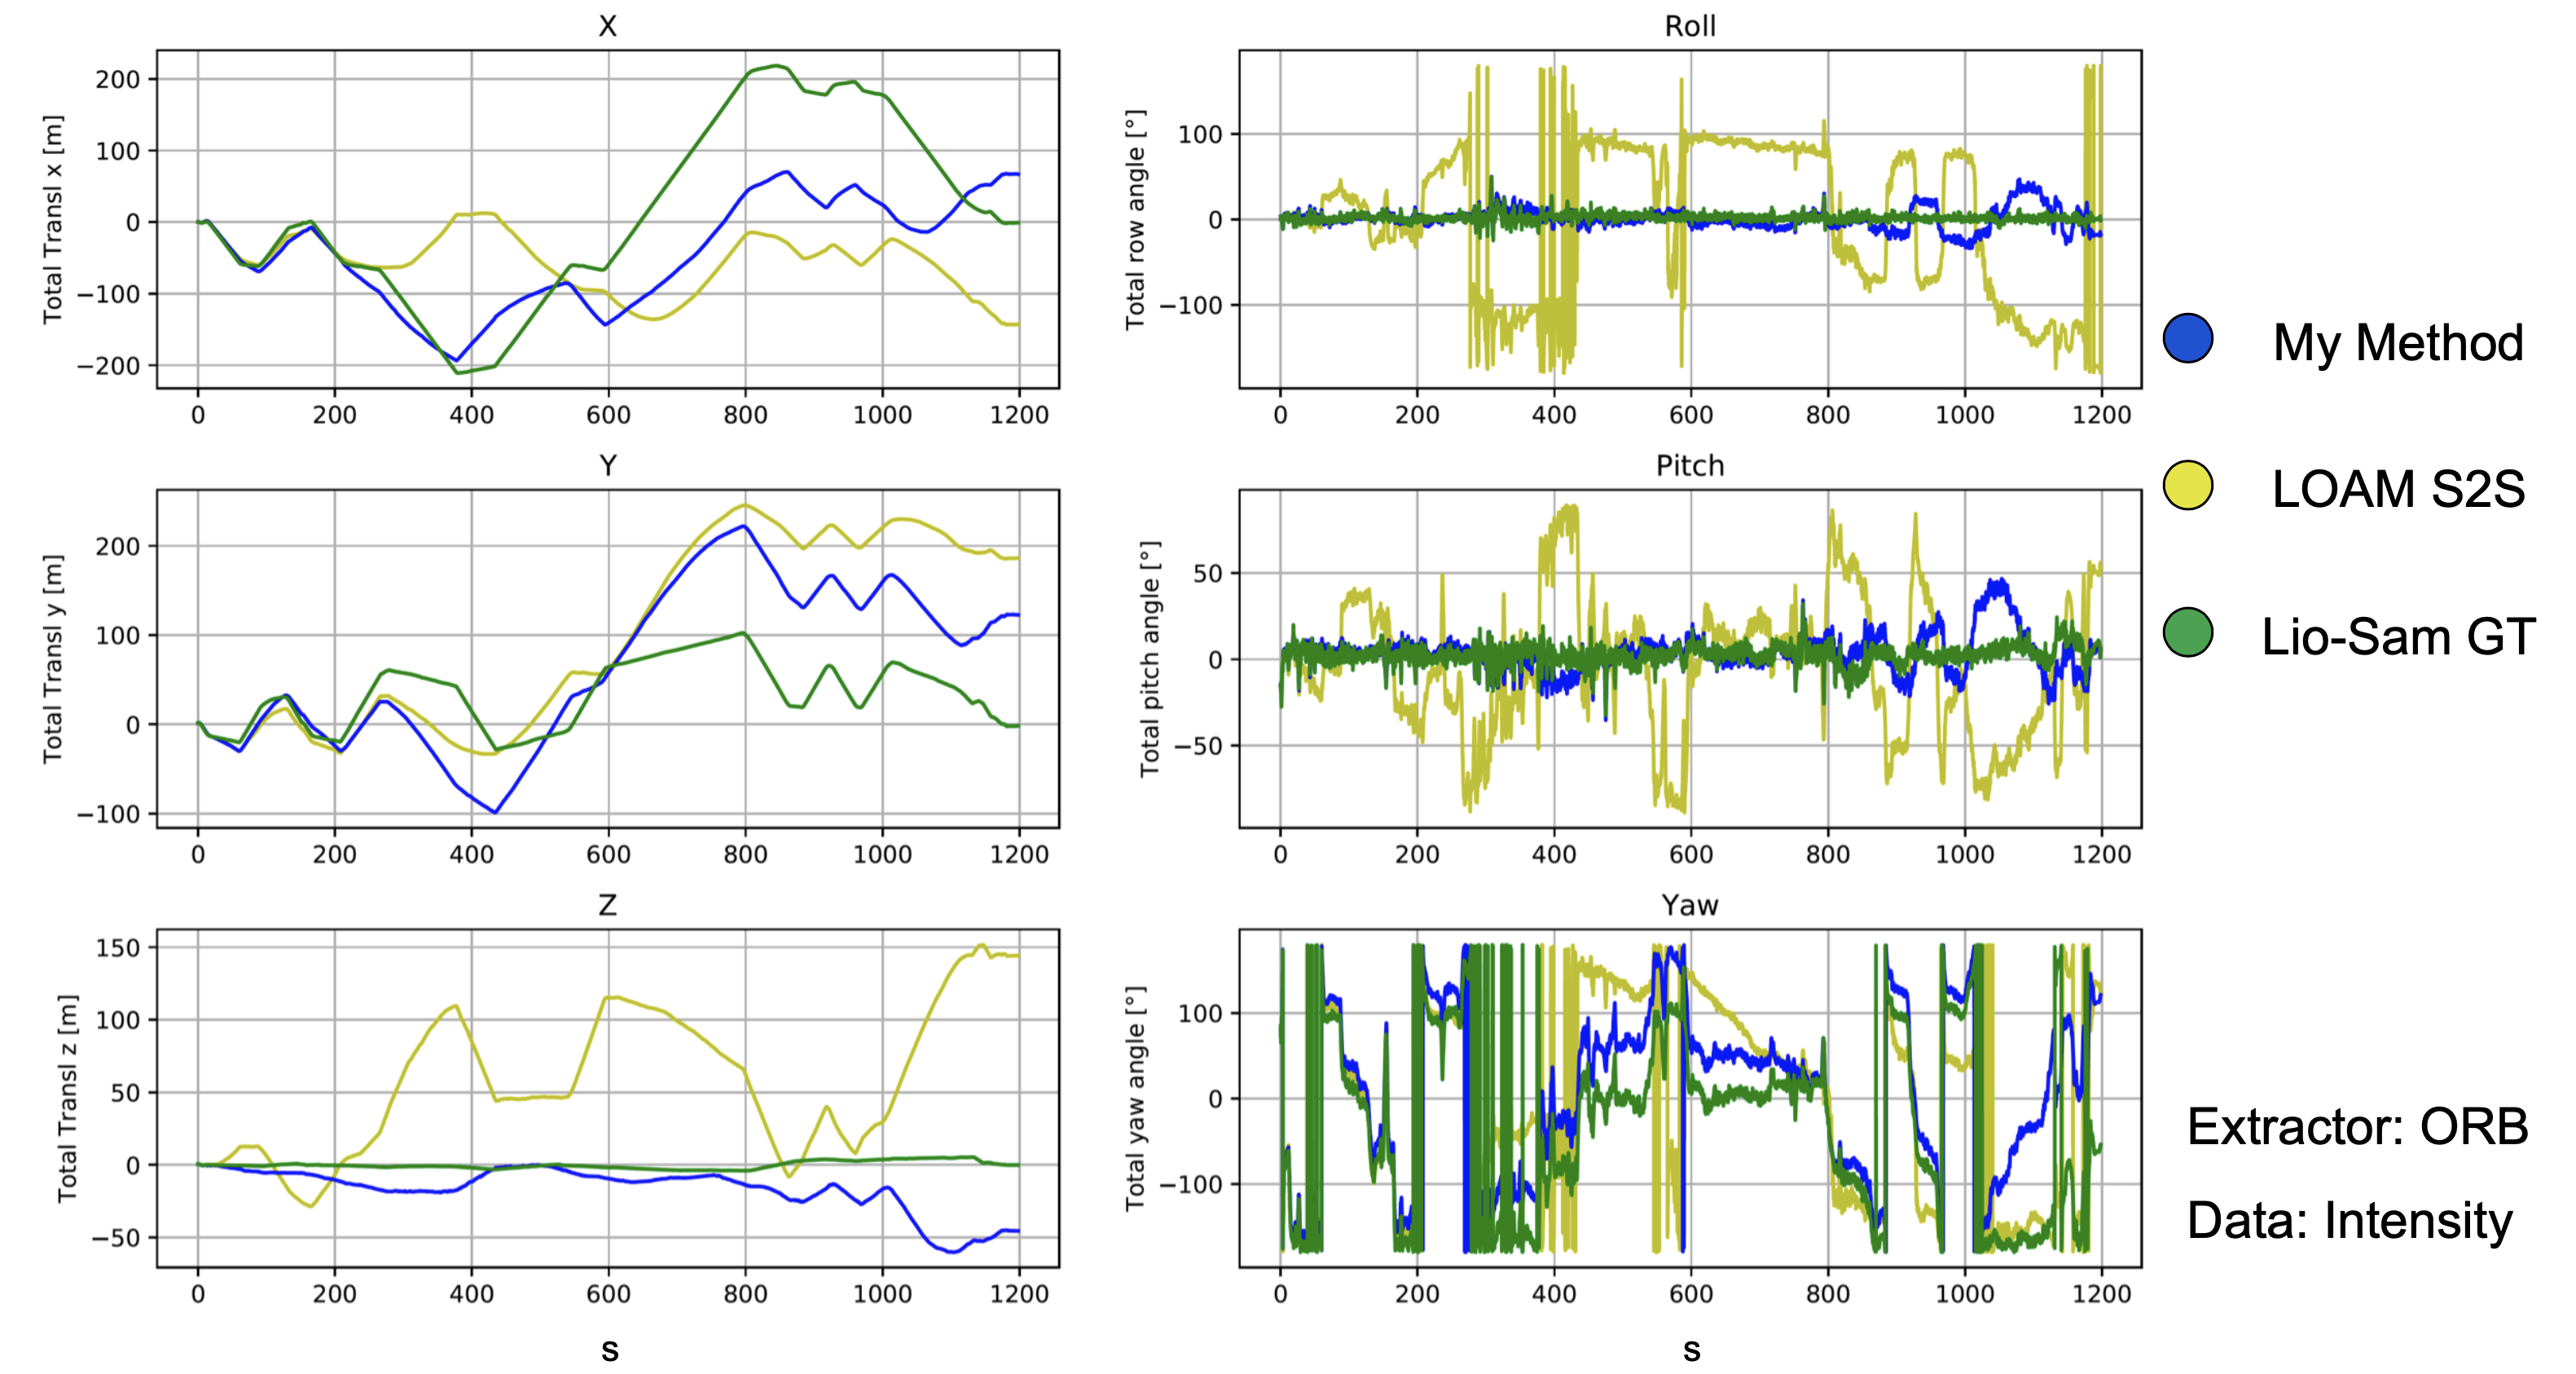
\includegraphics[scale = 0.25]{images/comparison_appendix/pose_orb.png}
        \caption{Pose comparison orb}
        \label{fig:pose_comparison_orb}
    \end{figure}
    \clearpage
    
    \begin{figure}[ht]
        \centering
        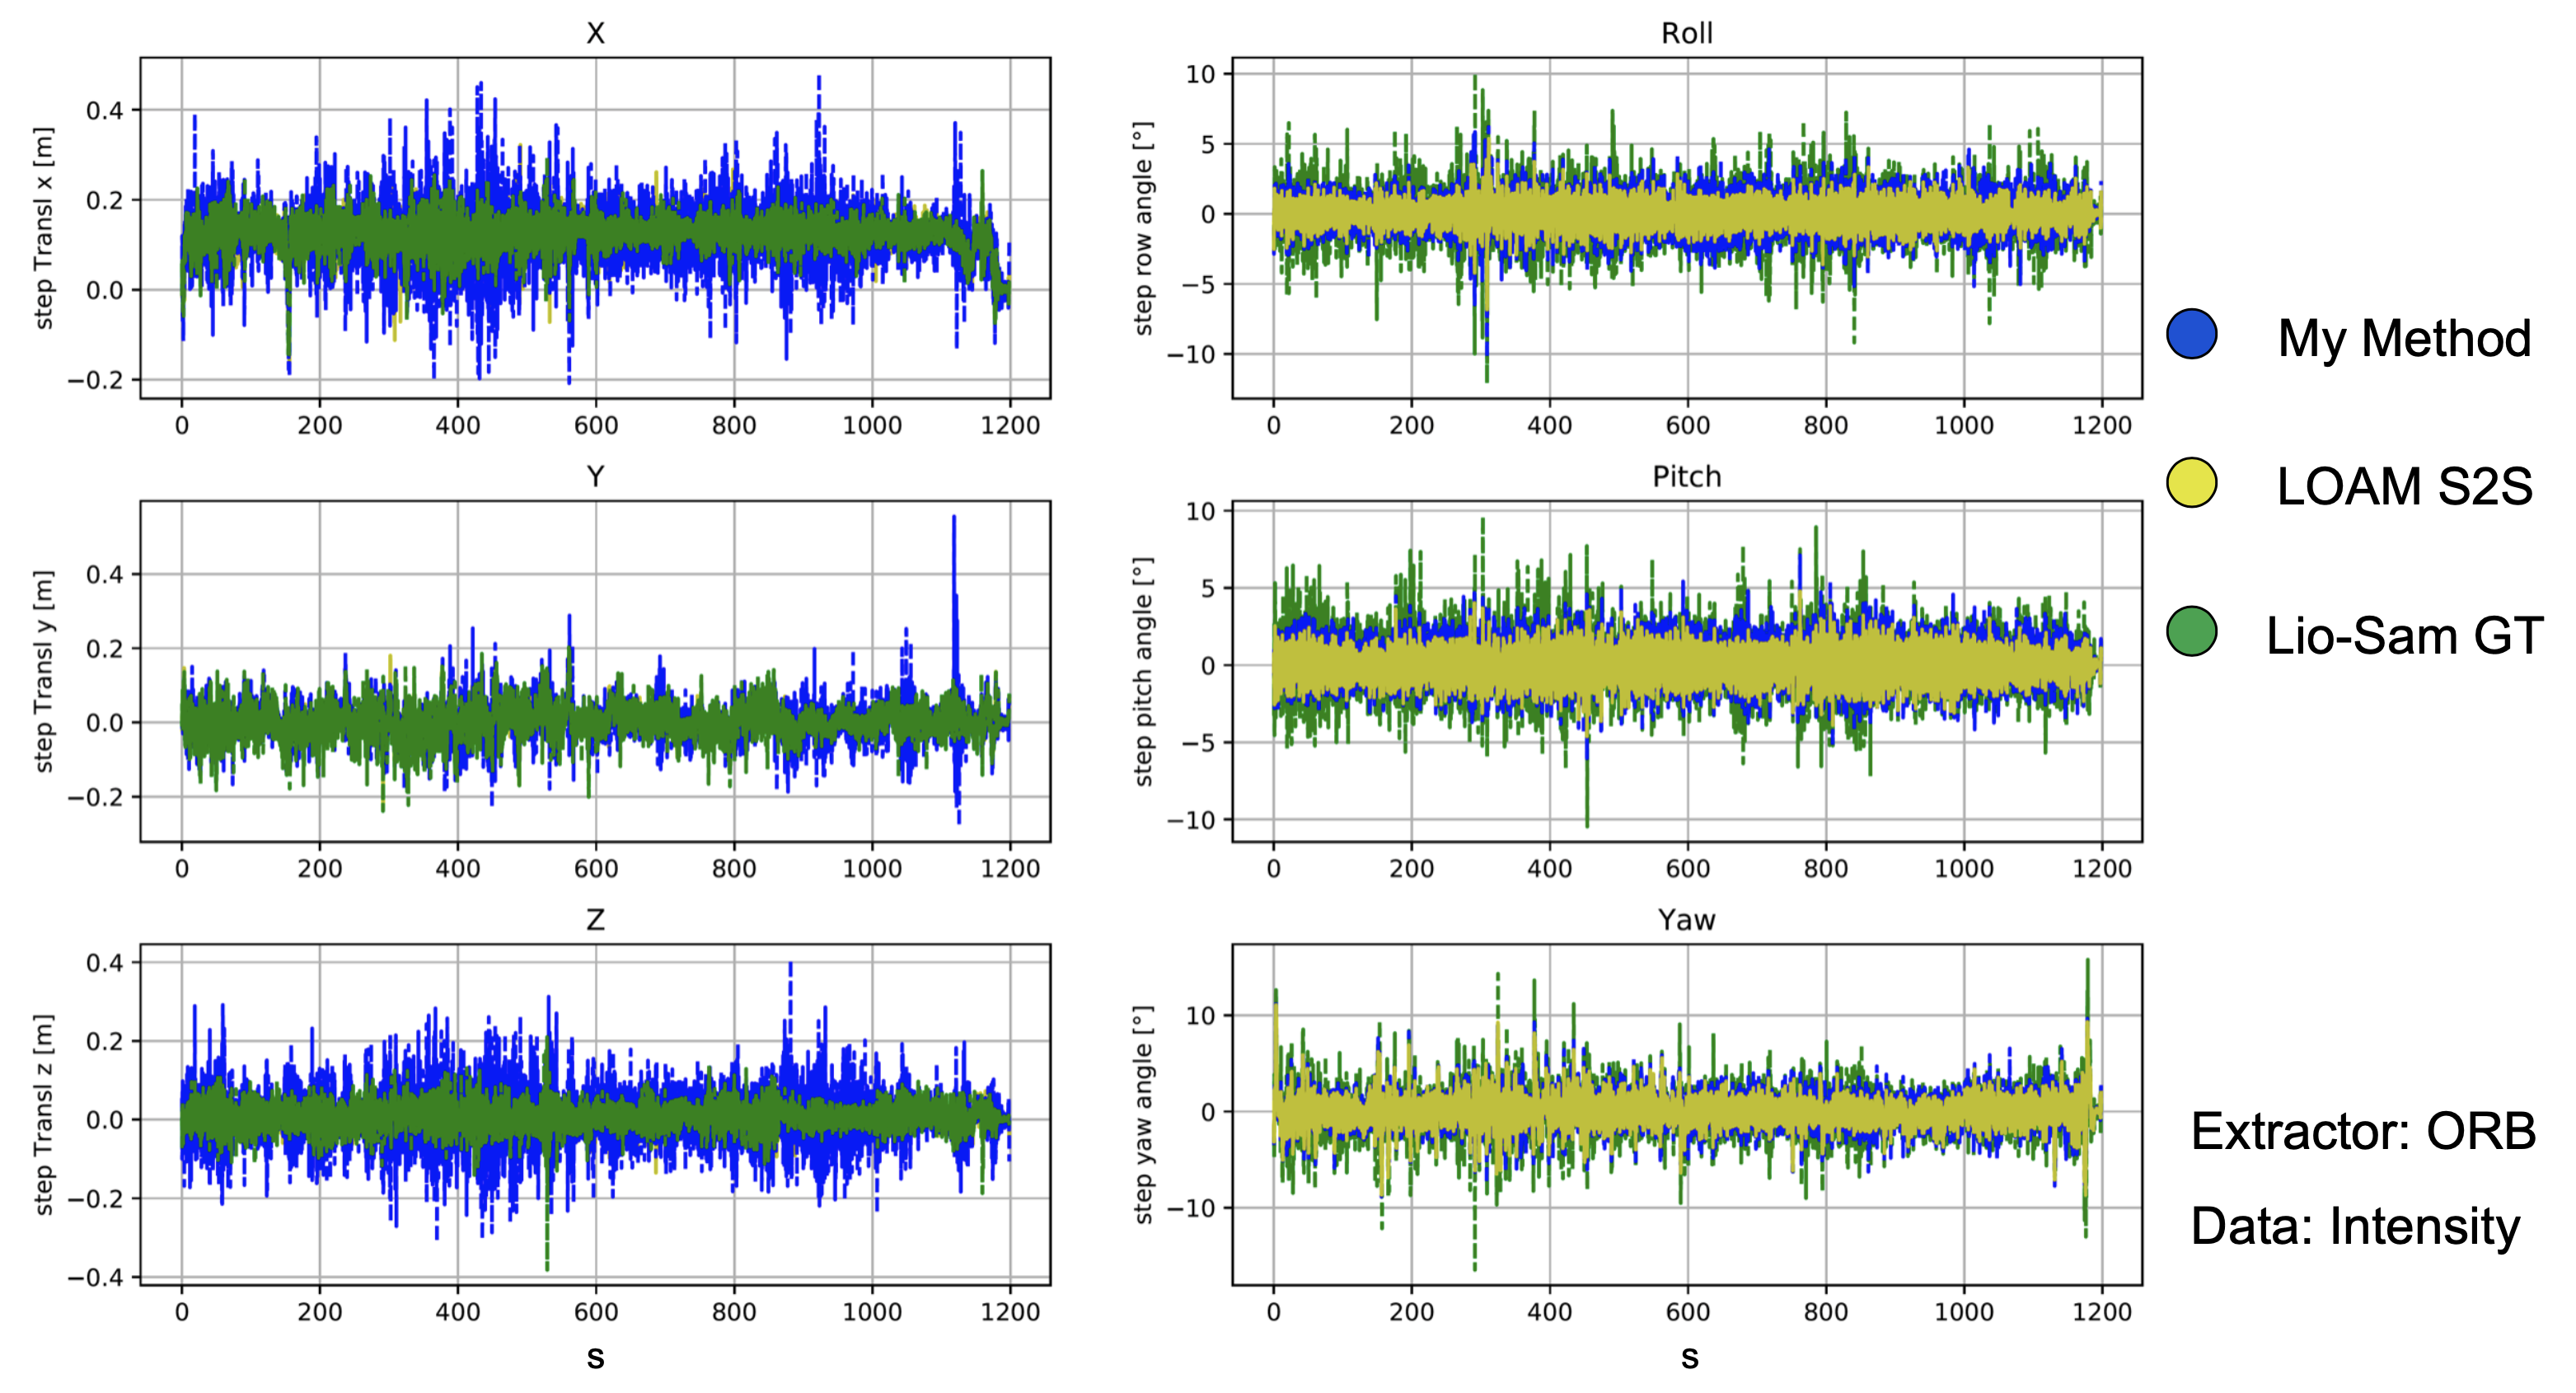
\includegraphics[scale = 0.25]{images/comparison_appendix/steps_orb.png}
        \caption{Step comparison orb}
        \label{fig:step_comparison_orb}
    \end{figure}

    \begin{figure}[ht]
        \centering
        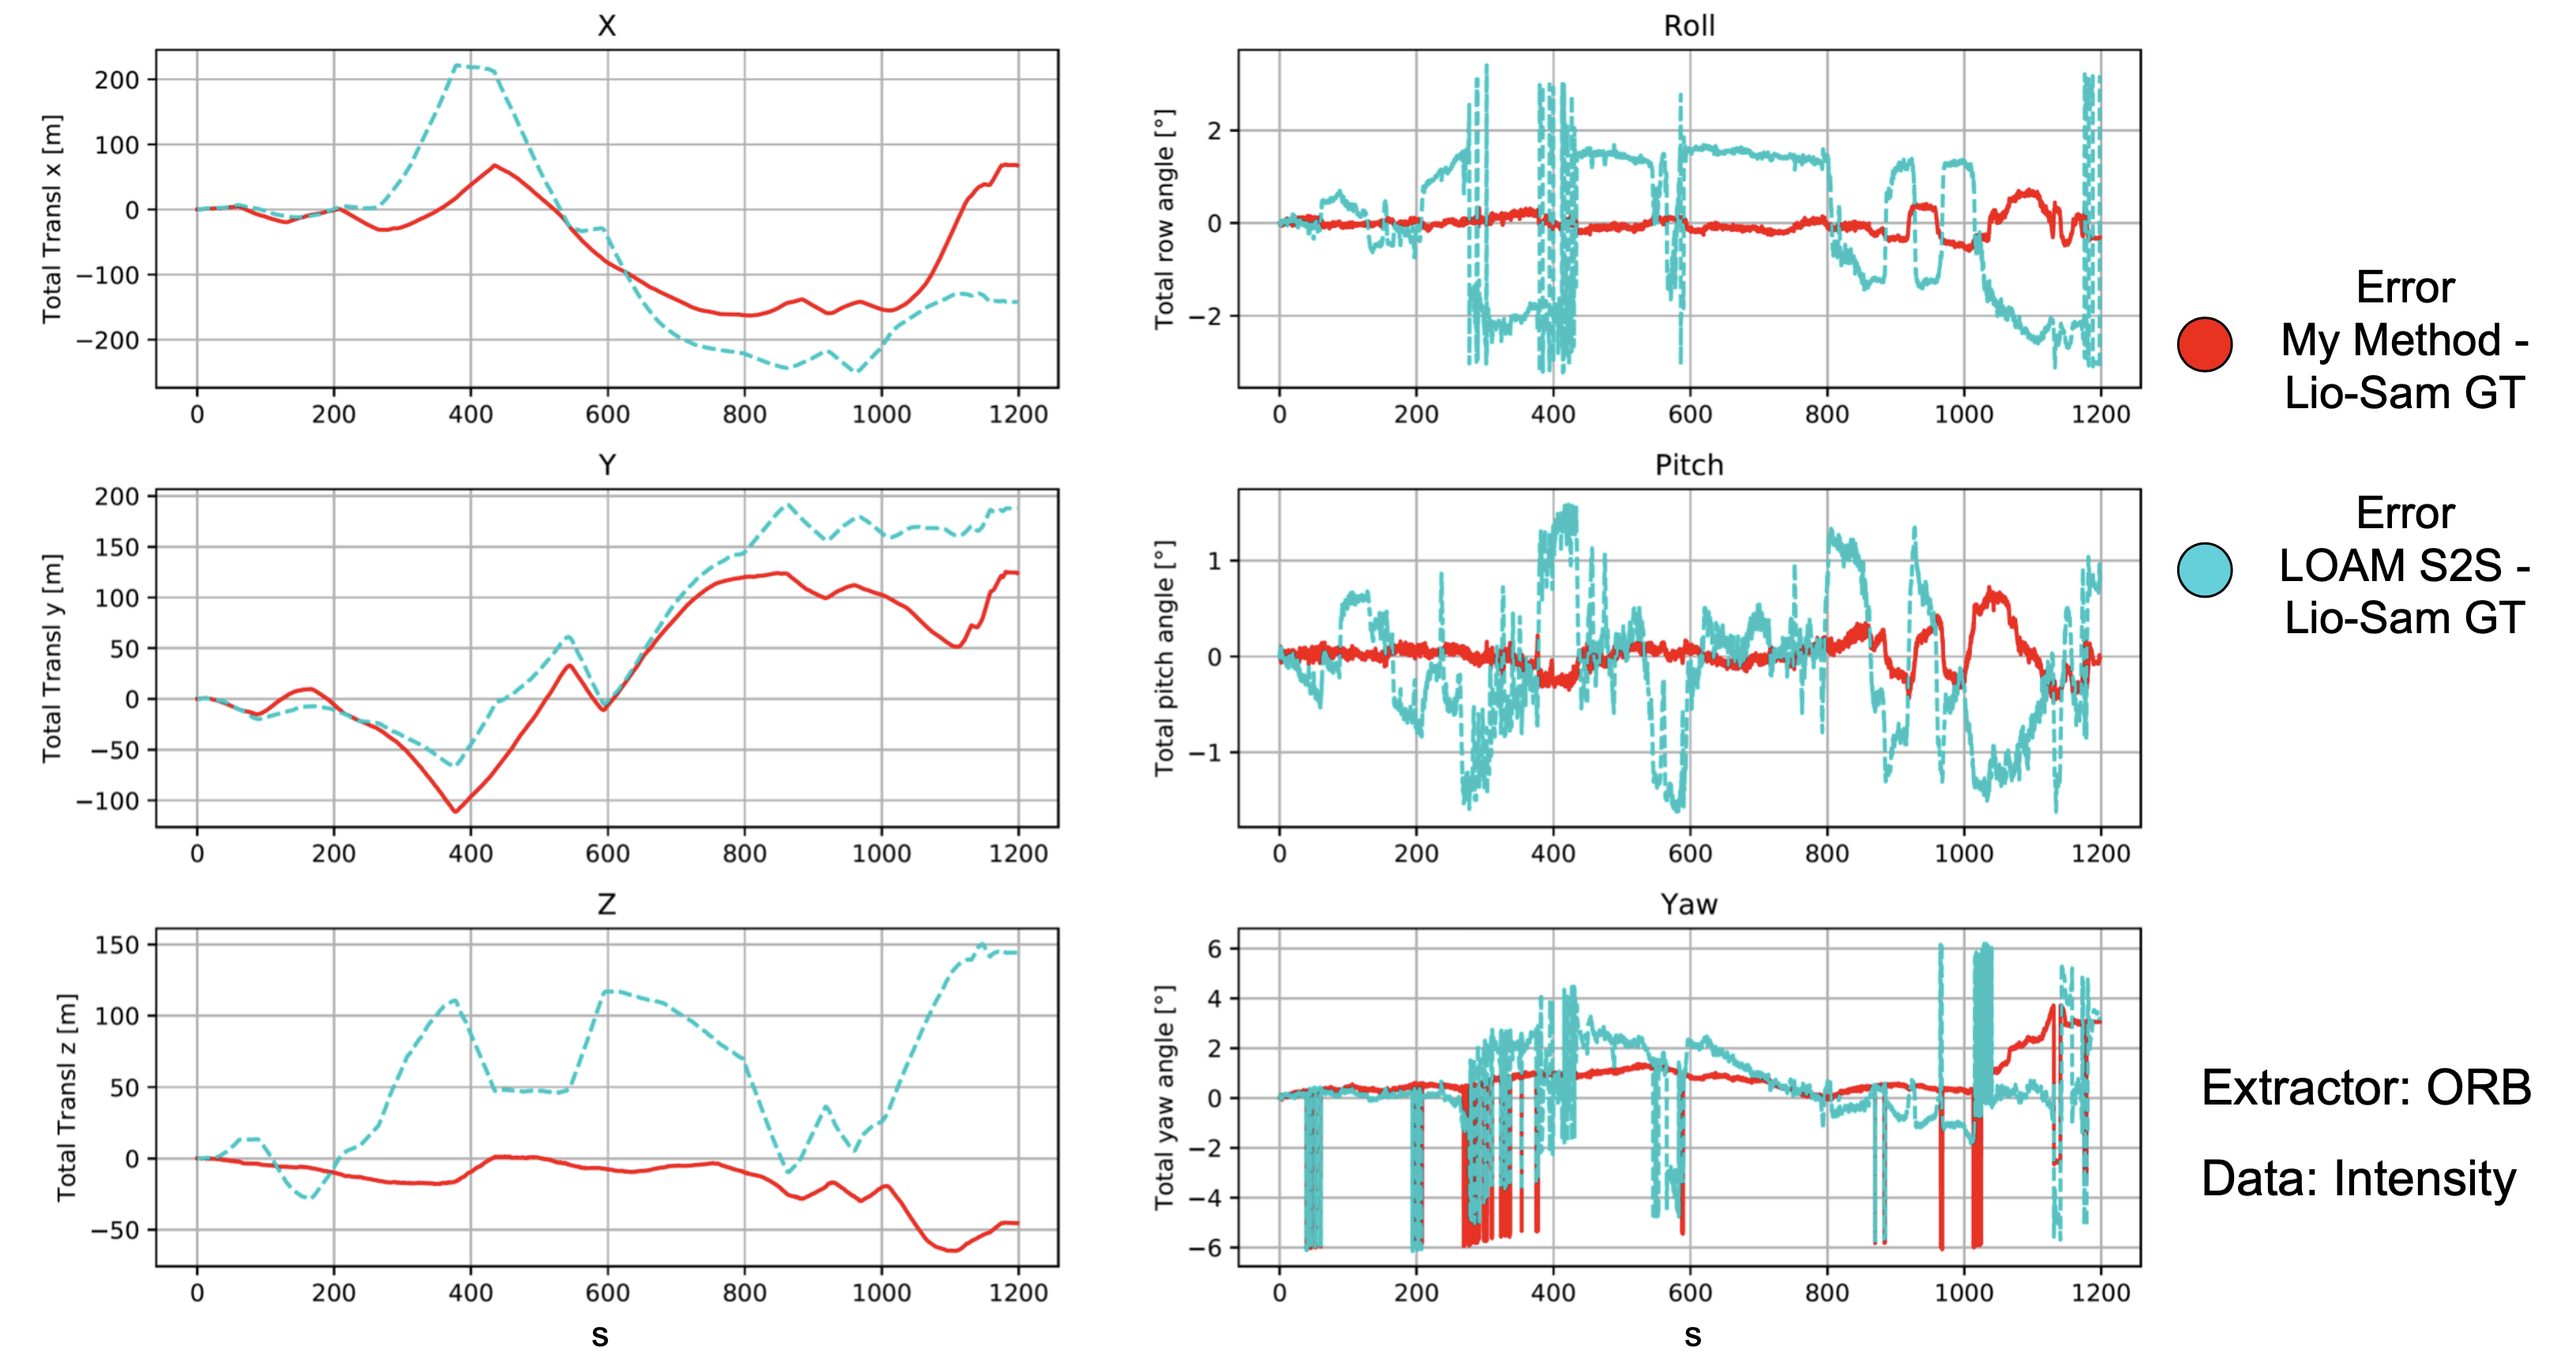
\includegraphics[scale = 0.25]{images/comparison_appendix/pose_error_orb.png}
        \caption{Pose error comparison orb}
        \label{fig:pose_error_comparison_orb}
    \end{figure}
    \clearpage
    
    \begin{figure}[ht]
        \centering
        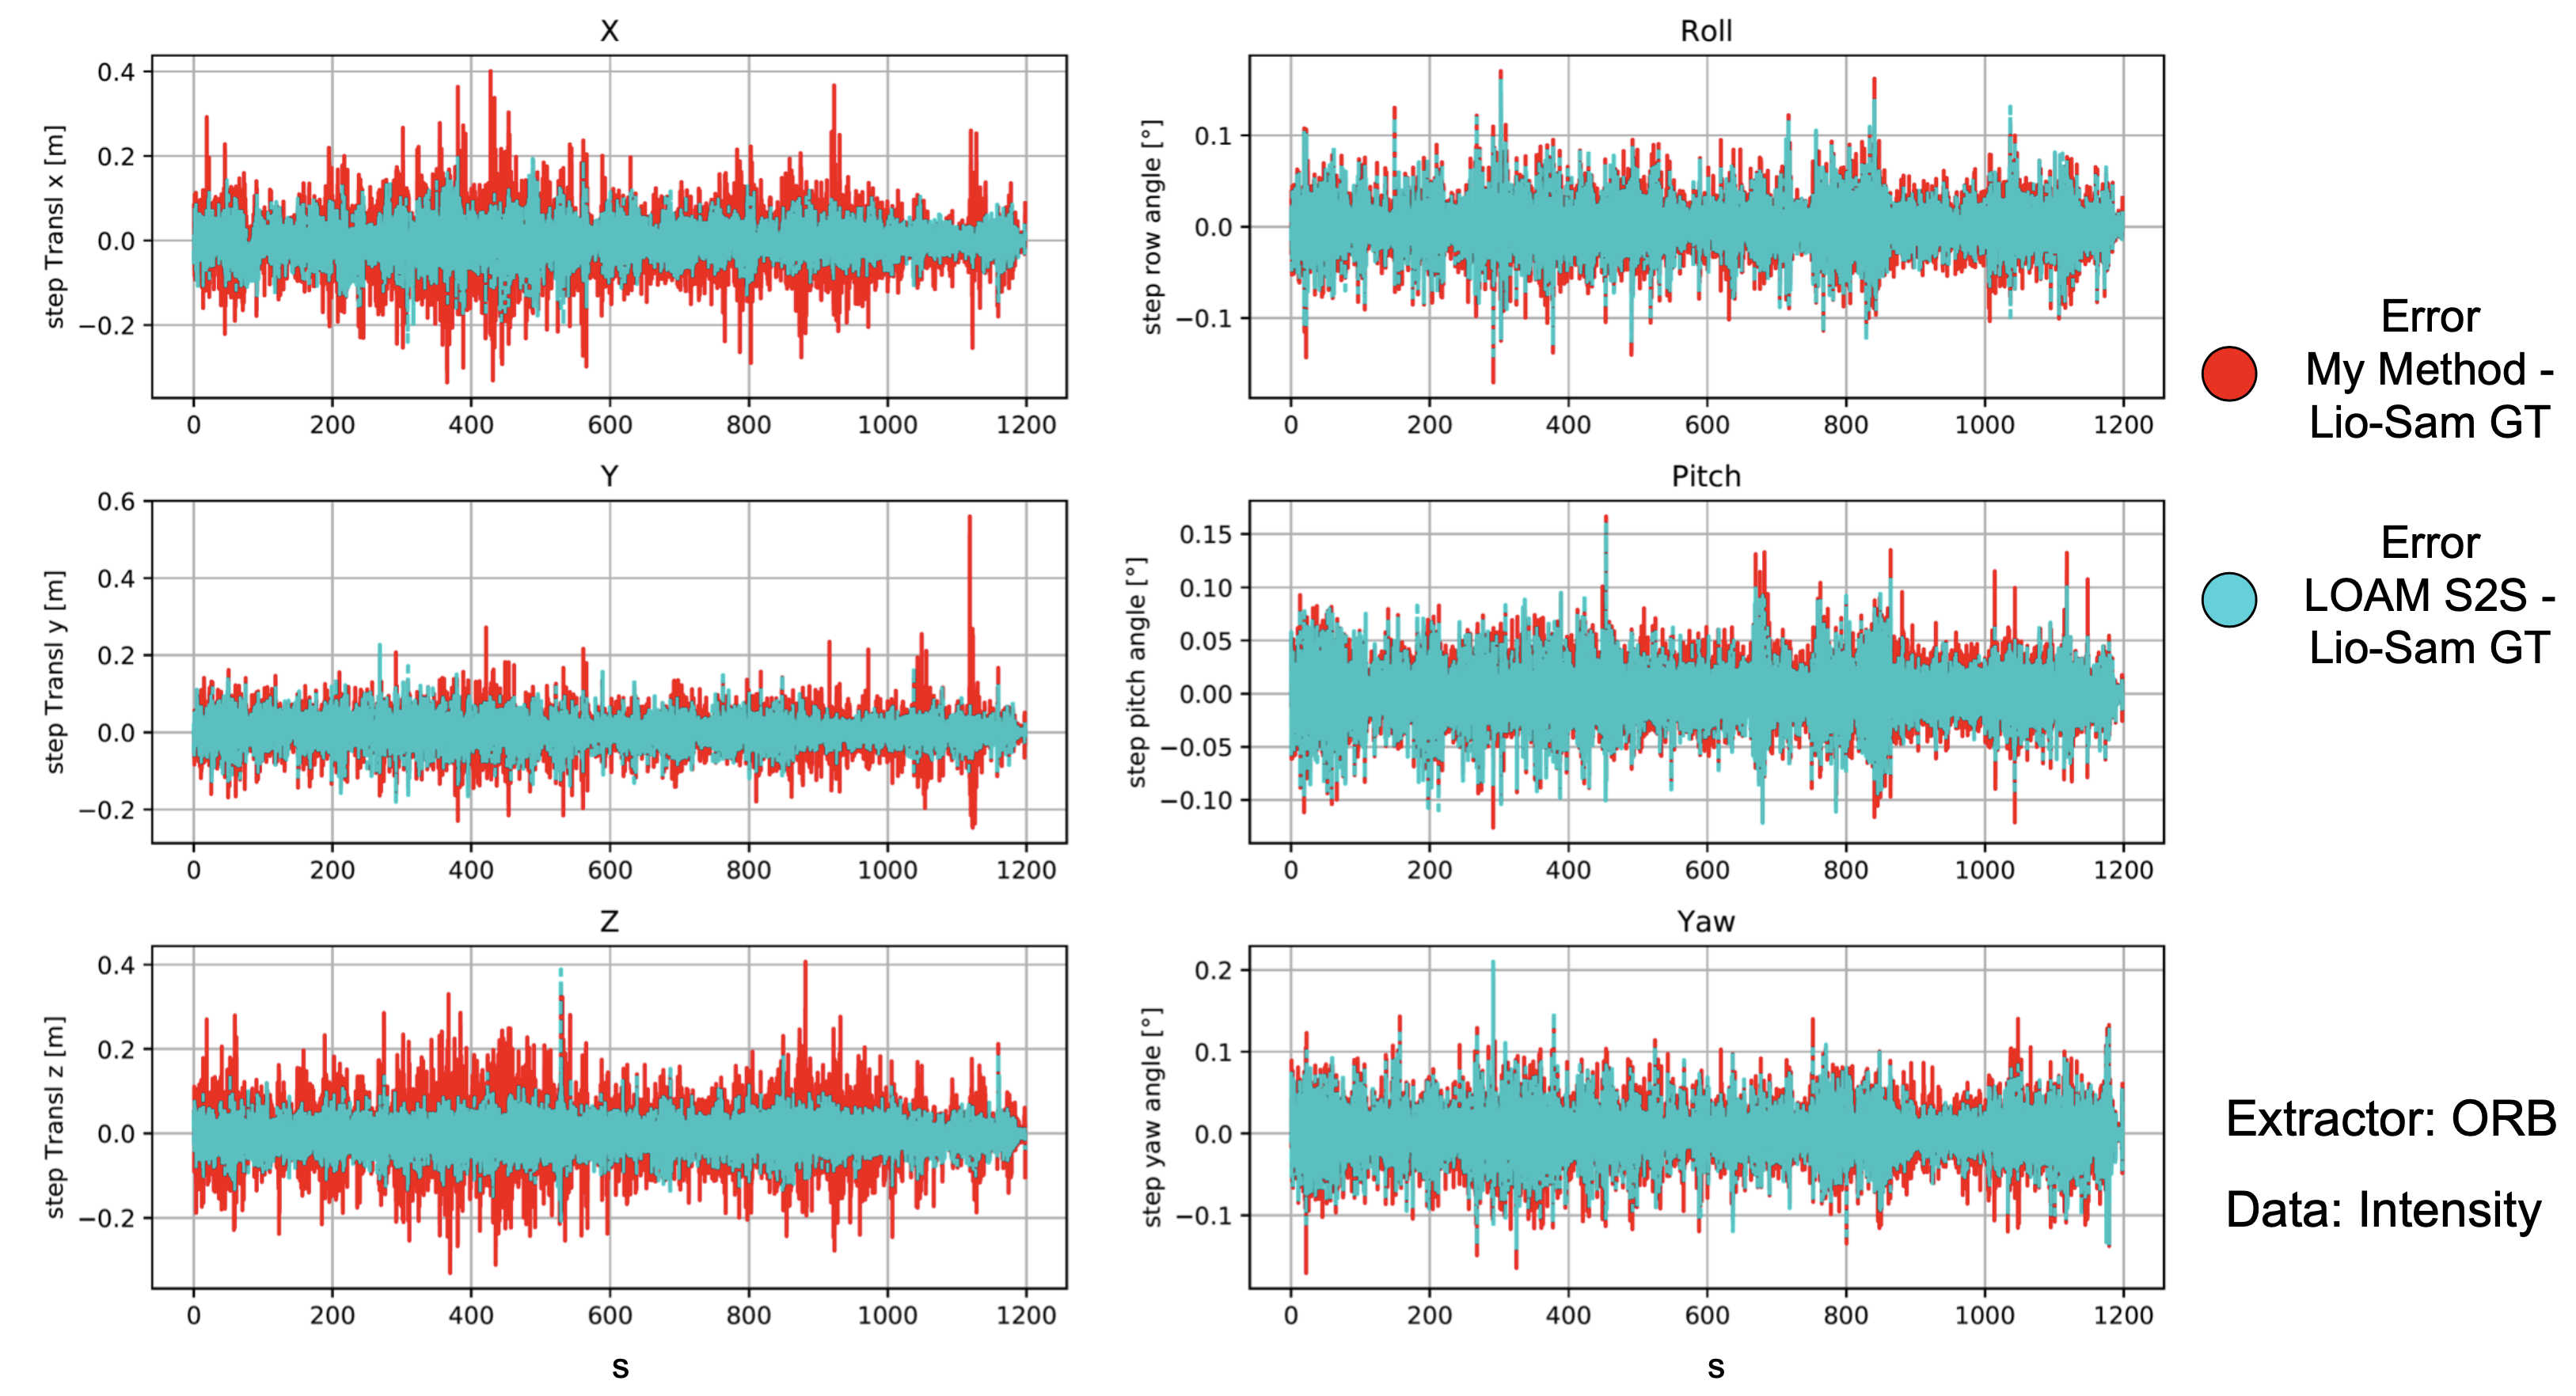
\includegraphics[scale = 0.25]{images/comparison_appendix/step_error_orb.png}
        \caption{Step error comparison orb}
        \label{fig:step_error_comparison_orb}
    \end{figure}
    \clearpage
}
    



\section{BRISK Comparison Plots}{

    \begin{figure}[ht]
        \centering
        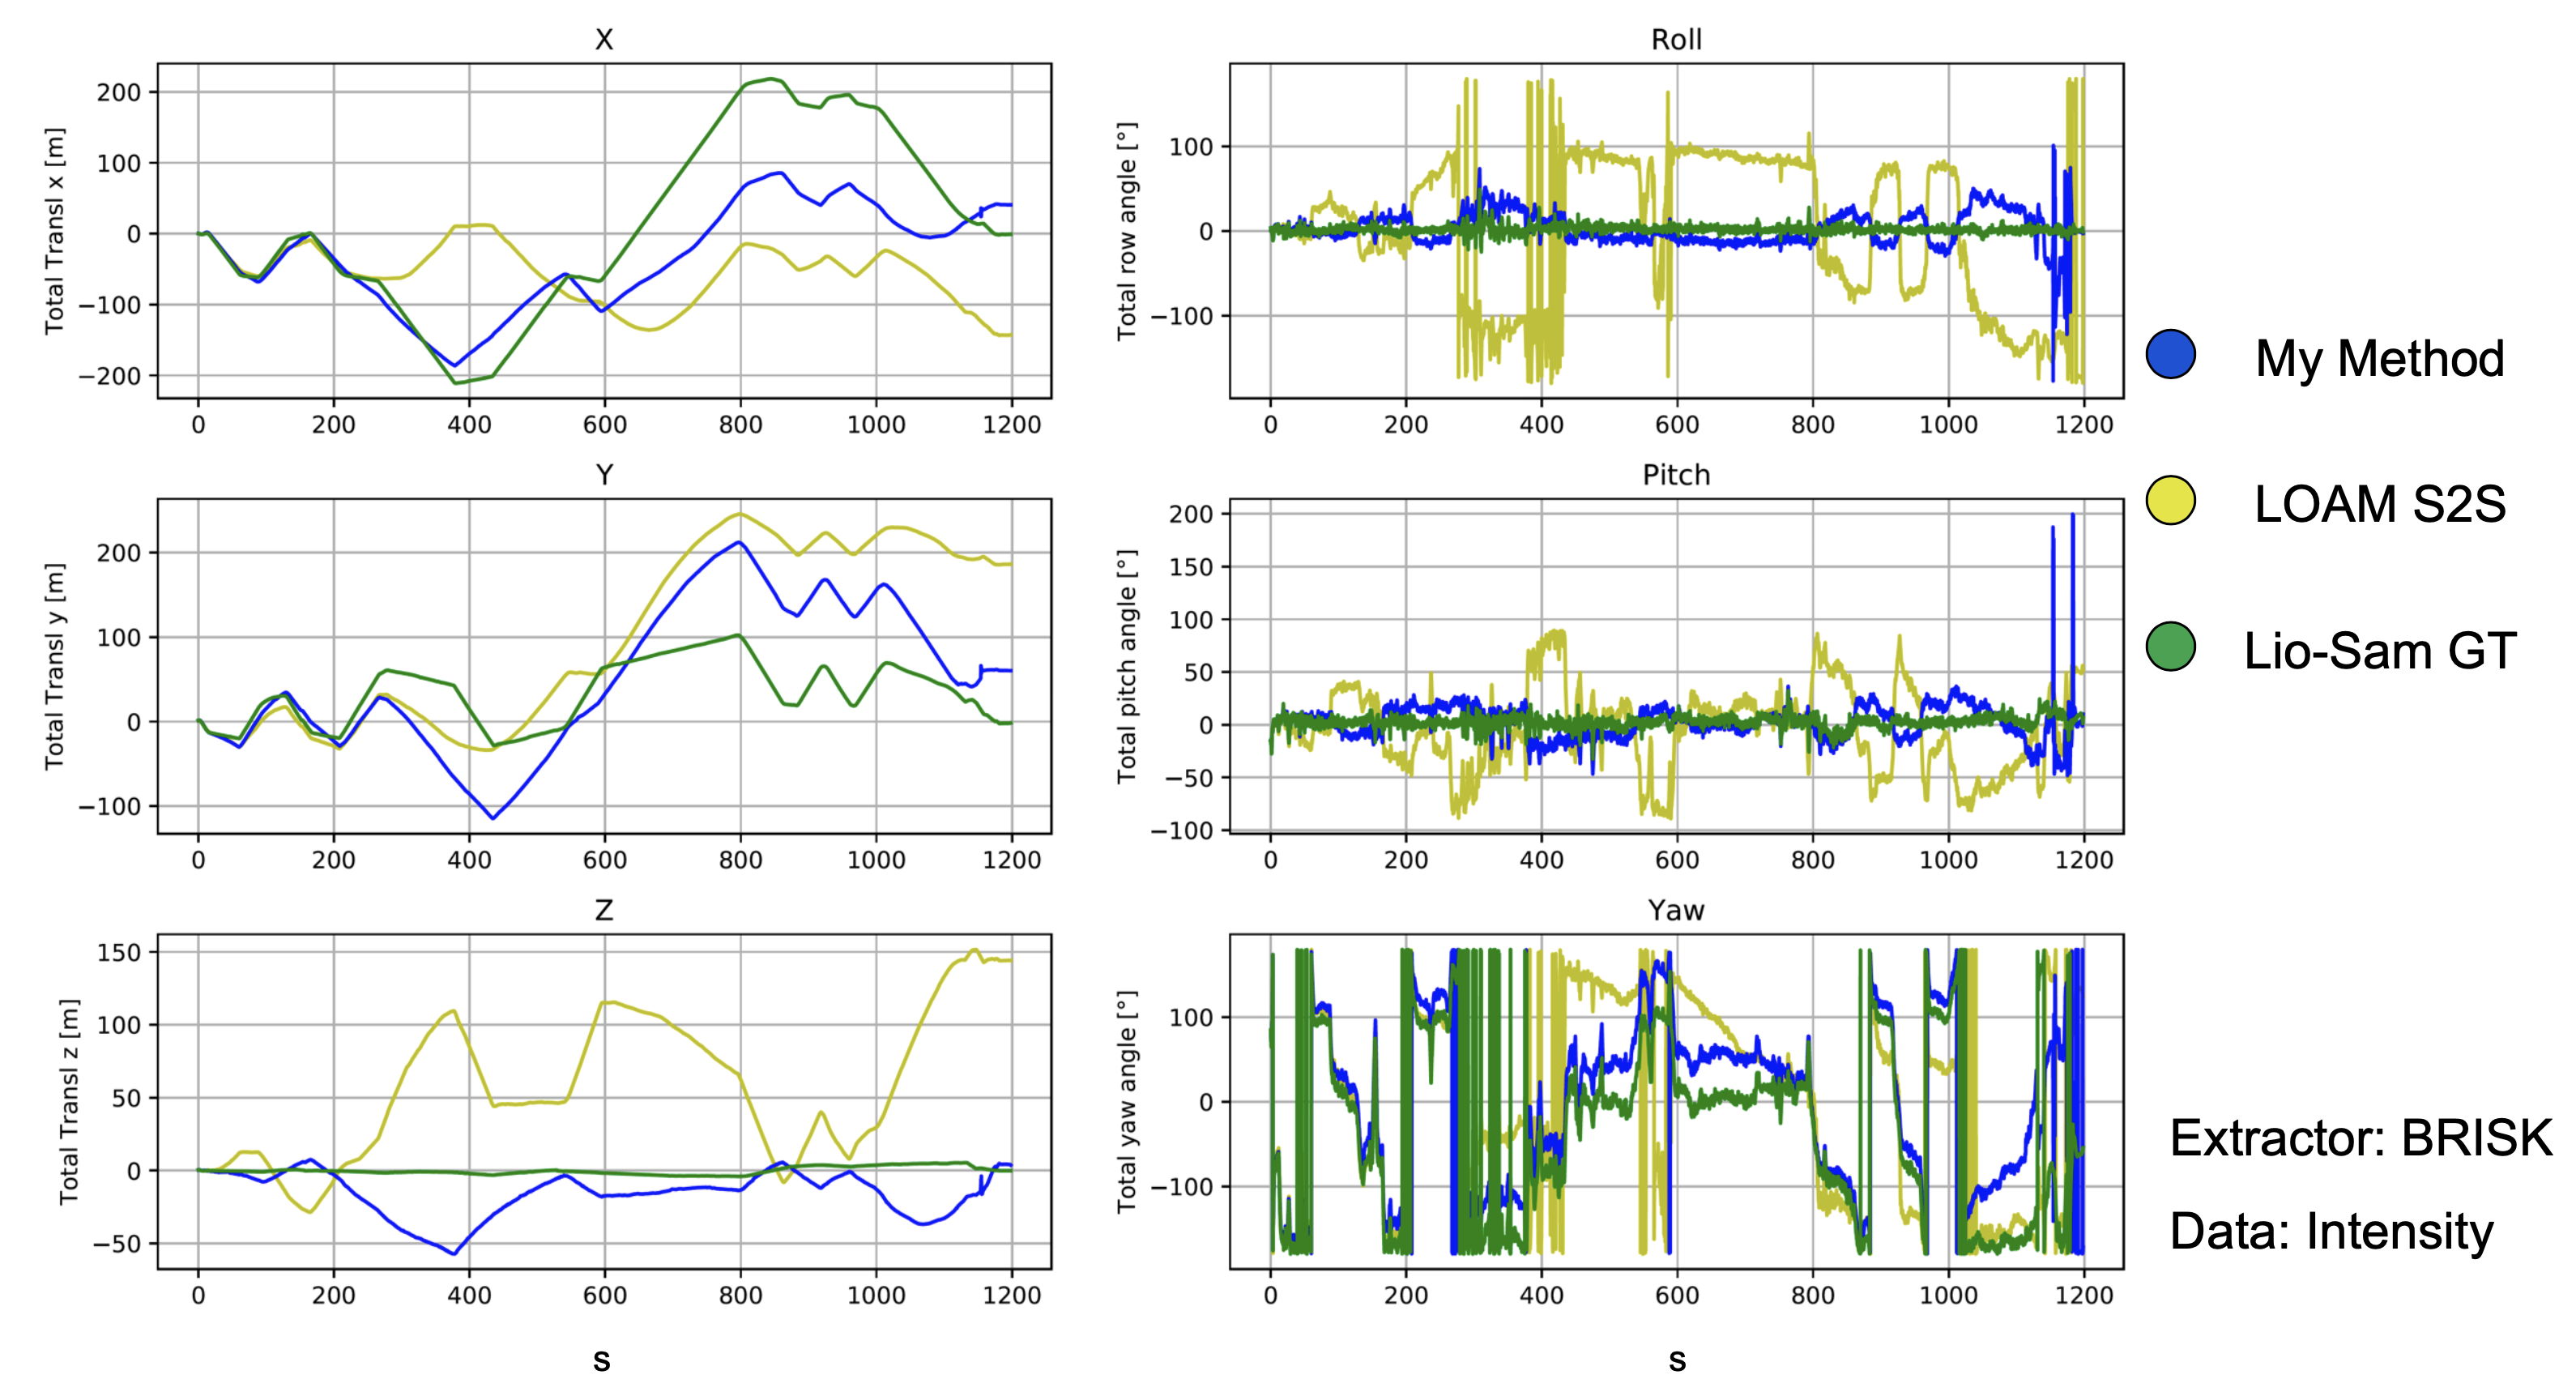
\includegraphics[scale = 0.25]{images/comparison_appendix/pose_brisk.png}
        \caption{Pose comparison brisk}
        \label{fig:pose_comparison_brisk}
    \end{figure}
    
    \begin{figure}[ht]
        \centering
        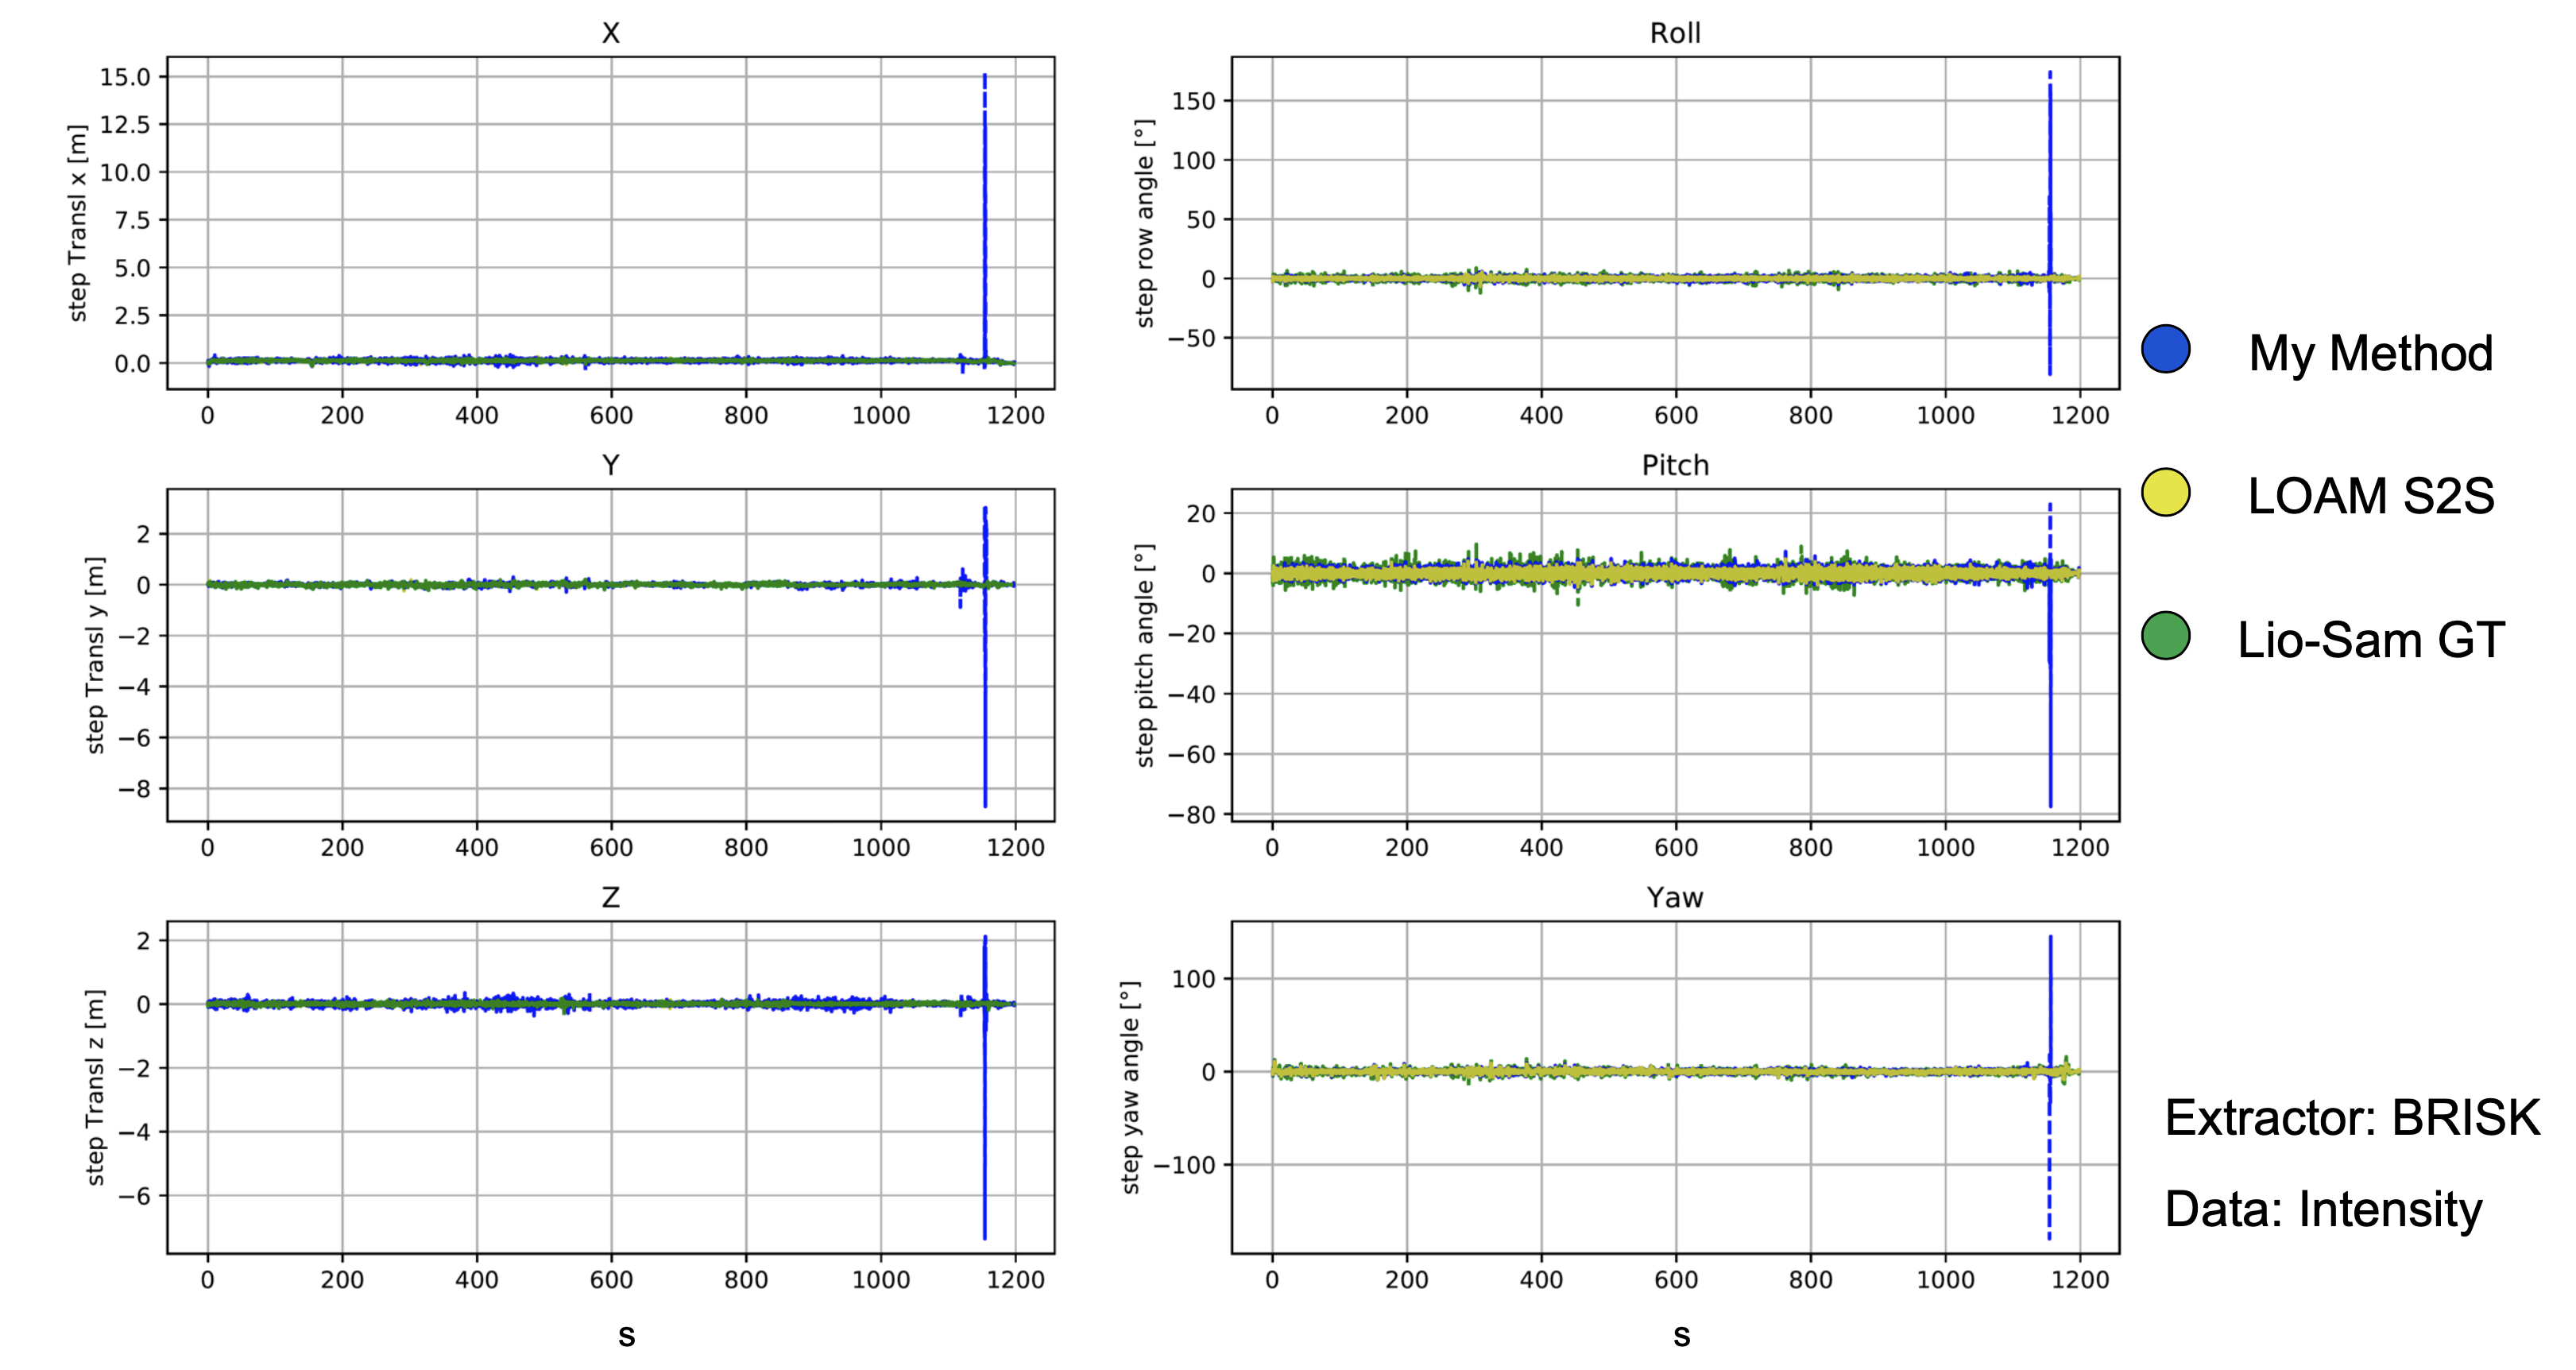
\includegraphics[scale = 0.25]{images/comparison_appendix/steps_brisk.png}
        \caption{Step comparison brisk}
        \label{fig:step_comparison_brisk}
    \end{figure}

    \begin{figure}[ht]
        \centering
        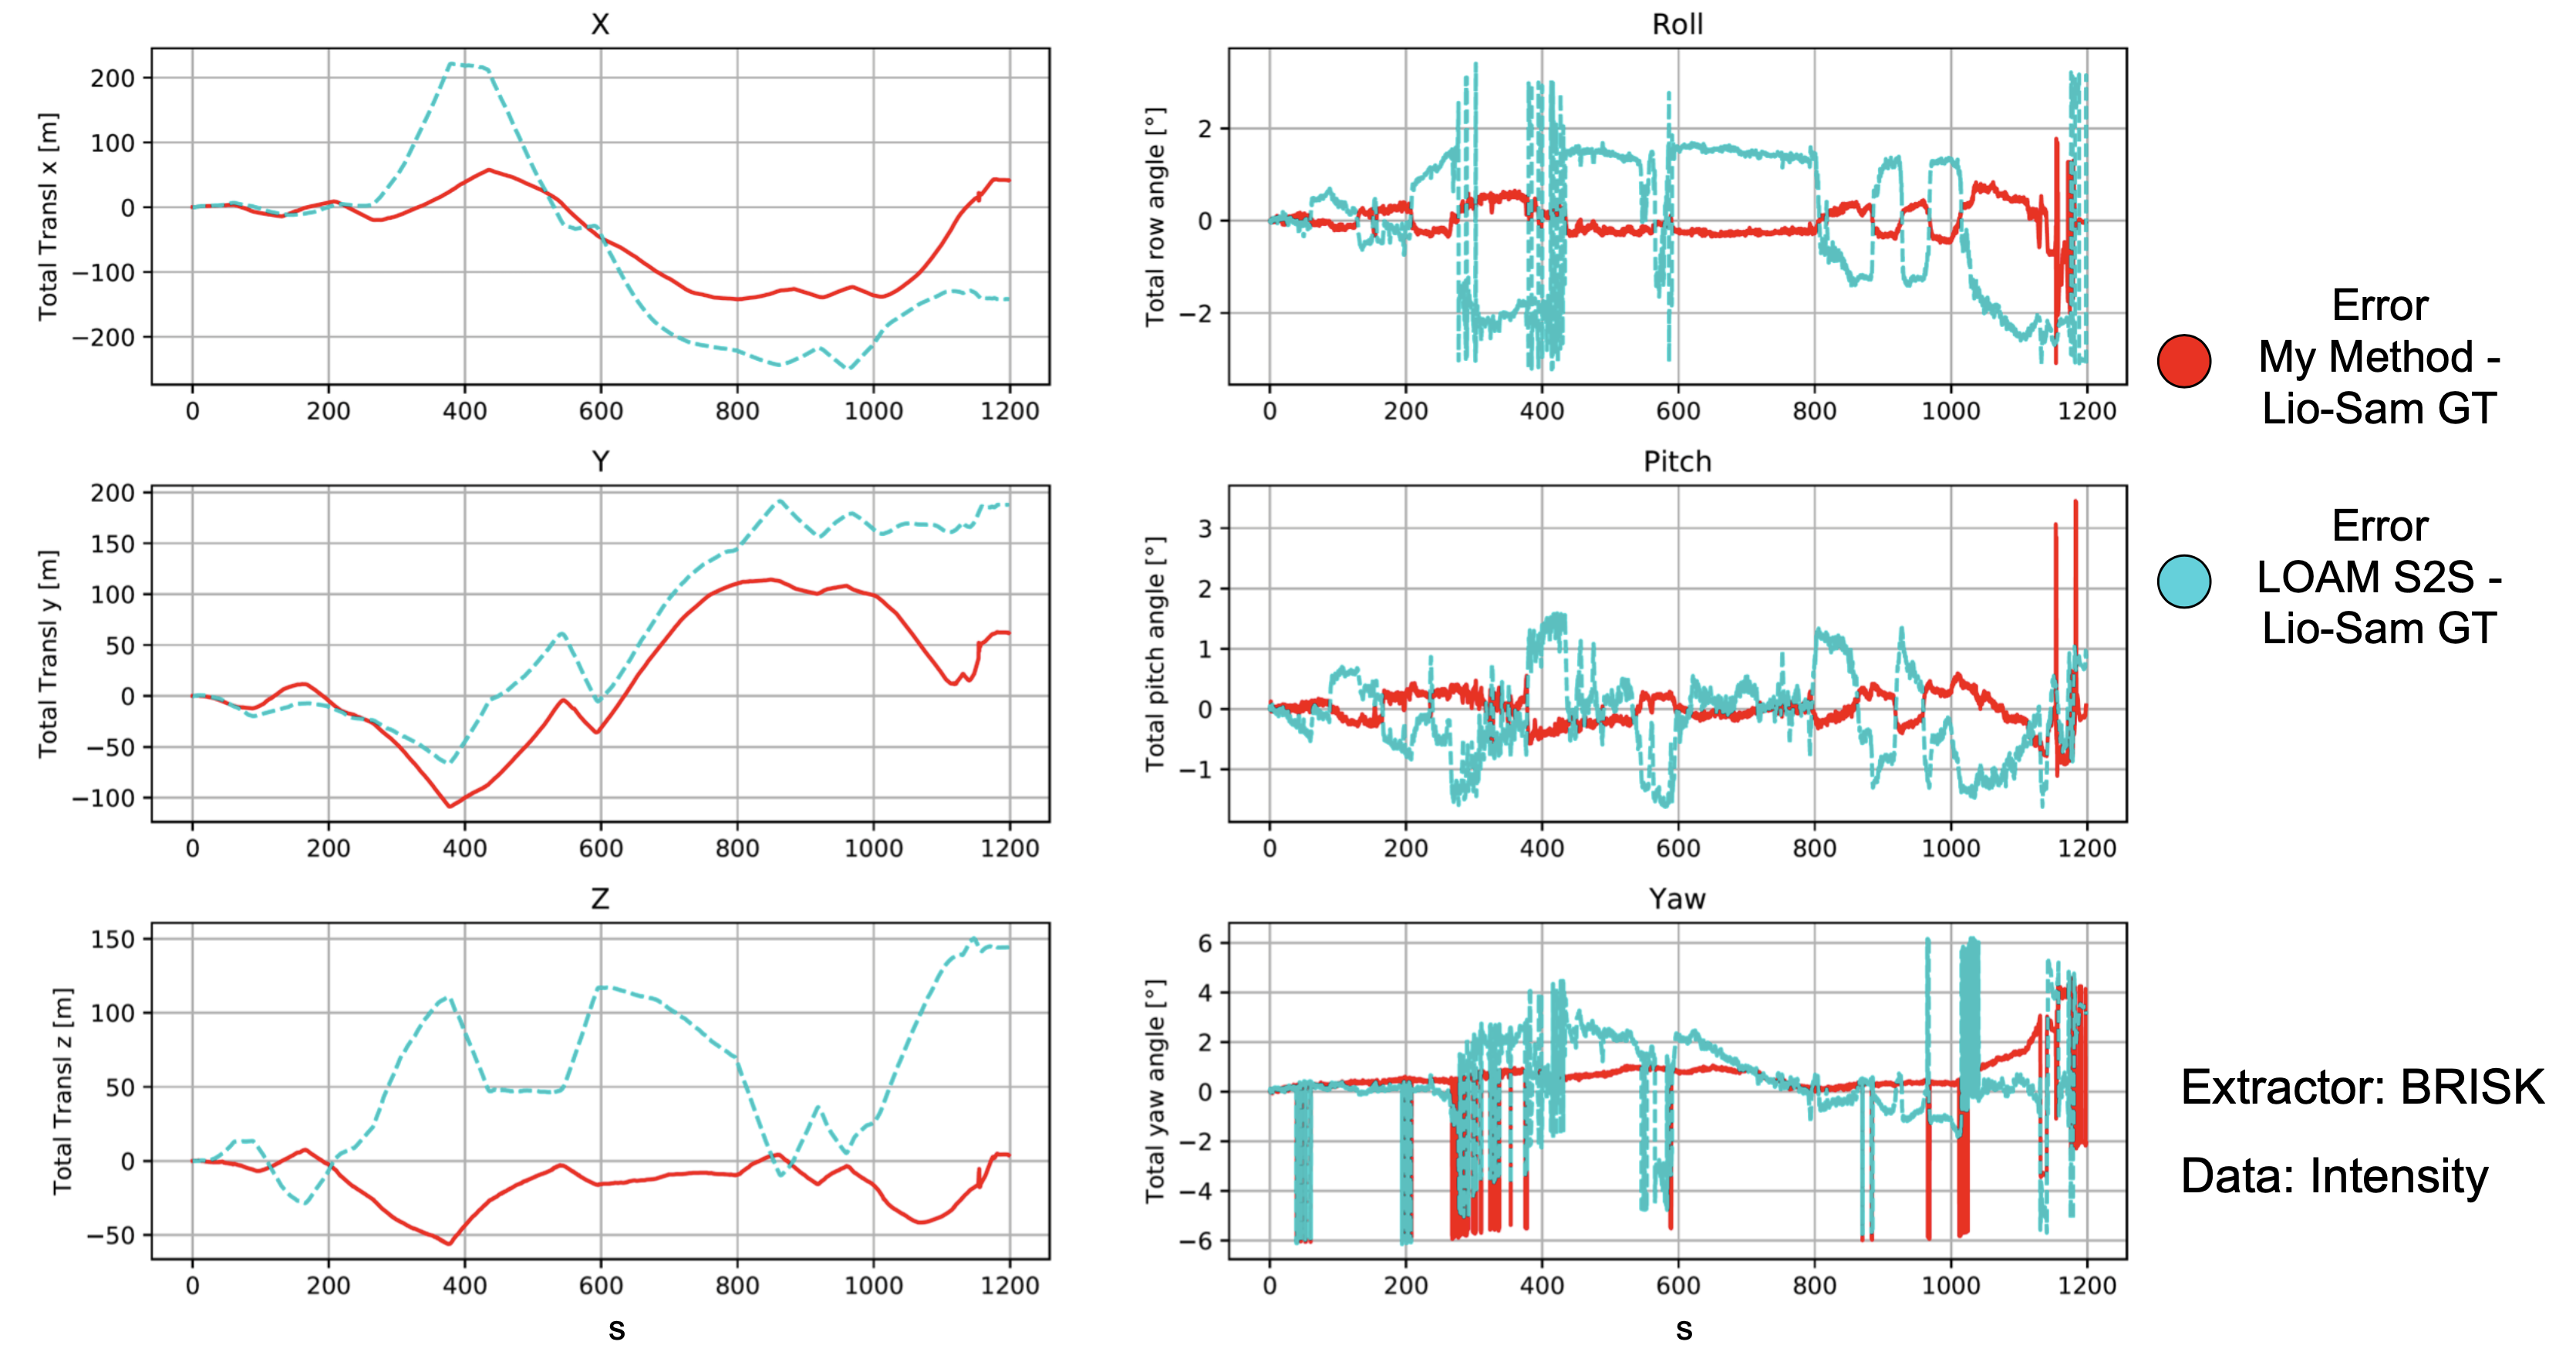
\includegraphics[scale = 0.25]{images/comparison_appendix/pose_error_brisk.png}
        \caption{Pose error comparison brisk}
        \label{fig:pose_error_comparison_brisk}
    \end{figure}
    
    \begin{figure}[ht]
        \centering
        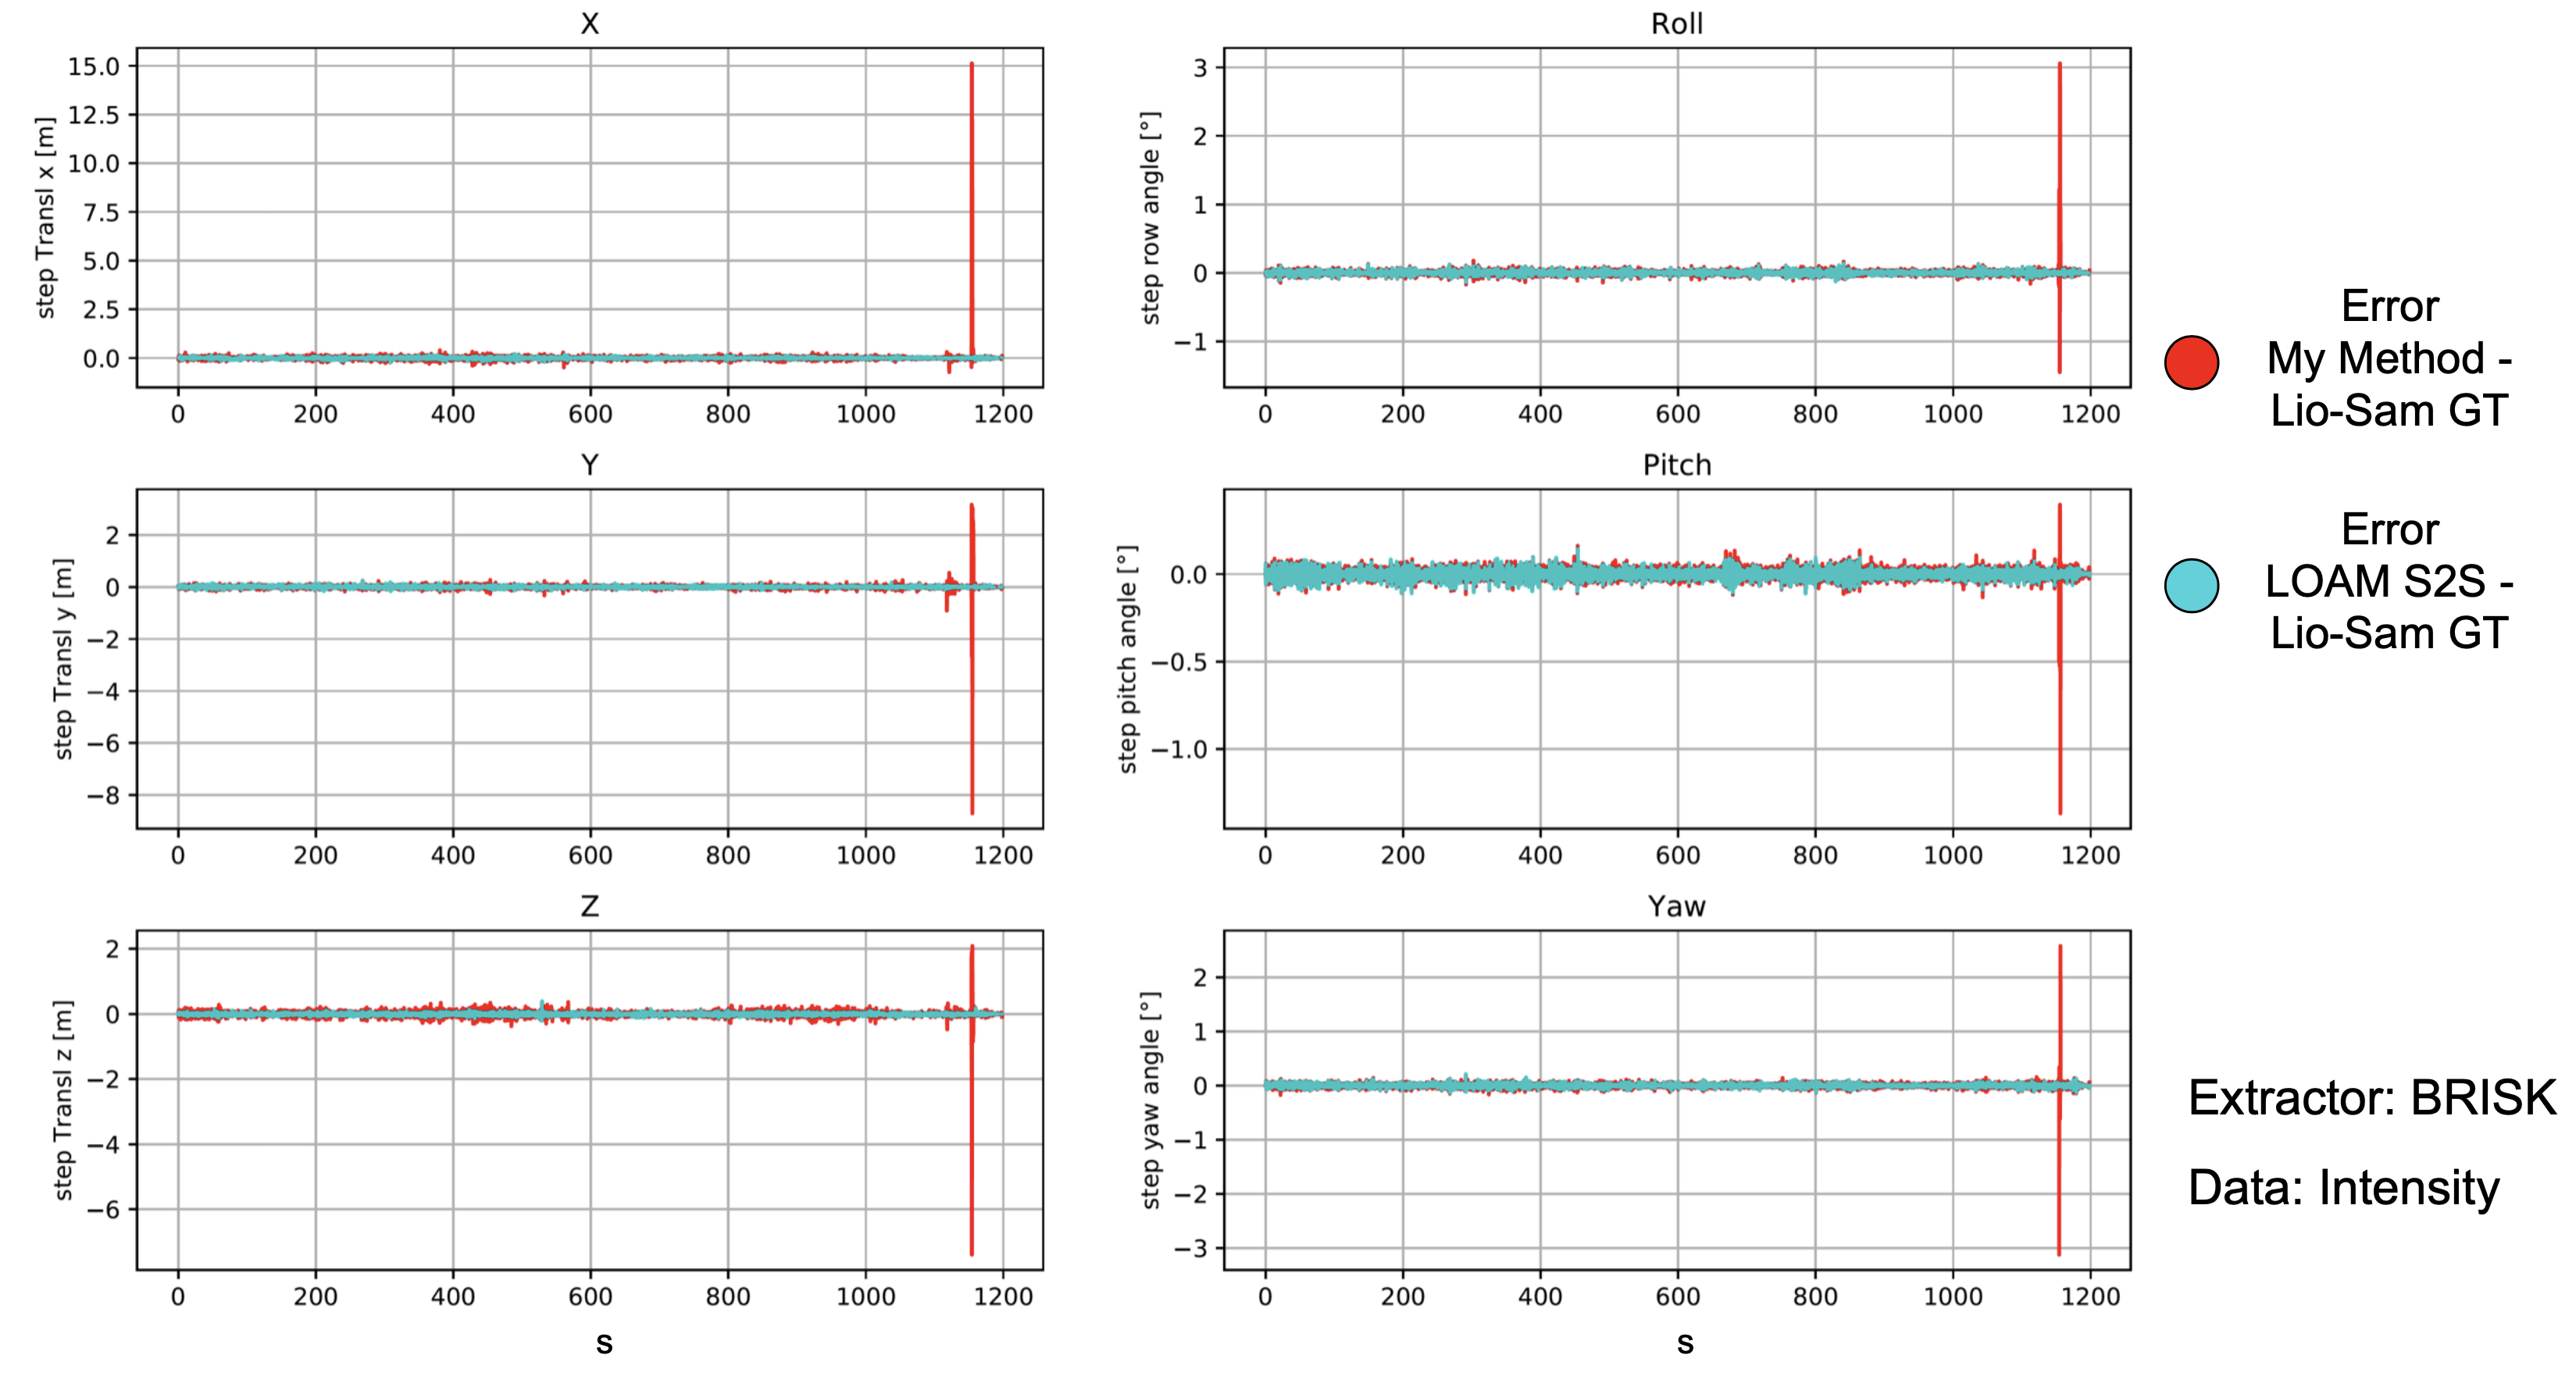
\includegraphics[scale = 0.25]{images/comparison_appendix/step_error_brisk.png}
        \caption{Step error comparison brisk}
        \label{fig:step_error_comparison_brisk}
    \end{figure}
    \clearpage
}

\section{KLT Comparison Plots}{

    \begin{figure}[ht]
        \centering
        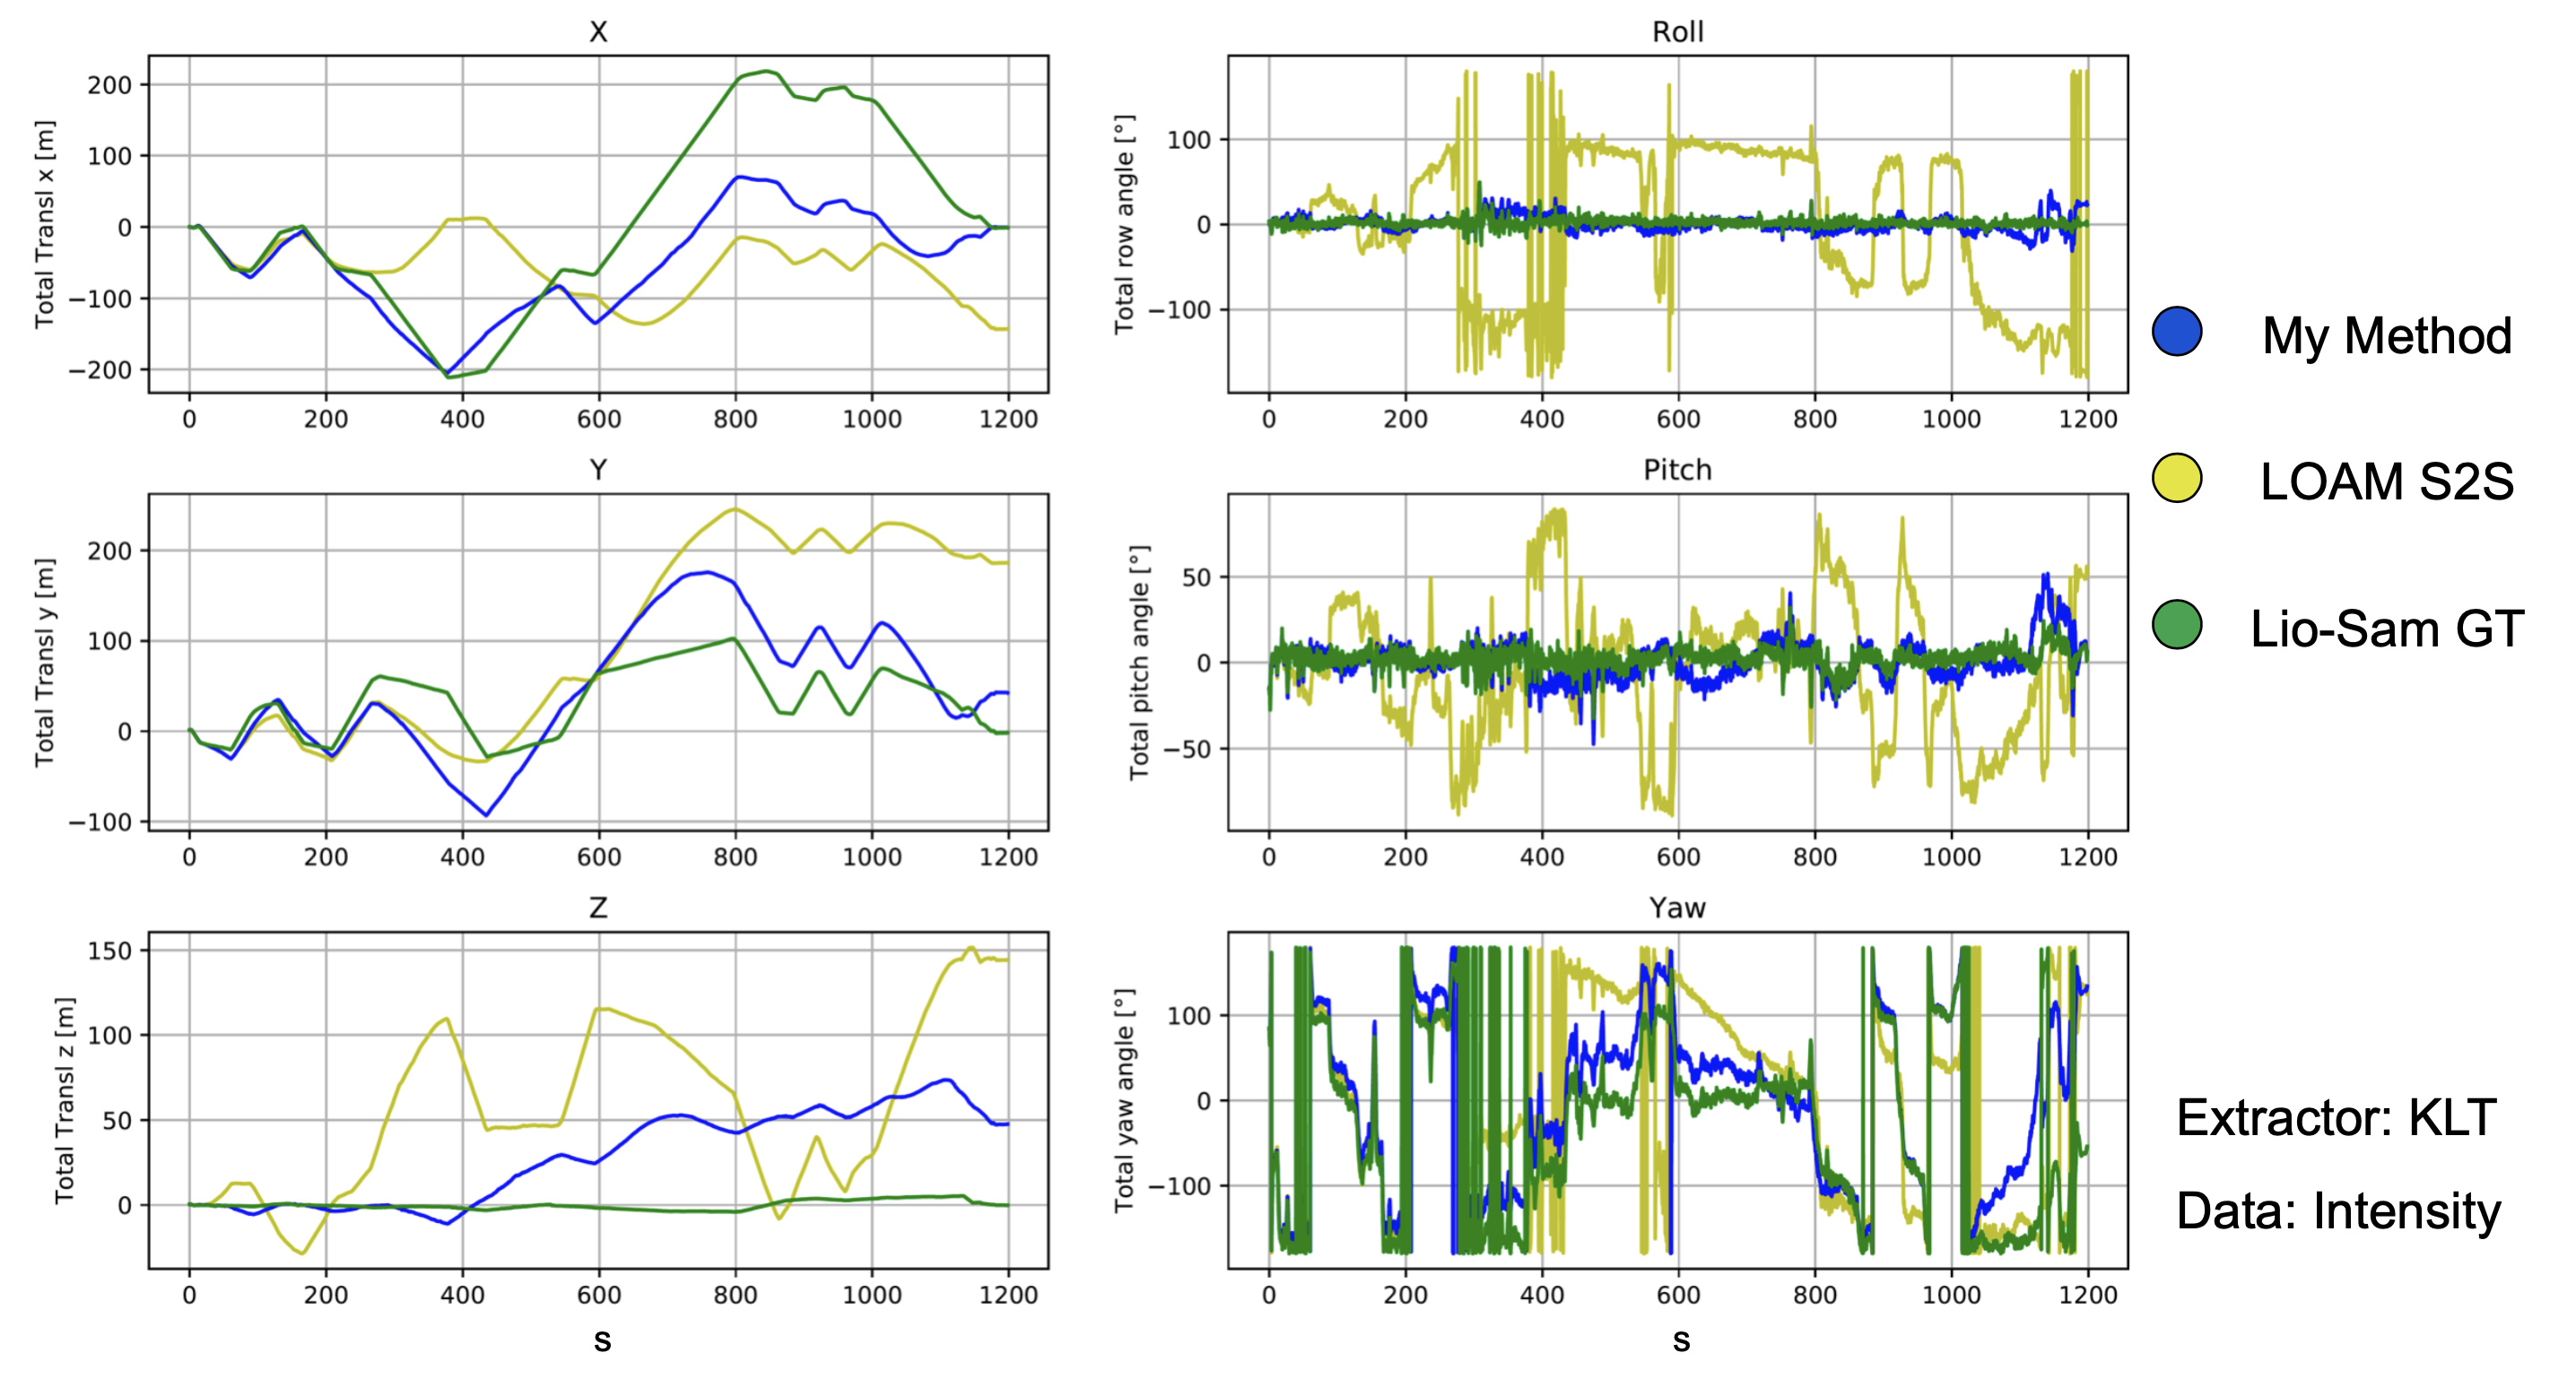
\includegraphics[scale = 0.25]{images/results/pose_klt.png}
        \caption{Pose comparison klt}
        \label{fig:pose_comparison_klt_appendix}
    \end{figure}
    
    \begin{figure}[ht]
        \centering
        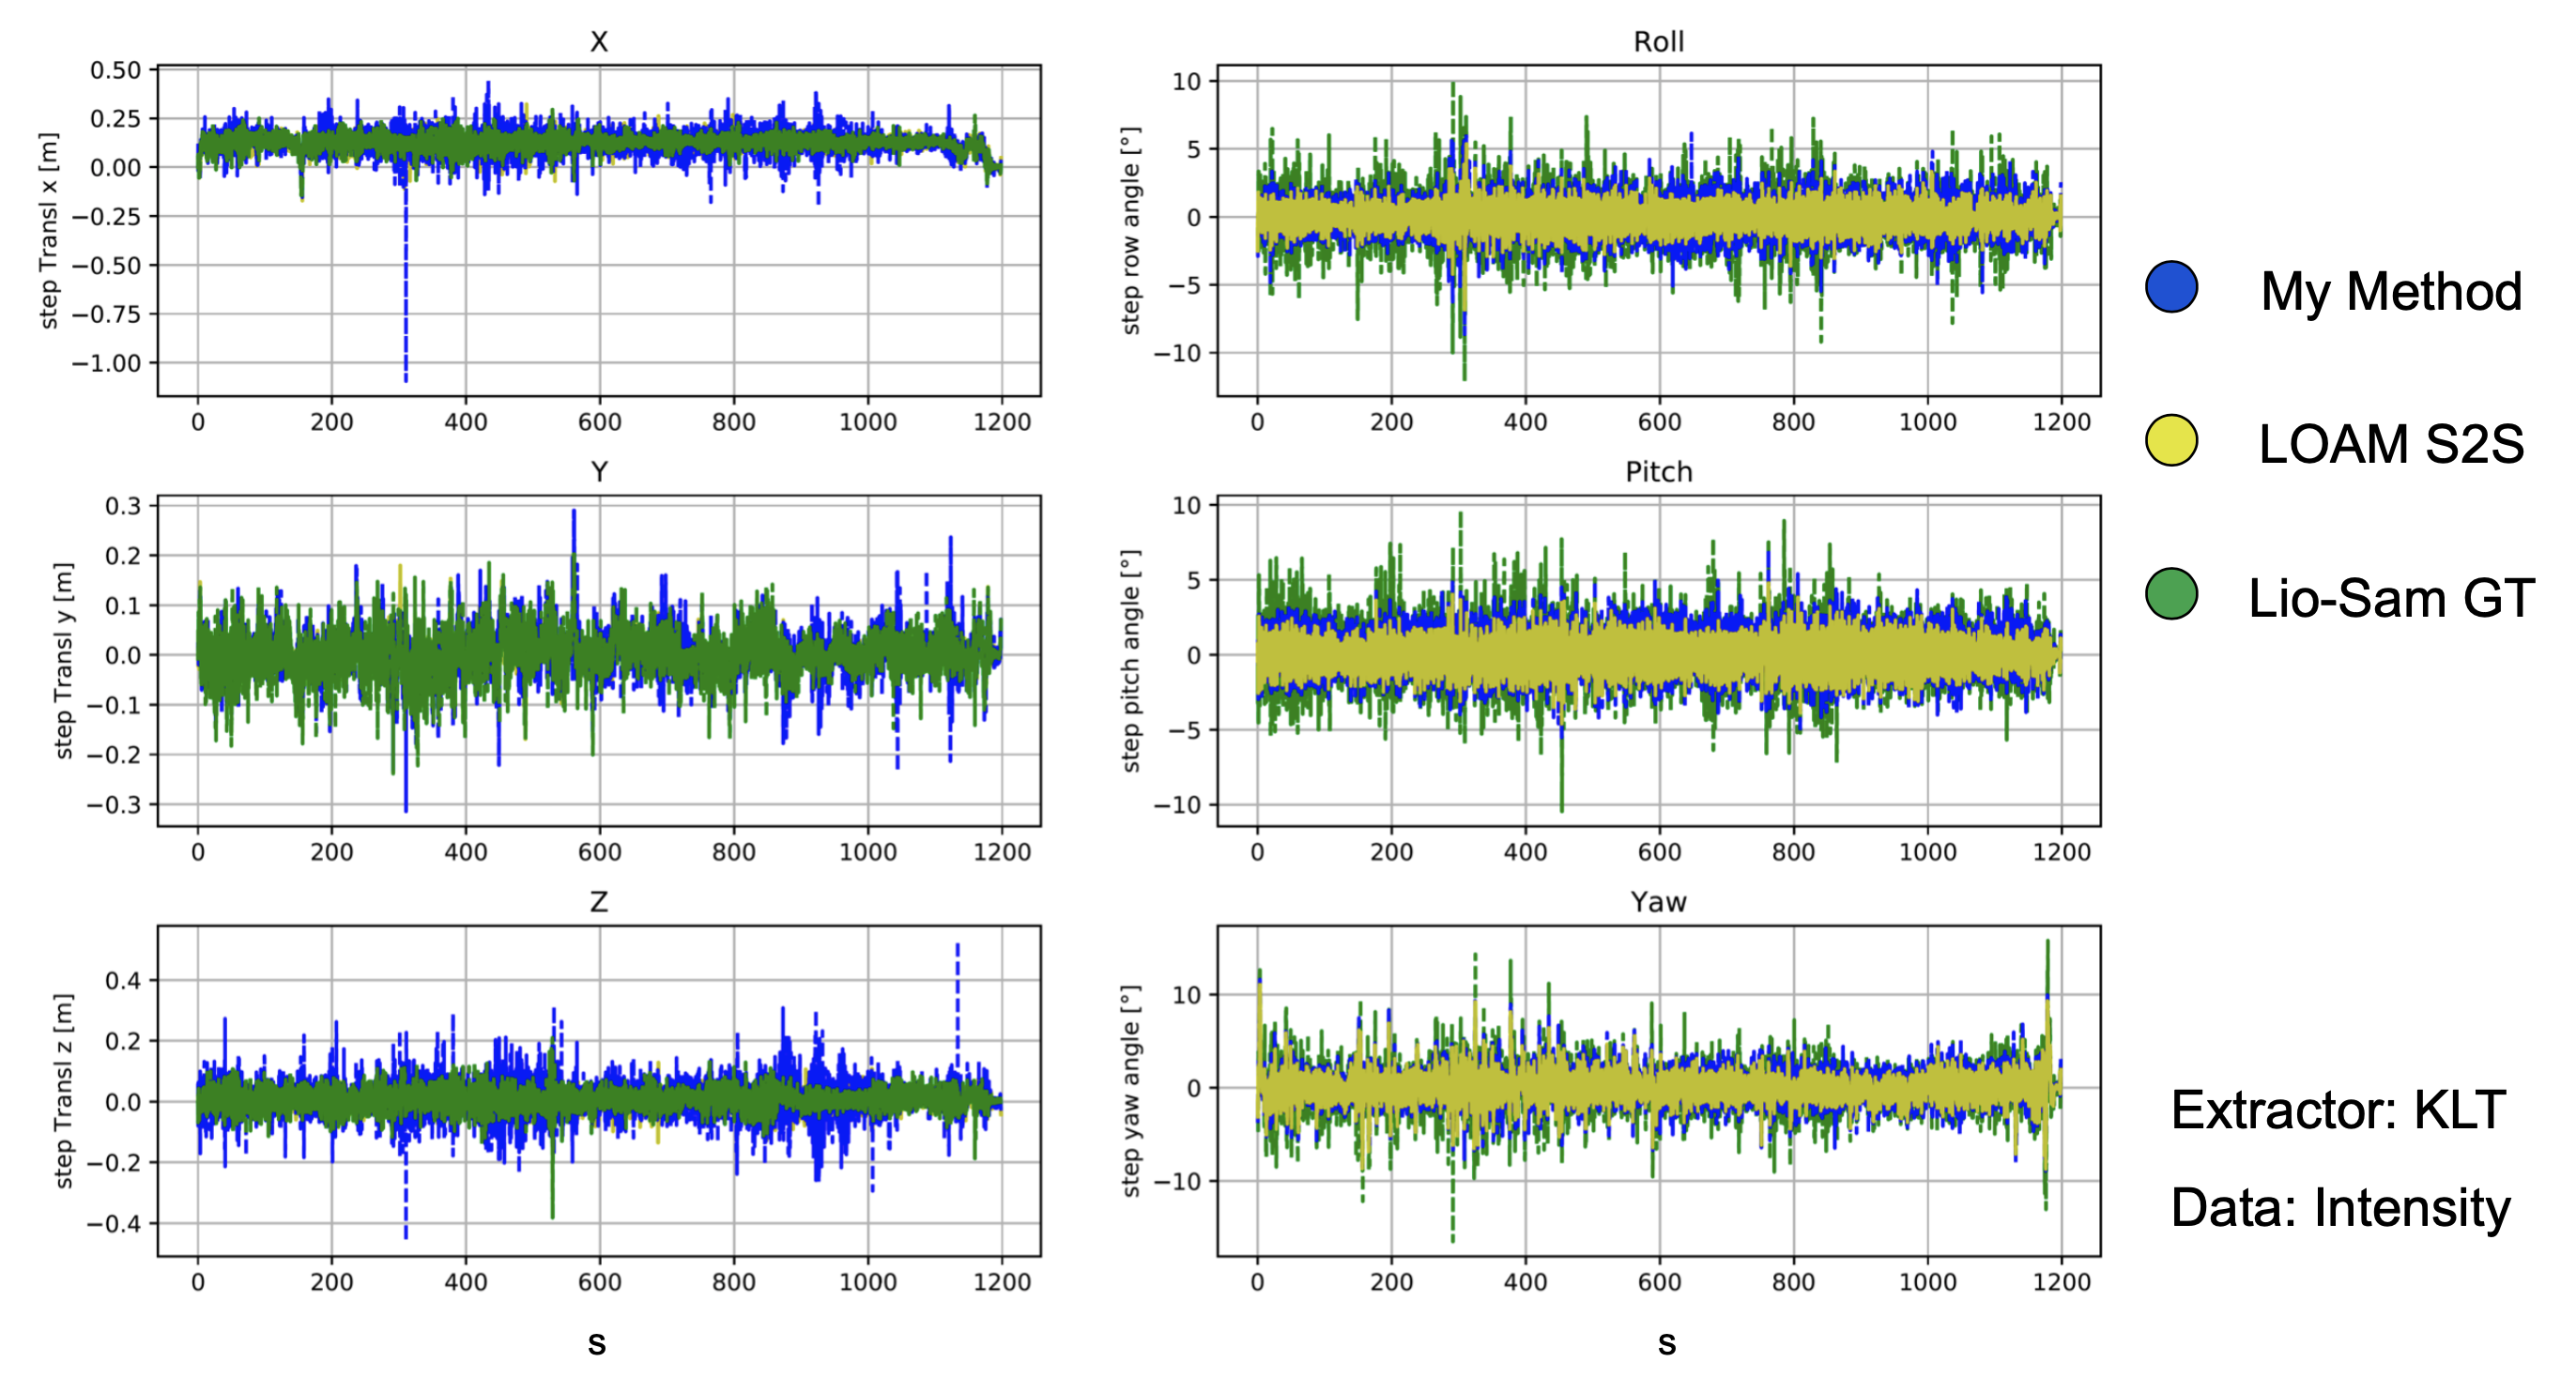
\includegraphics[scale = 0.25]{images/results/steps_klt.png}
        \caption{Step comparison klt}
        \label{fig:step_comparison_klt_appendix}
    \end{figure}

    \begin{figure}[ht]
        \centering
        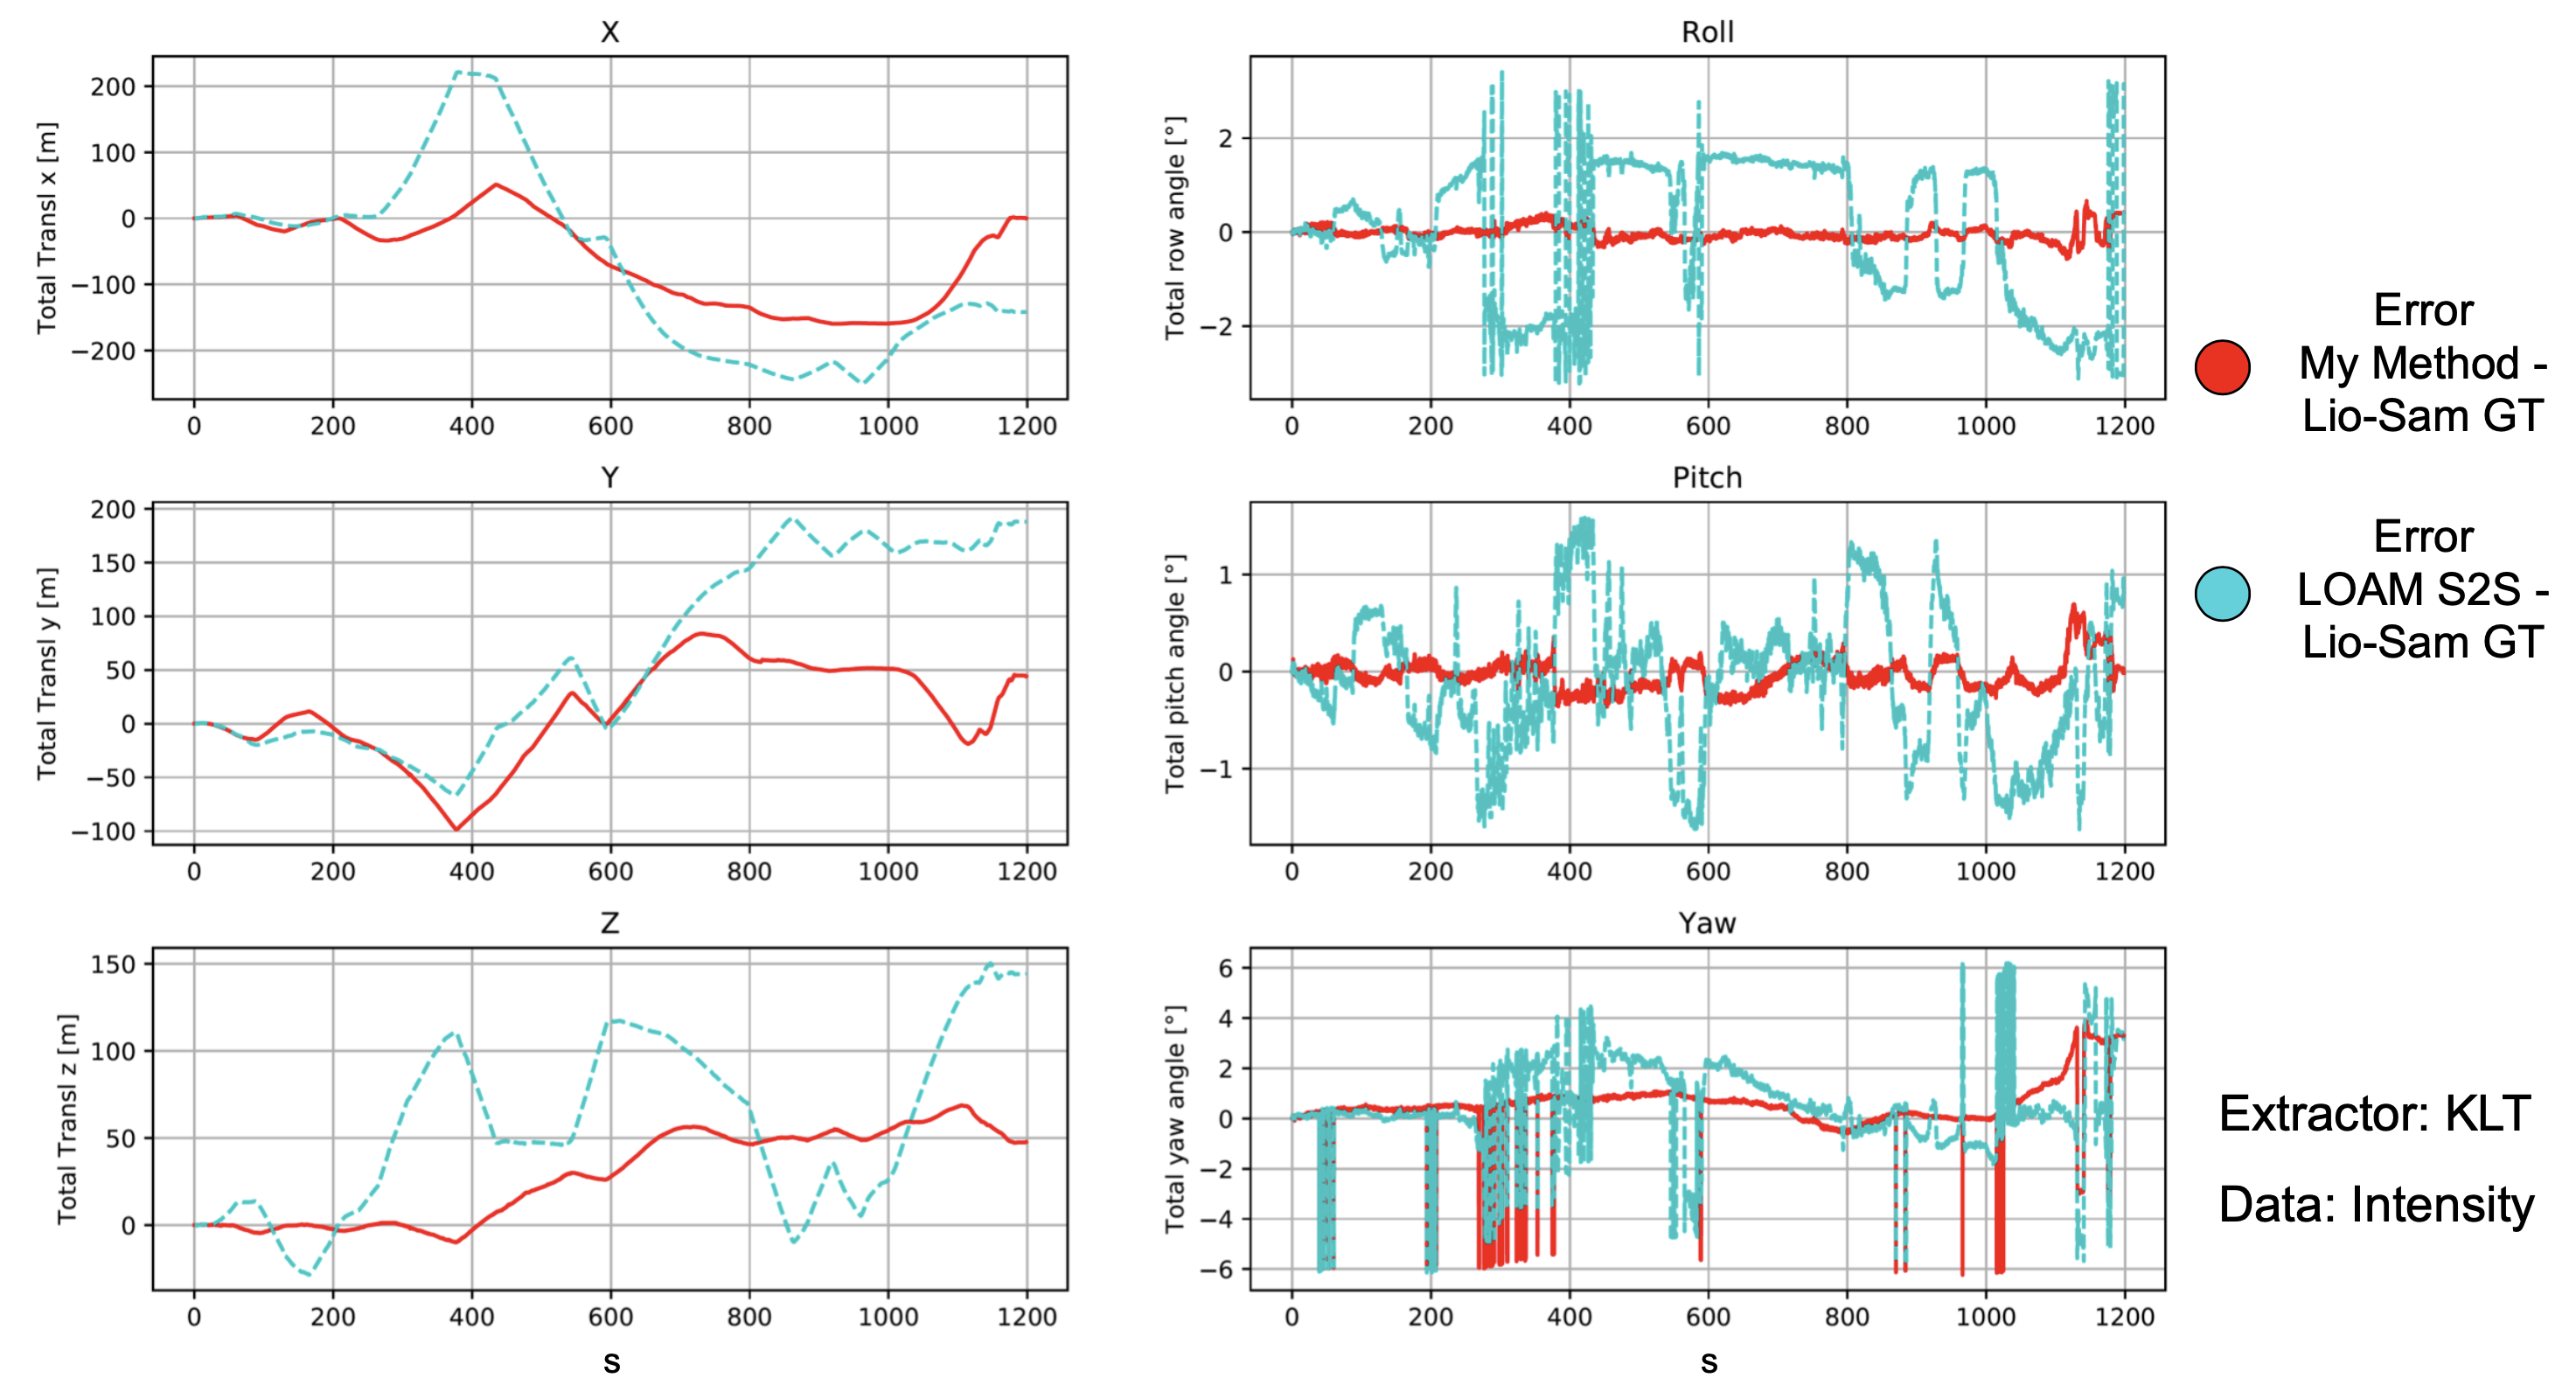
\includegraphics[scale = 0.25]{images/results/pose_error_klt.png}
        \caption{Pose error comparison klt}
        \label{fig:pose_error_comparison_klt_appendix}
    \end{figure}
    
    \begin{figure}[ht]
        \centering
        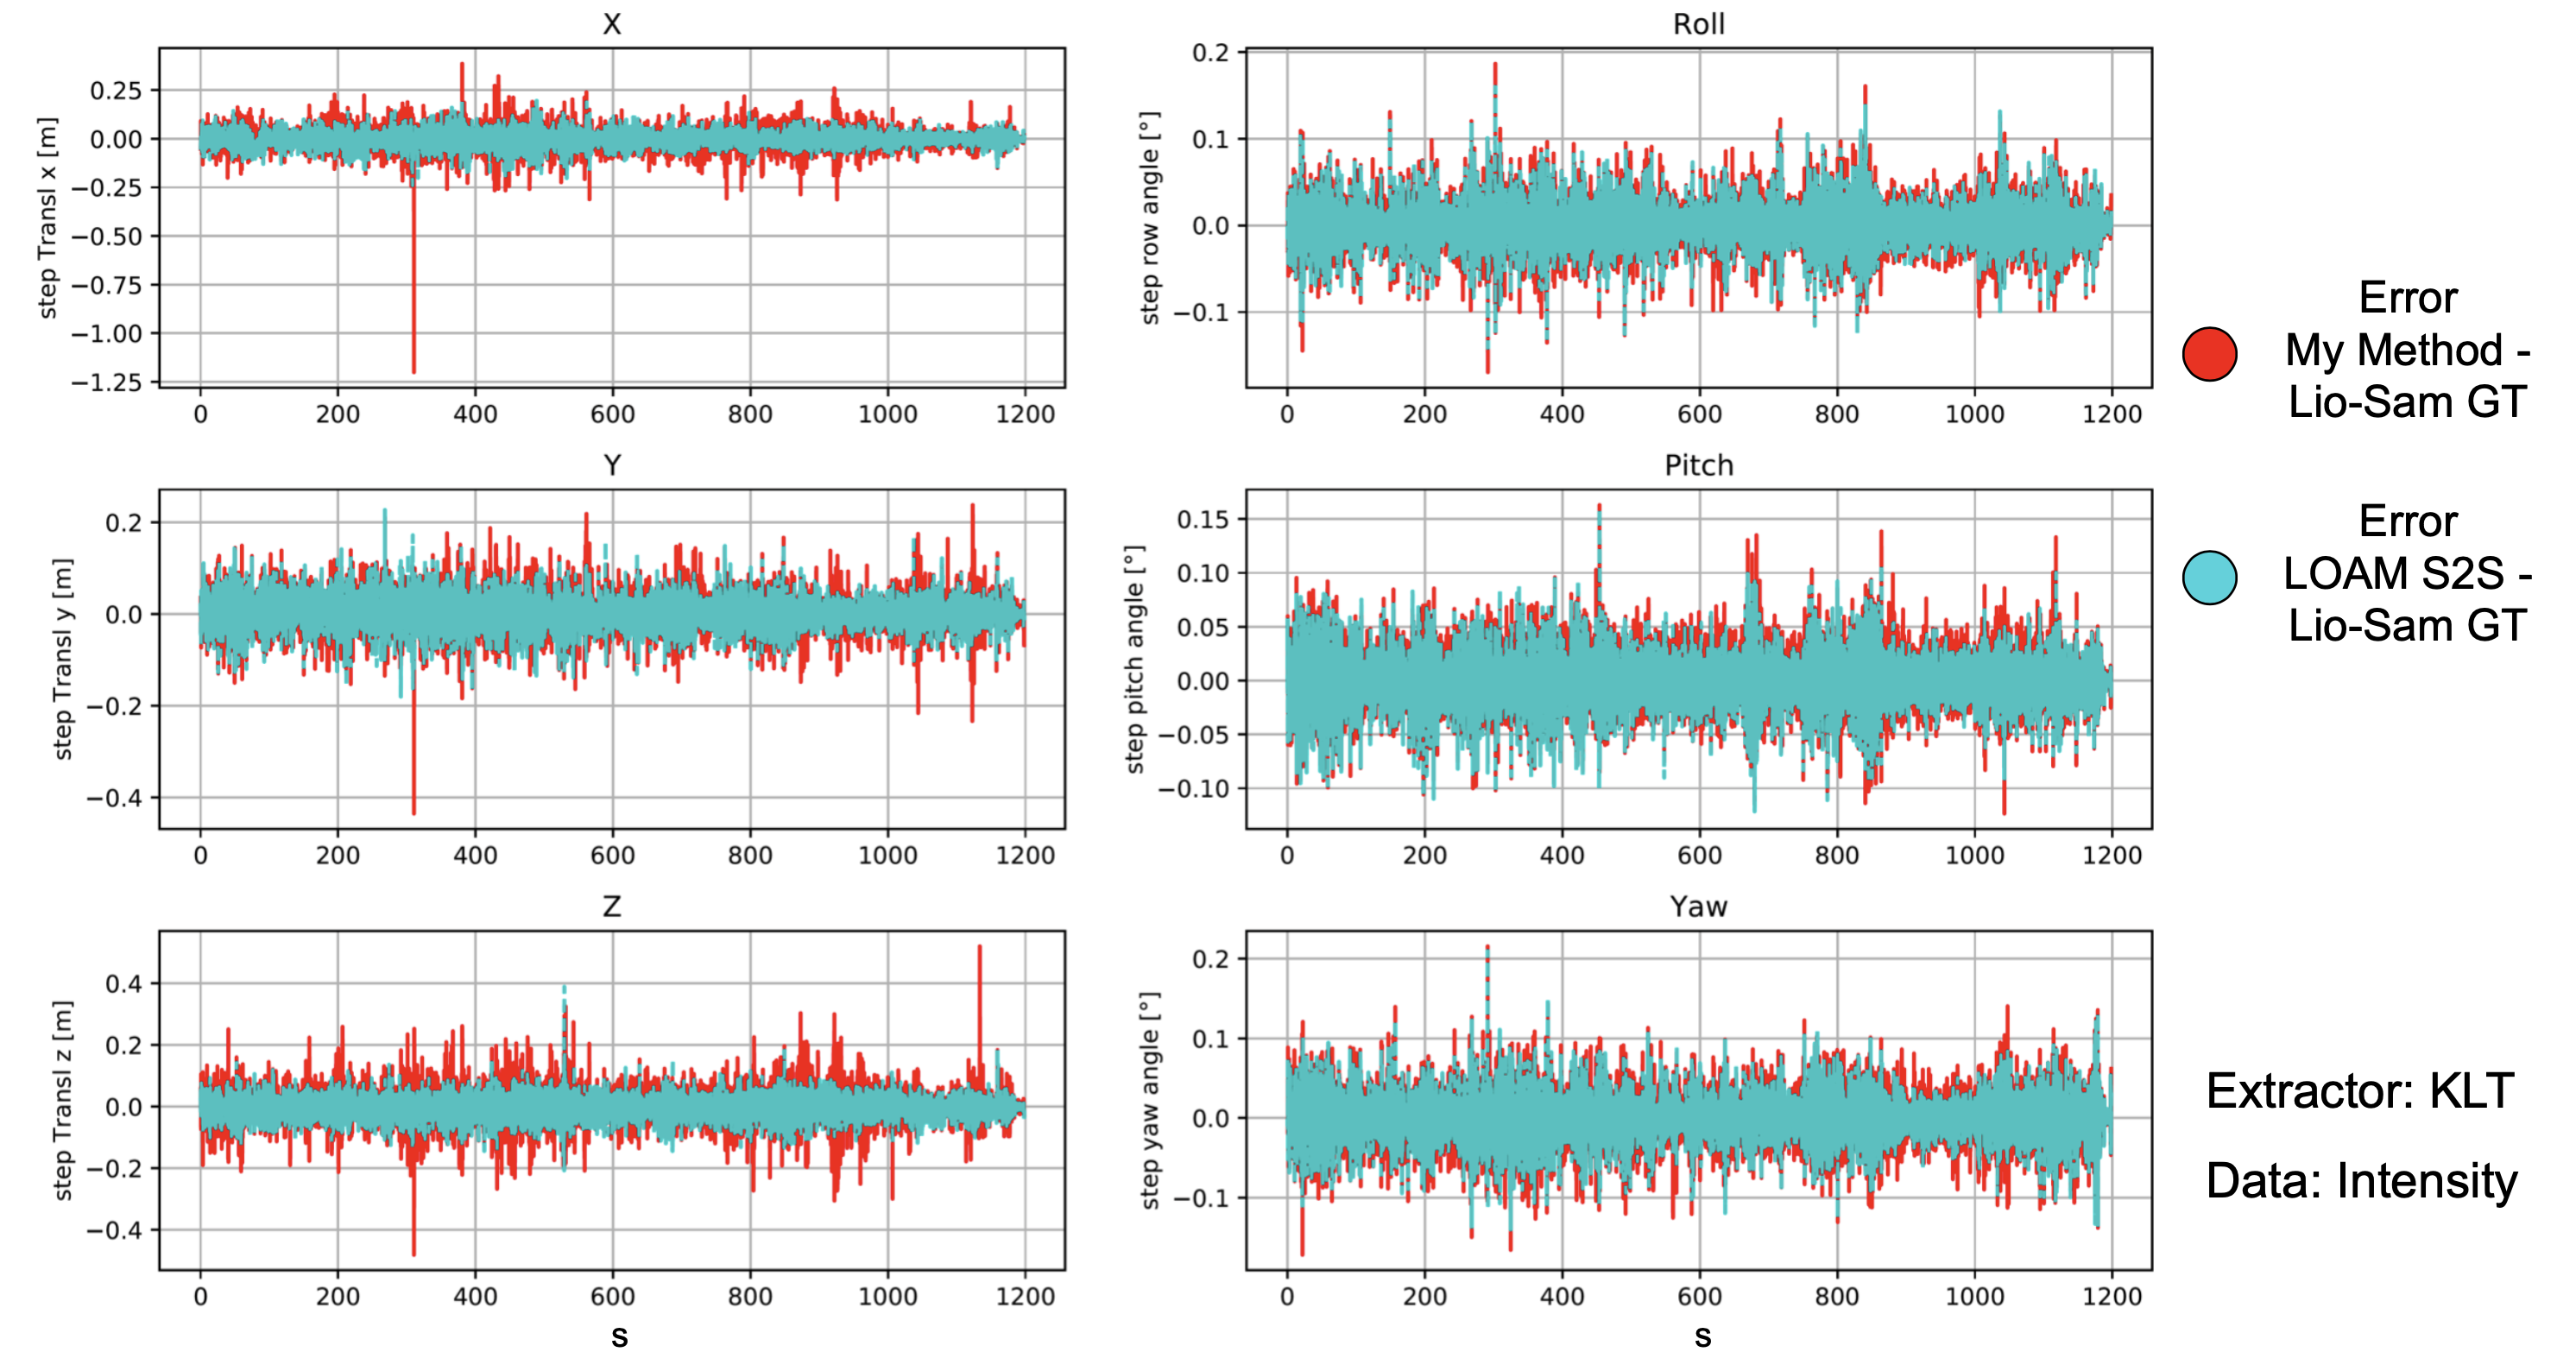
\includegraphics[scale = 0.25]{images/results/step_error_klt.png}
        \caption{Step error comparison klt}
        \label{fig:step_error_comparison_klt_appendix}
    \end{figure}
    \clearpage
}



\section{Intensity Data Comparison Plots}{
    For the intensity data consider \cref{sec:ORBcomp} as the comparison base was intensity and ORB and they are thus the same.
}
\section{Ambient Data Comparison Plots}{

    \begin{figure}[ht]
        \centering
        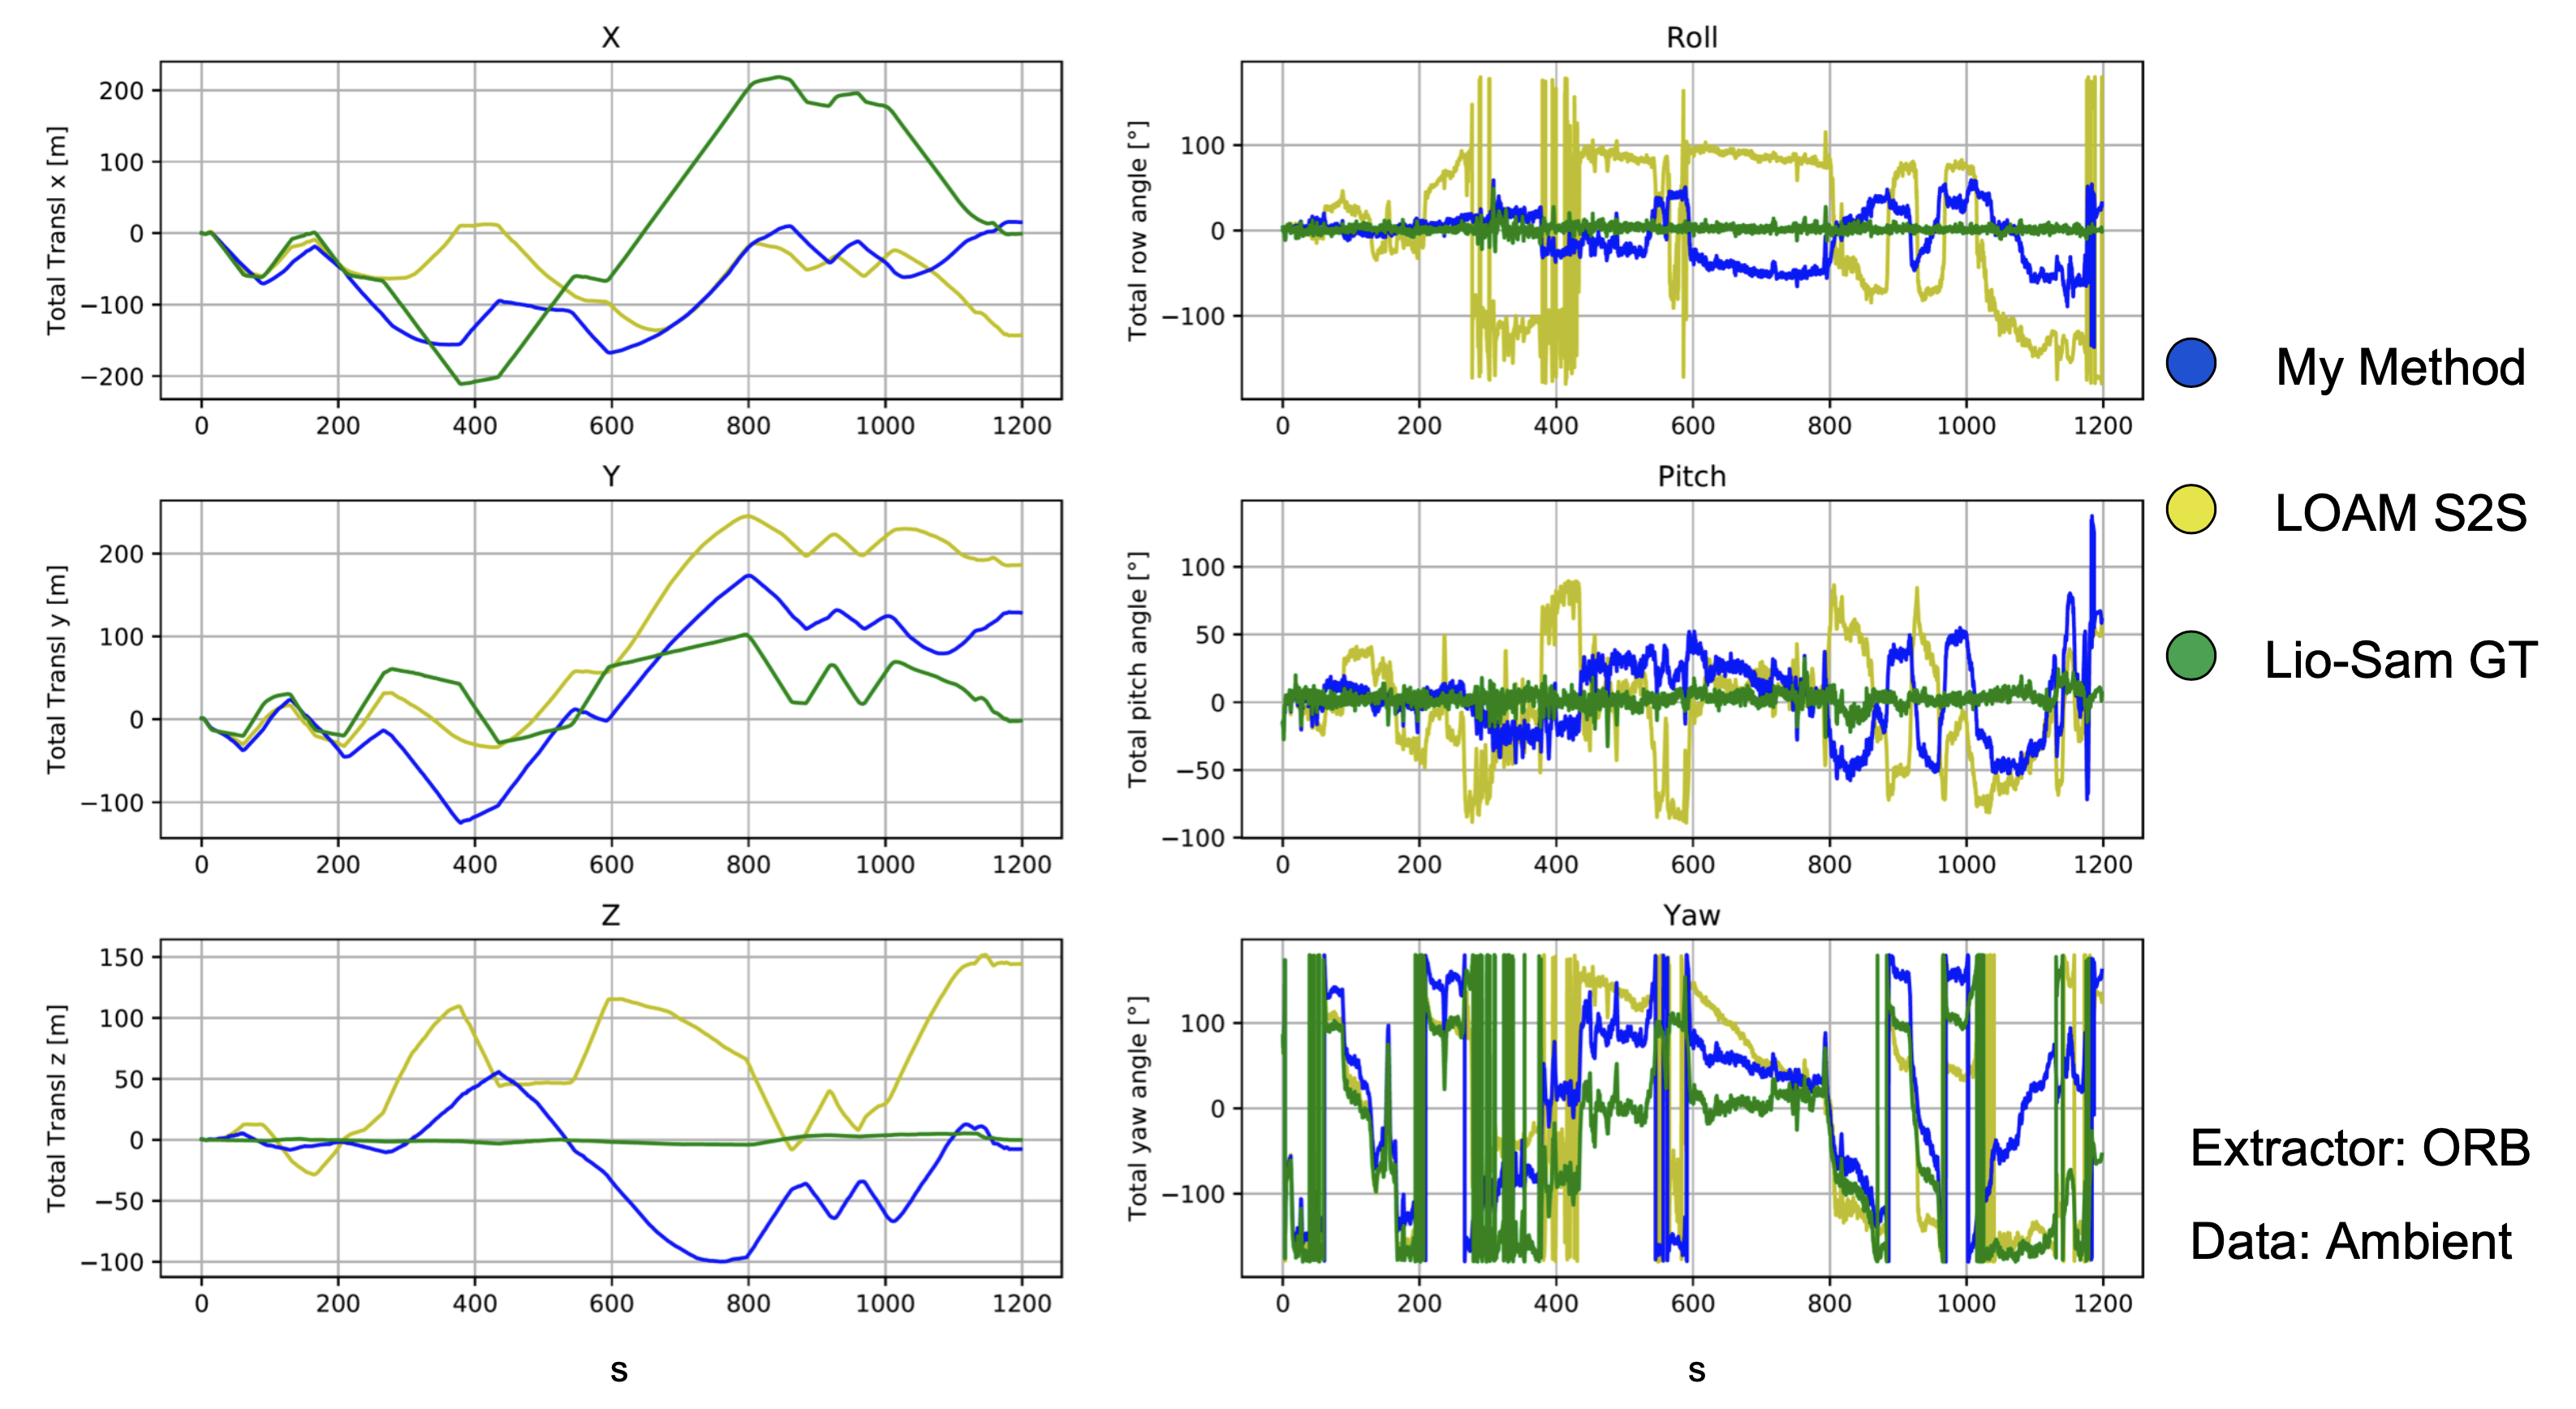
\includegraphics[scale = 0.25]{images/comparison_appendix/pose_ambient.png}
        \caption{Pose comparison ambient}
        \label{fig:pose_comparison_ambient}
    \end{figure}
    
    \begin{figure}[ht]
        \centering
        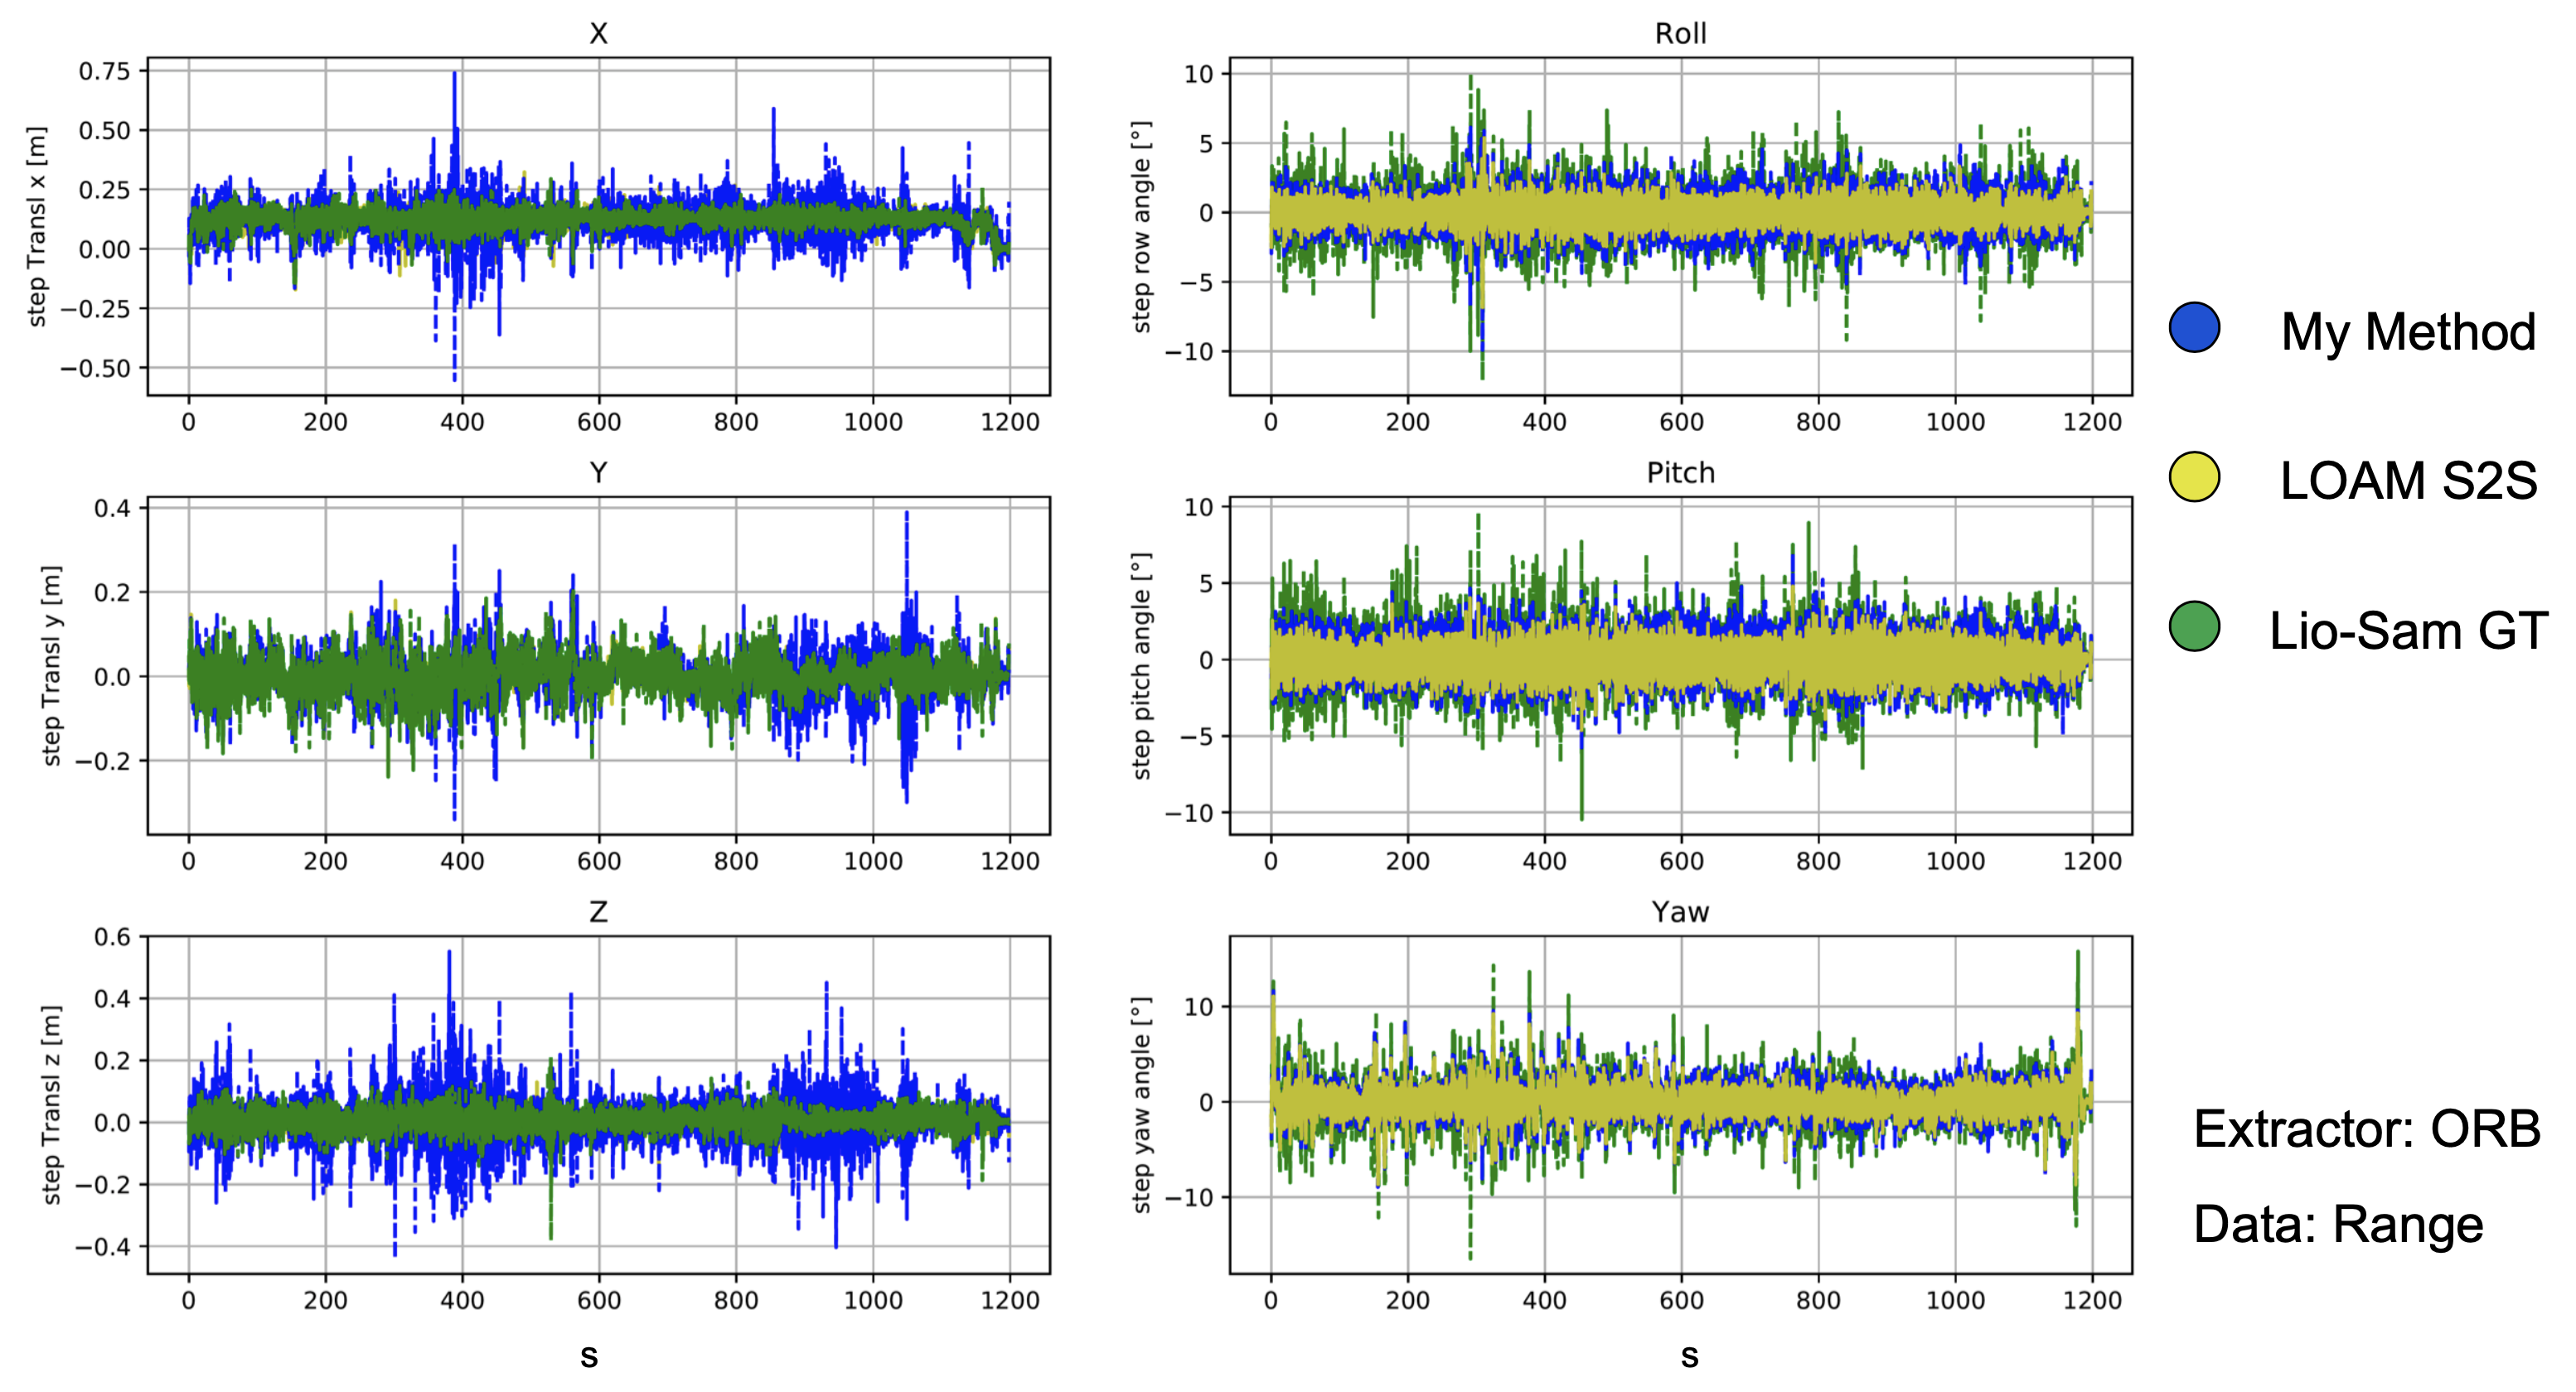
\includegraphics[scale = 0.25]{images/comparison_appendix/steps_ambient.png}
        \caption{Step comparison ambient}
        \label{fig:step_comparison_ambient}
    \end{figure}

    \begin{figure}[ht]
        \centering
        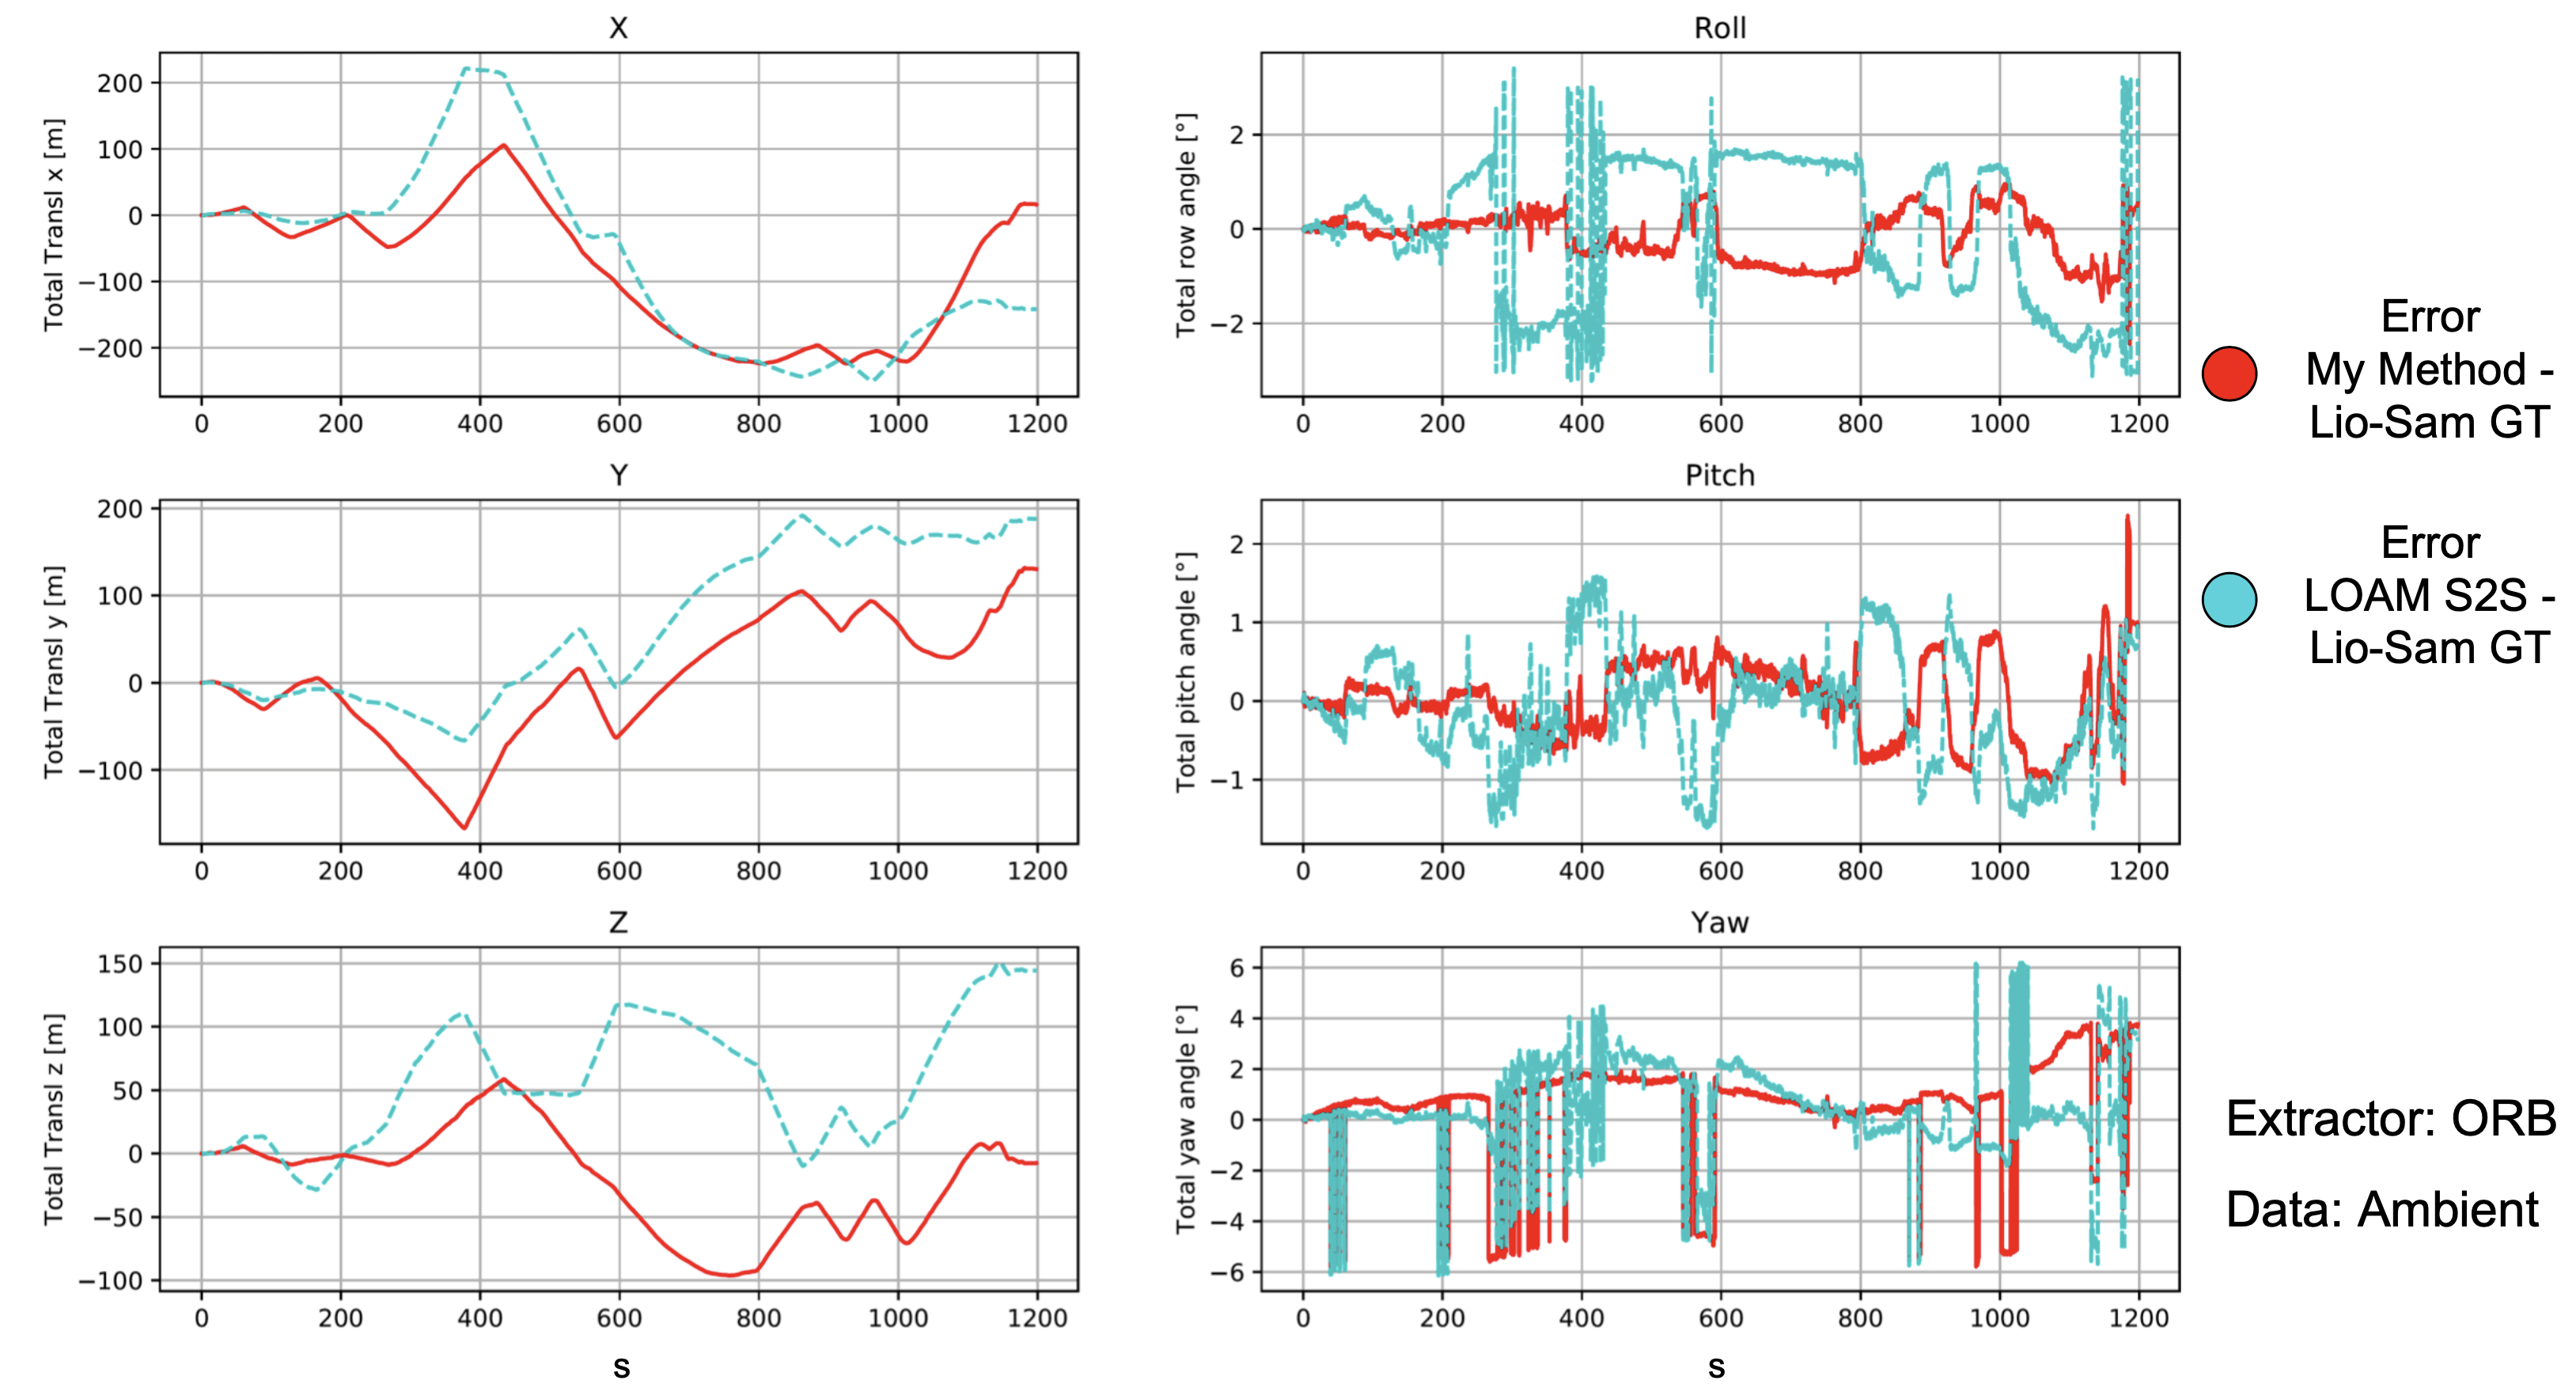
\includegraphics[scale = 0.25]{images/comparison_appendix/pose_error_ambient.png}
        \caption{Pose error comparison ambient}
        \label{fig:pose_error_comparison_ambient}
    \end{figure}
    
    \begin{figure}[ht]
        \centering
        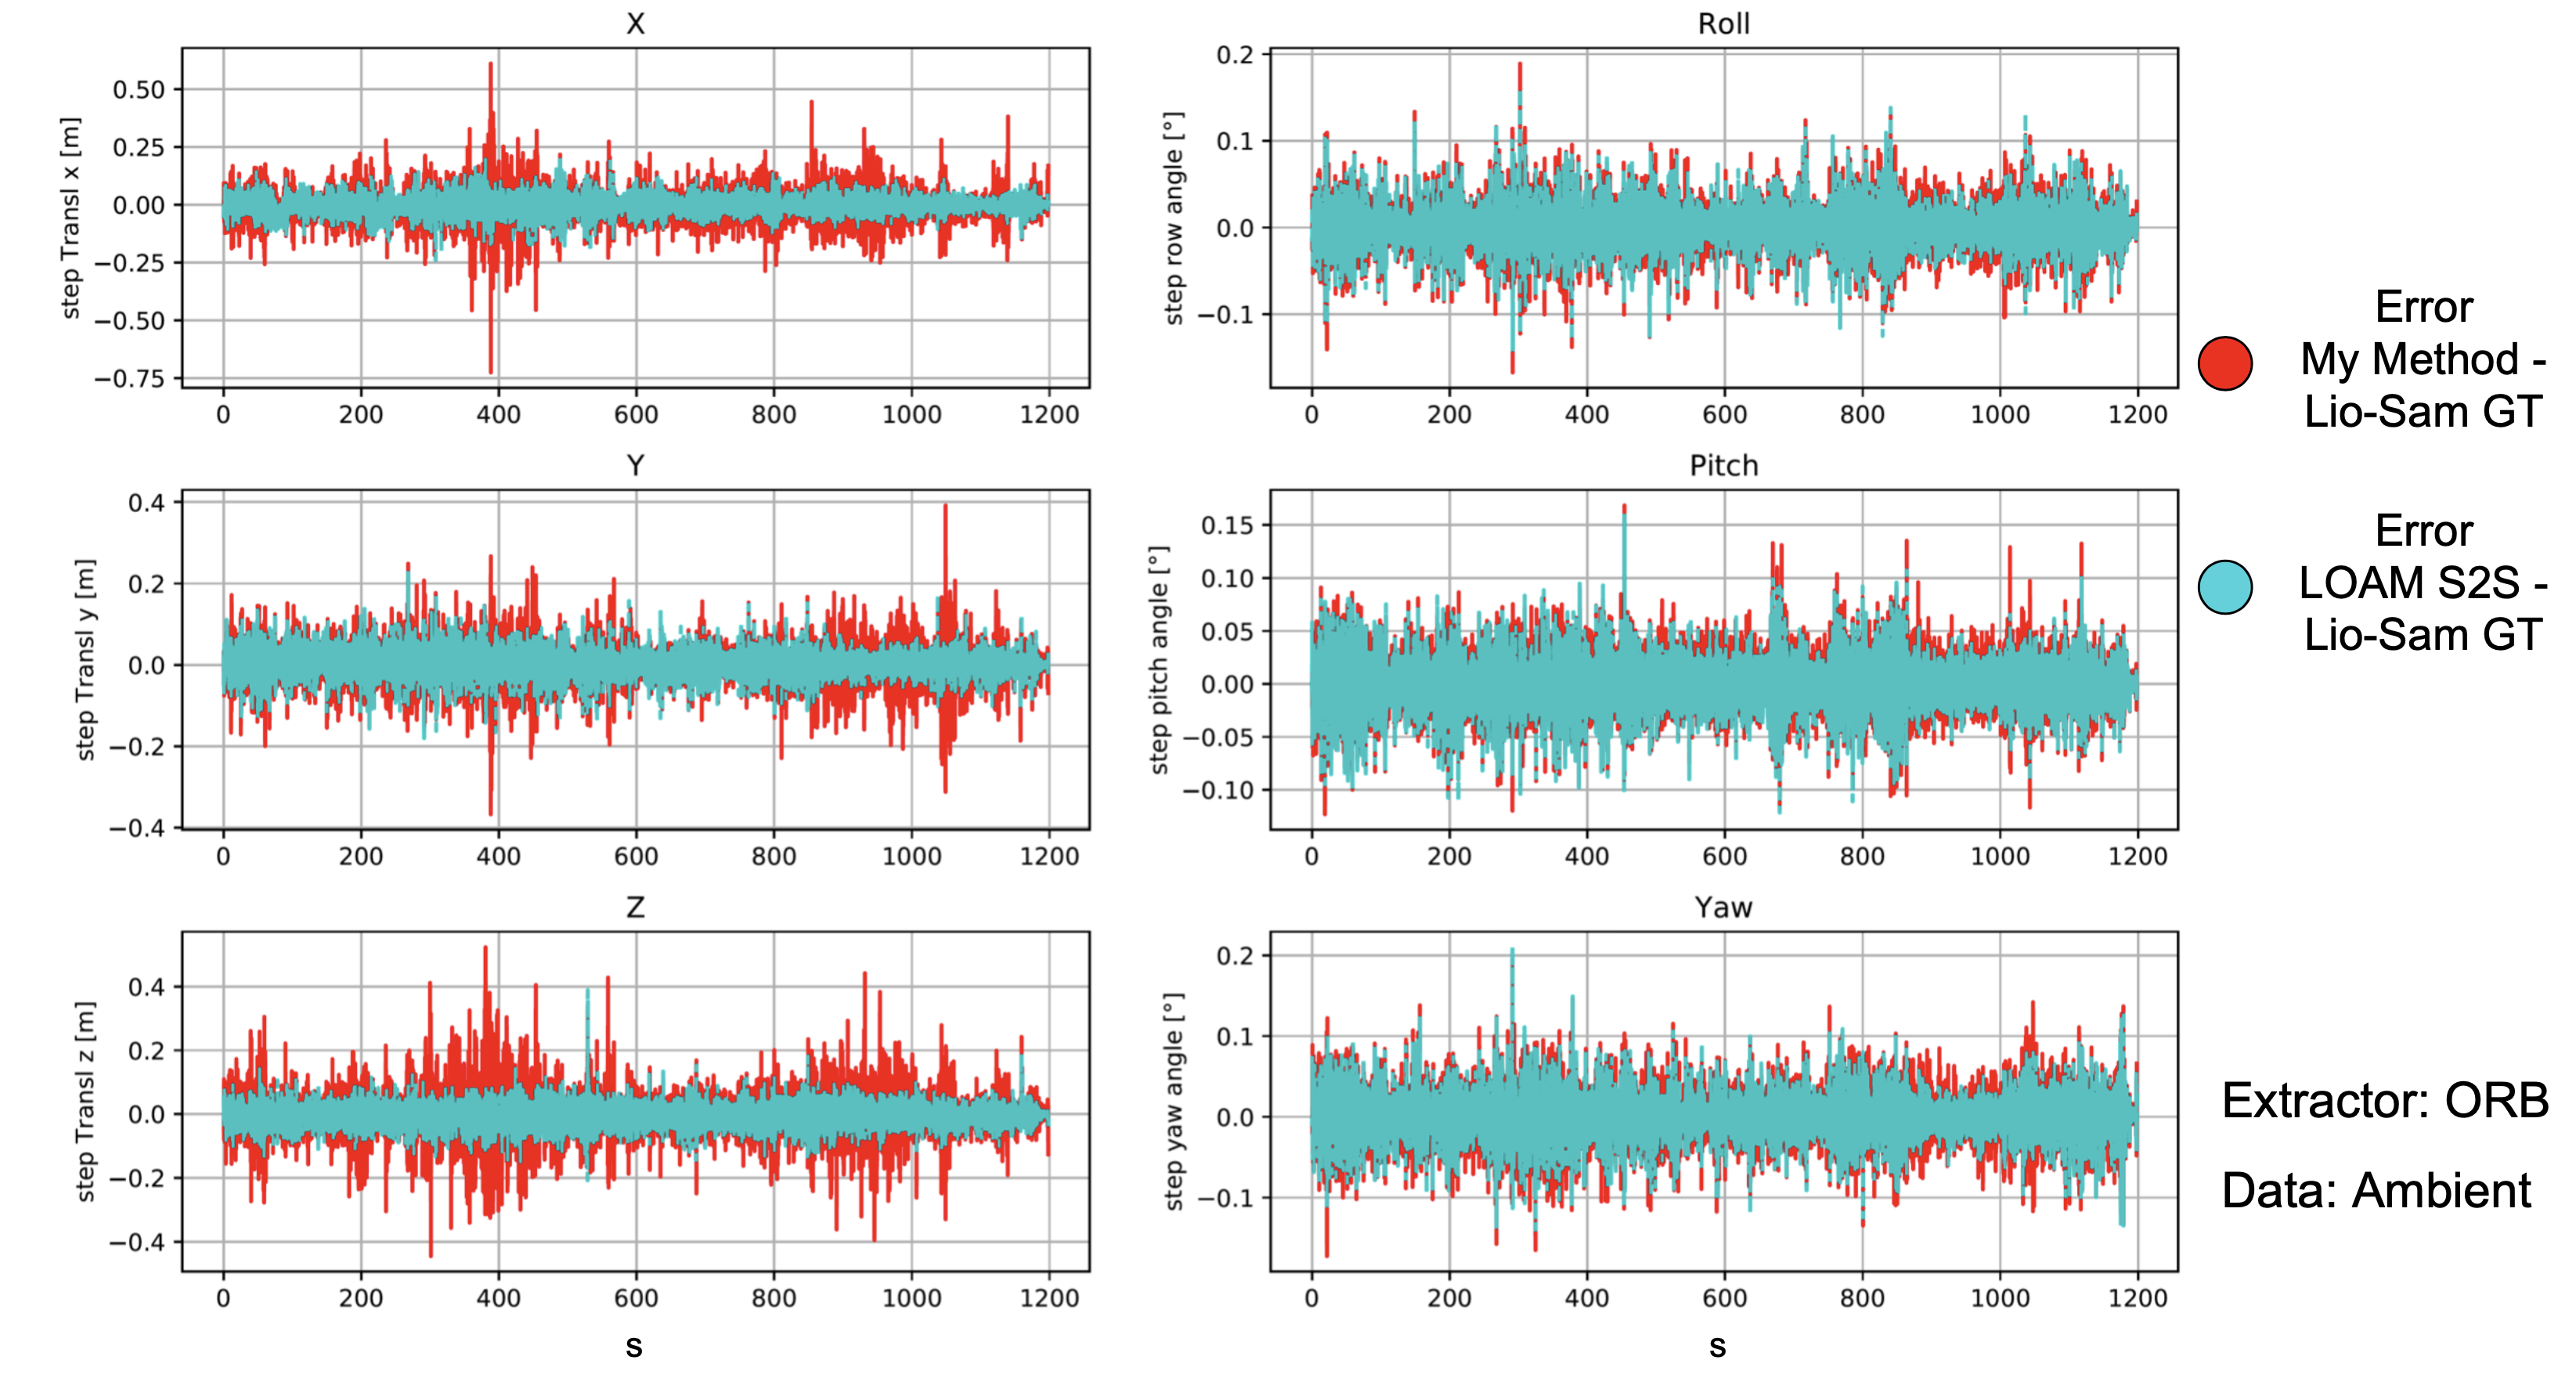
\includegraphics[scale = 0.25]{images/comparison_appendix/step_error_ambient.png}
        \caption{Step error comparison ambient}
        \label{fig:step_error_comparison_ambient}
    \end{figure}
    \clearpage
}


\section{Range Data Comparison Plots}{
    
    \begin{figure}[ht]
        \centering
        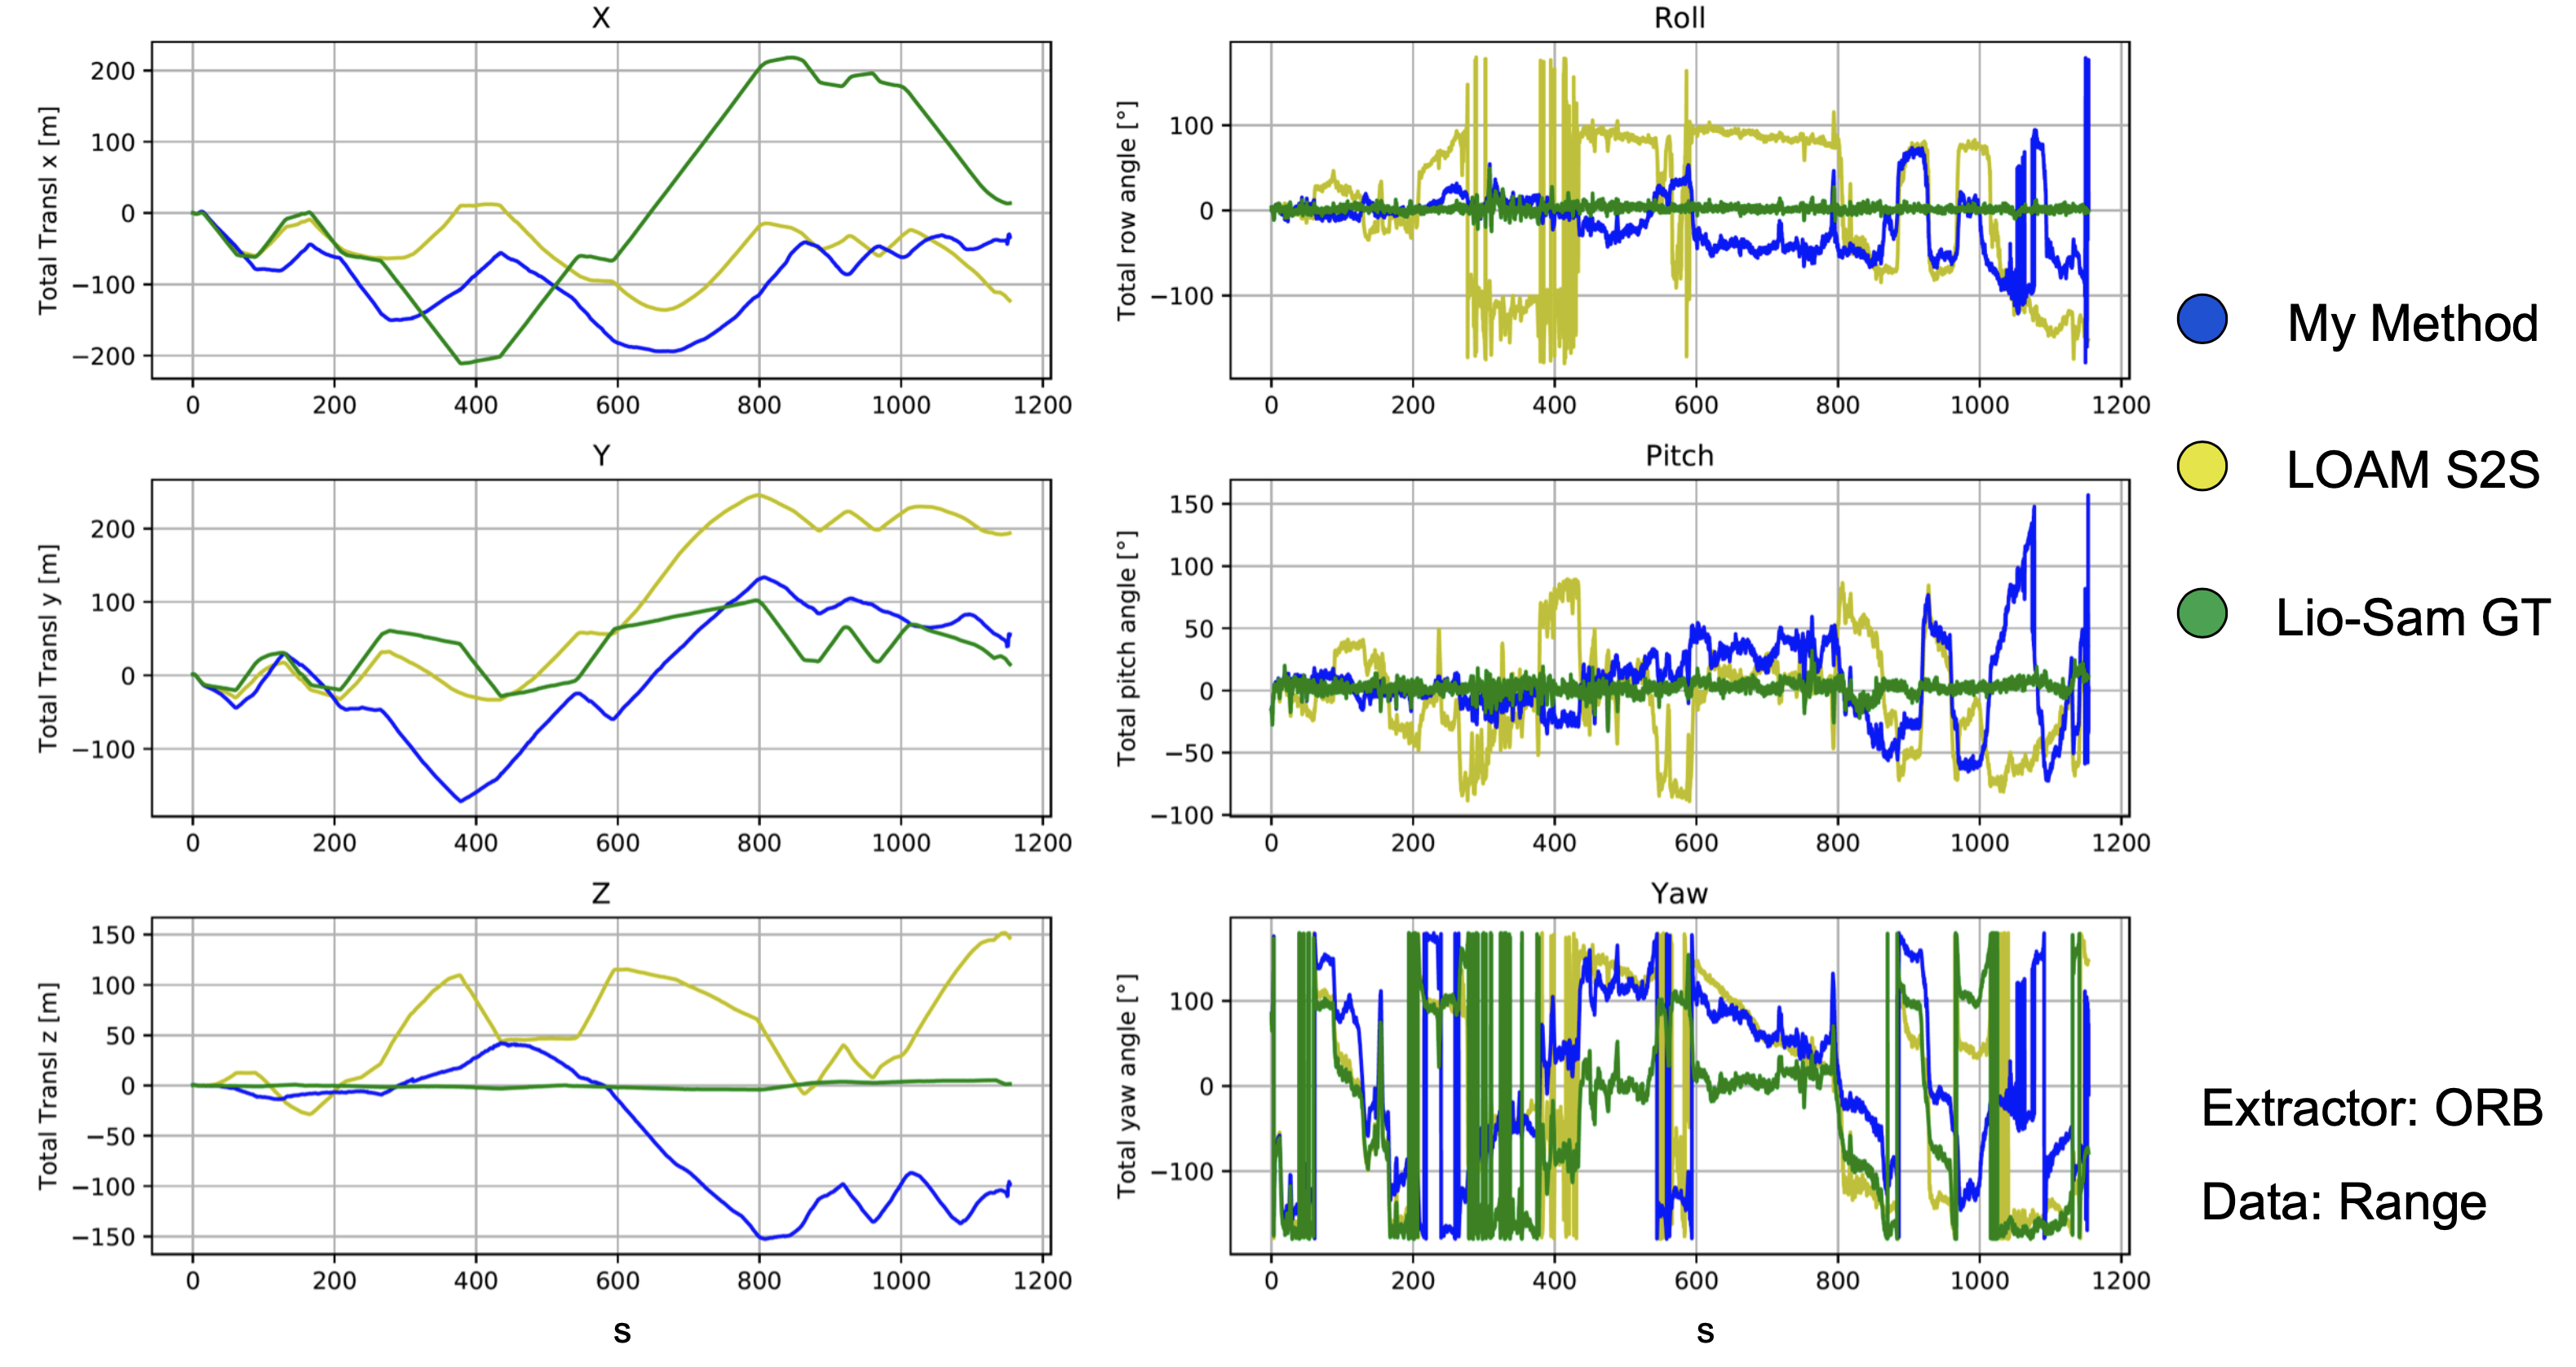
\includegraphics[scale = 0.25]{images/comparison_appendix/pose_range.png}
        \caption{Pose comparison range}
        \label{fig:pose_comparison_range}
    \end{figure}
    
    \begin{figure}[ht]
        \centering
        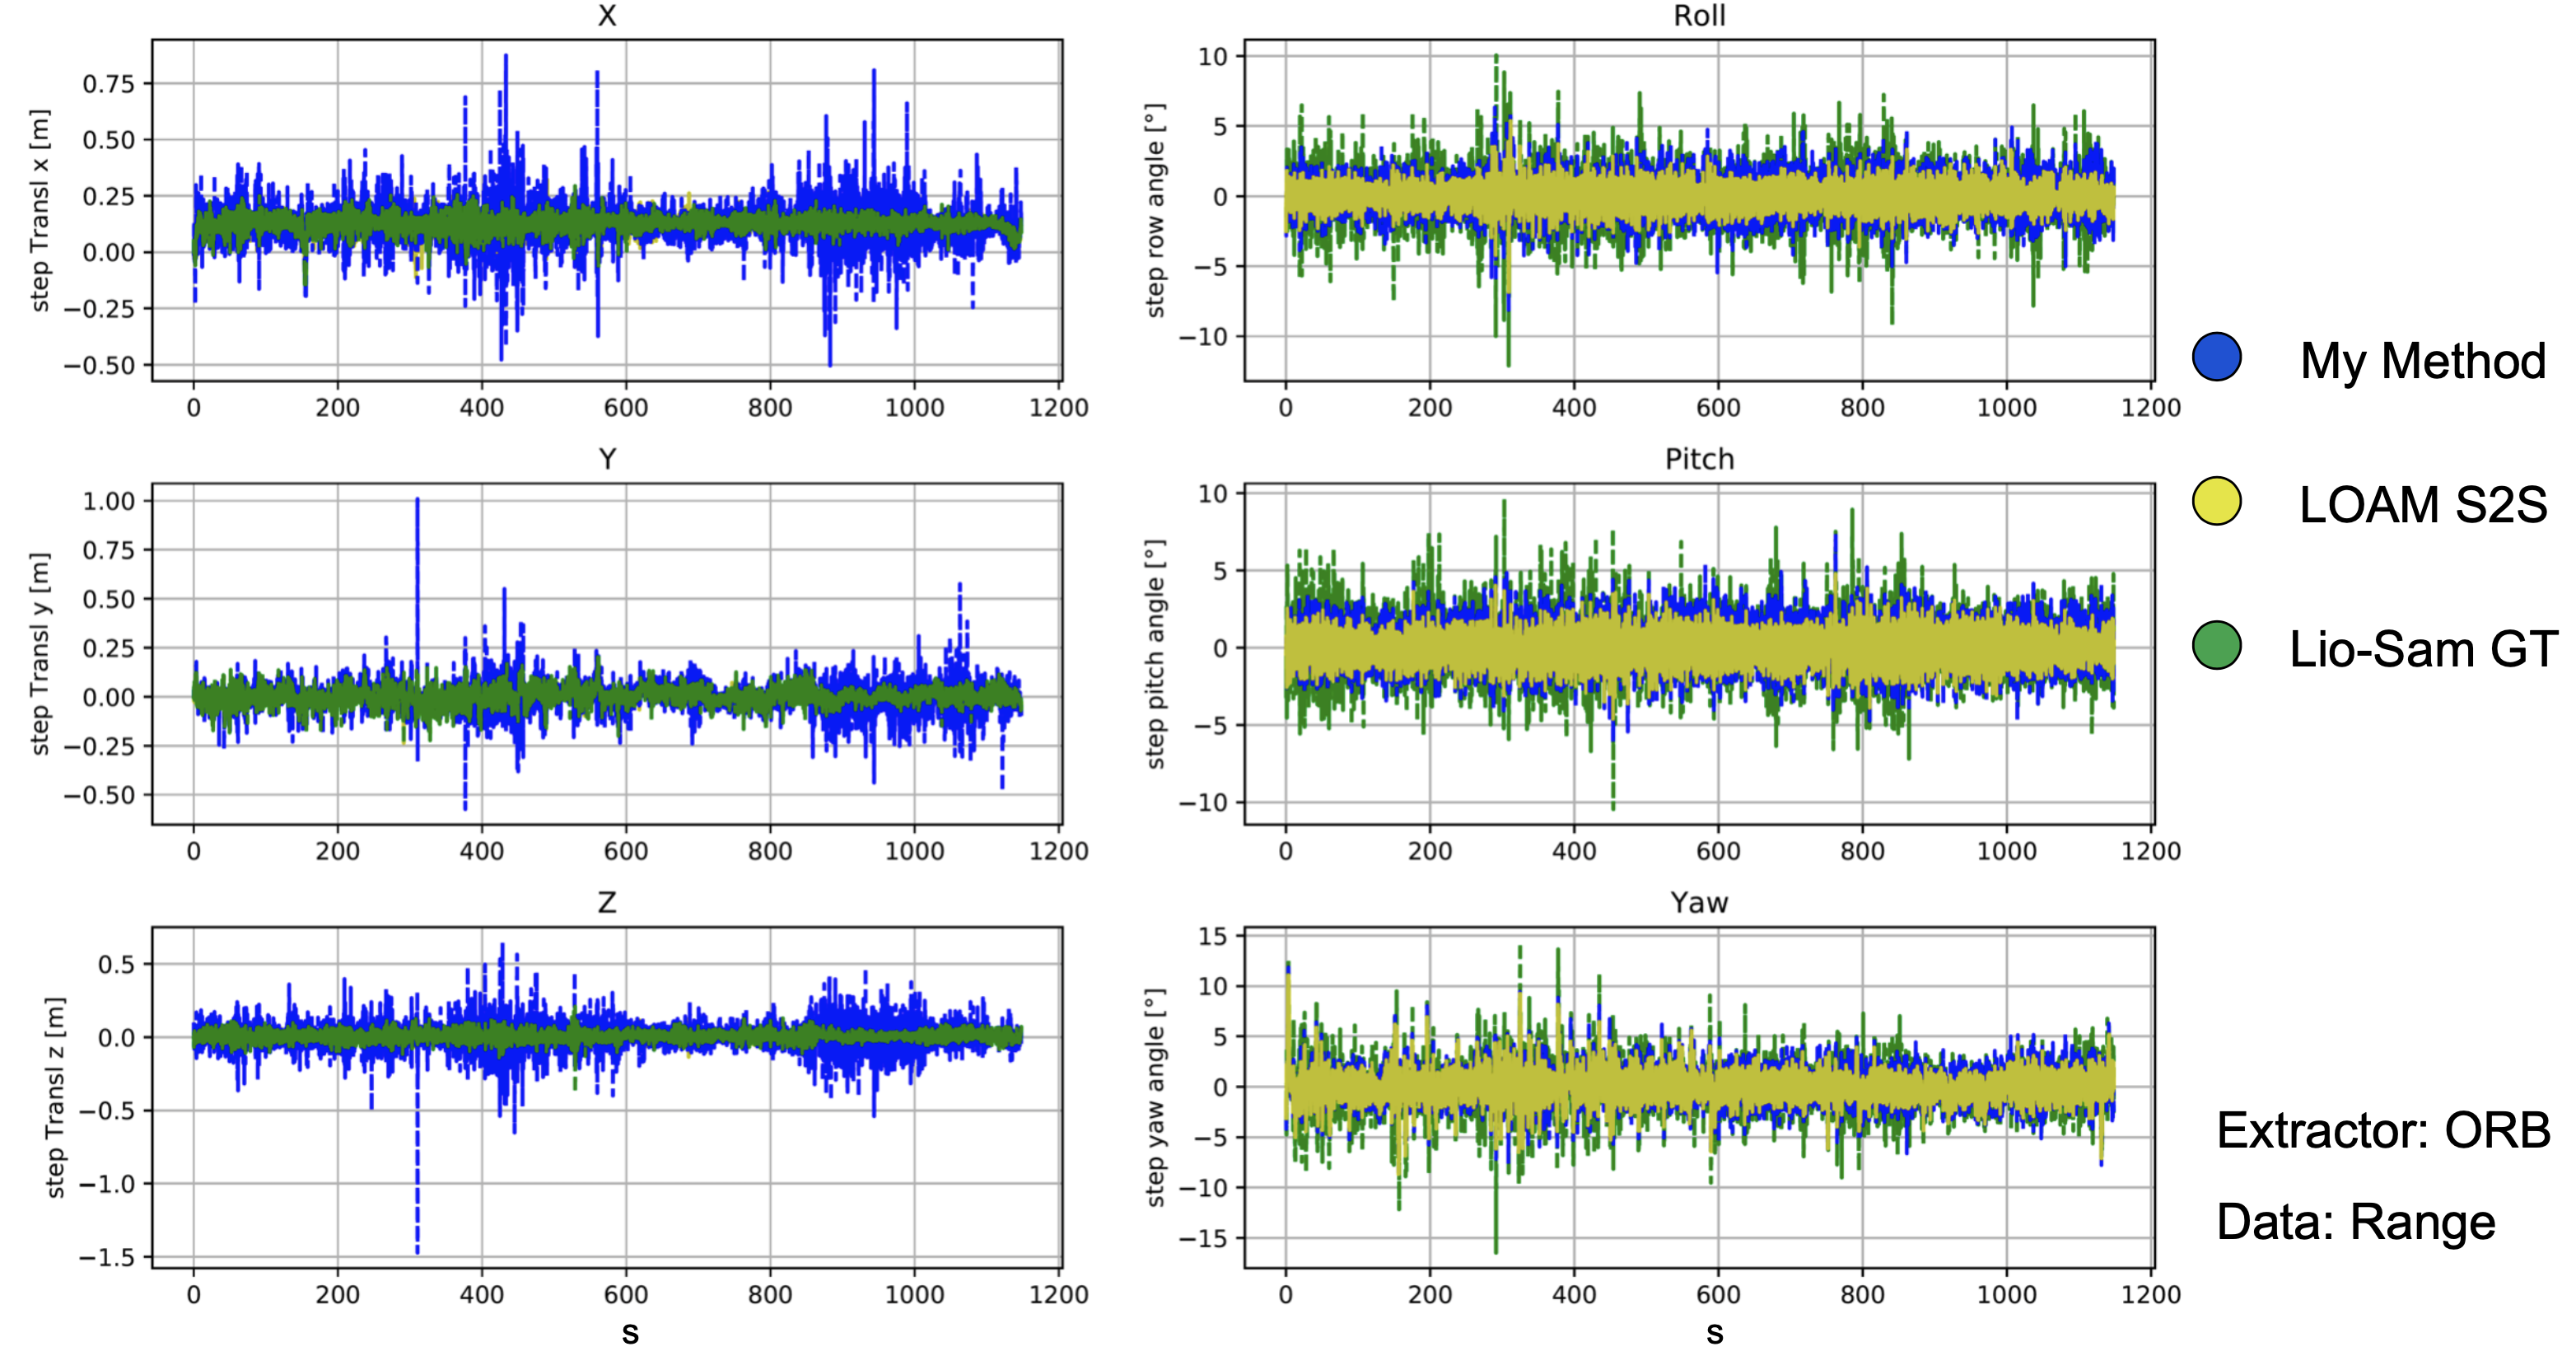
\includegraphics[scale = 0.25]{images/comparison_appendix/steps_range.png}
        \caption{Step comparison range}
        \label{fig:step_comparison_range}
    \end{figure}

    \begin{figure}[ht]
        \centering
        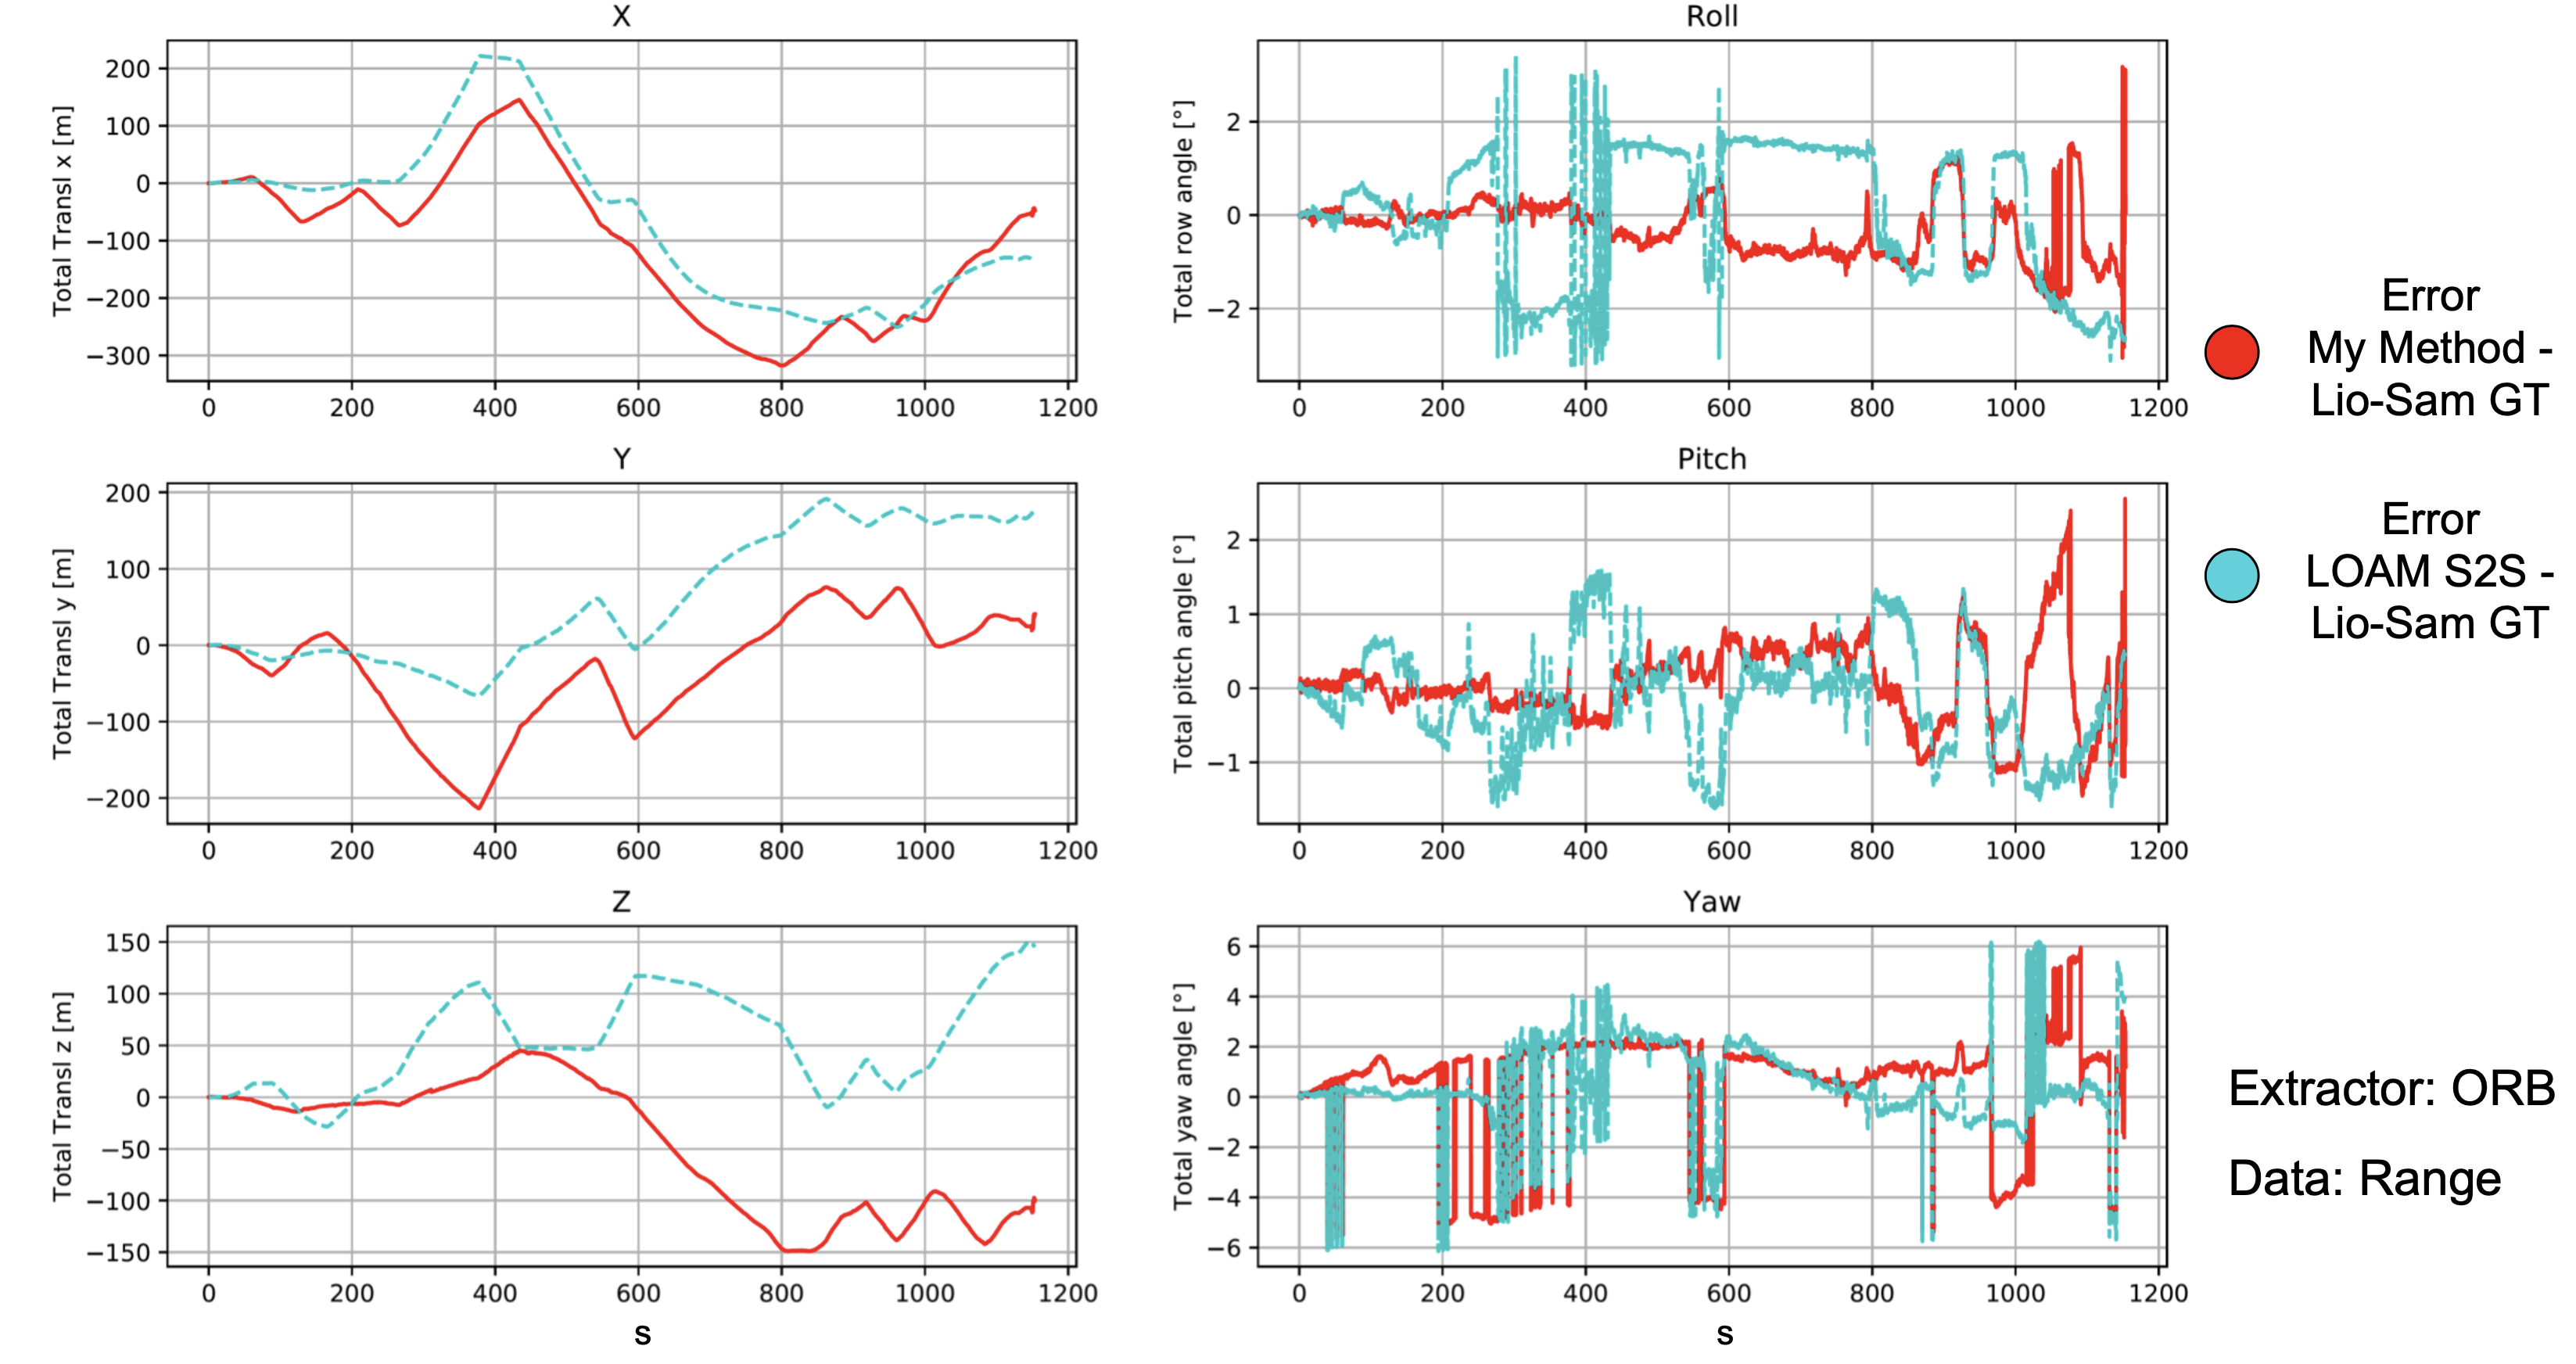
\includegraphics[scale = 0.25]{images/comparison_appendix/pose_error_range.png}
        \caption{Pose error comparison range}
        \label{fig:pose_error_comparison_range}
    \end{figure}
    
    \begin{figure}[ht]
        \centering
        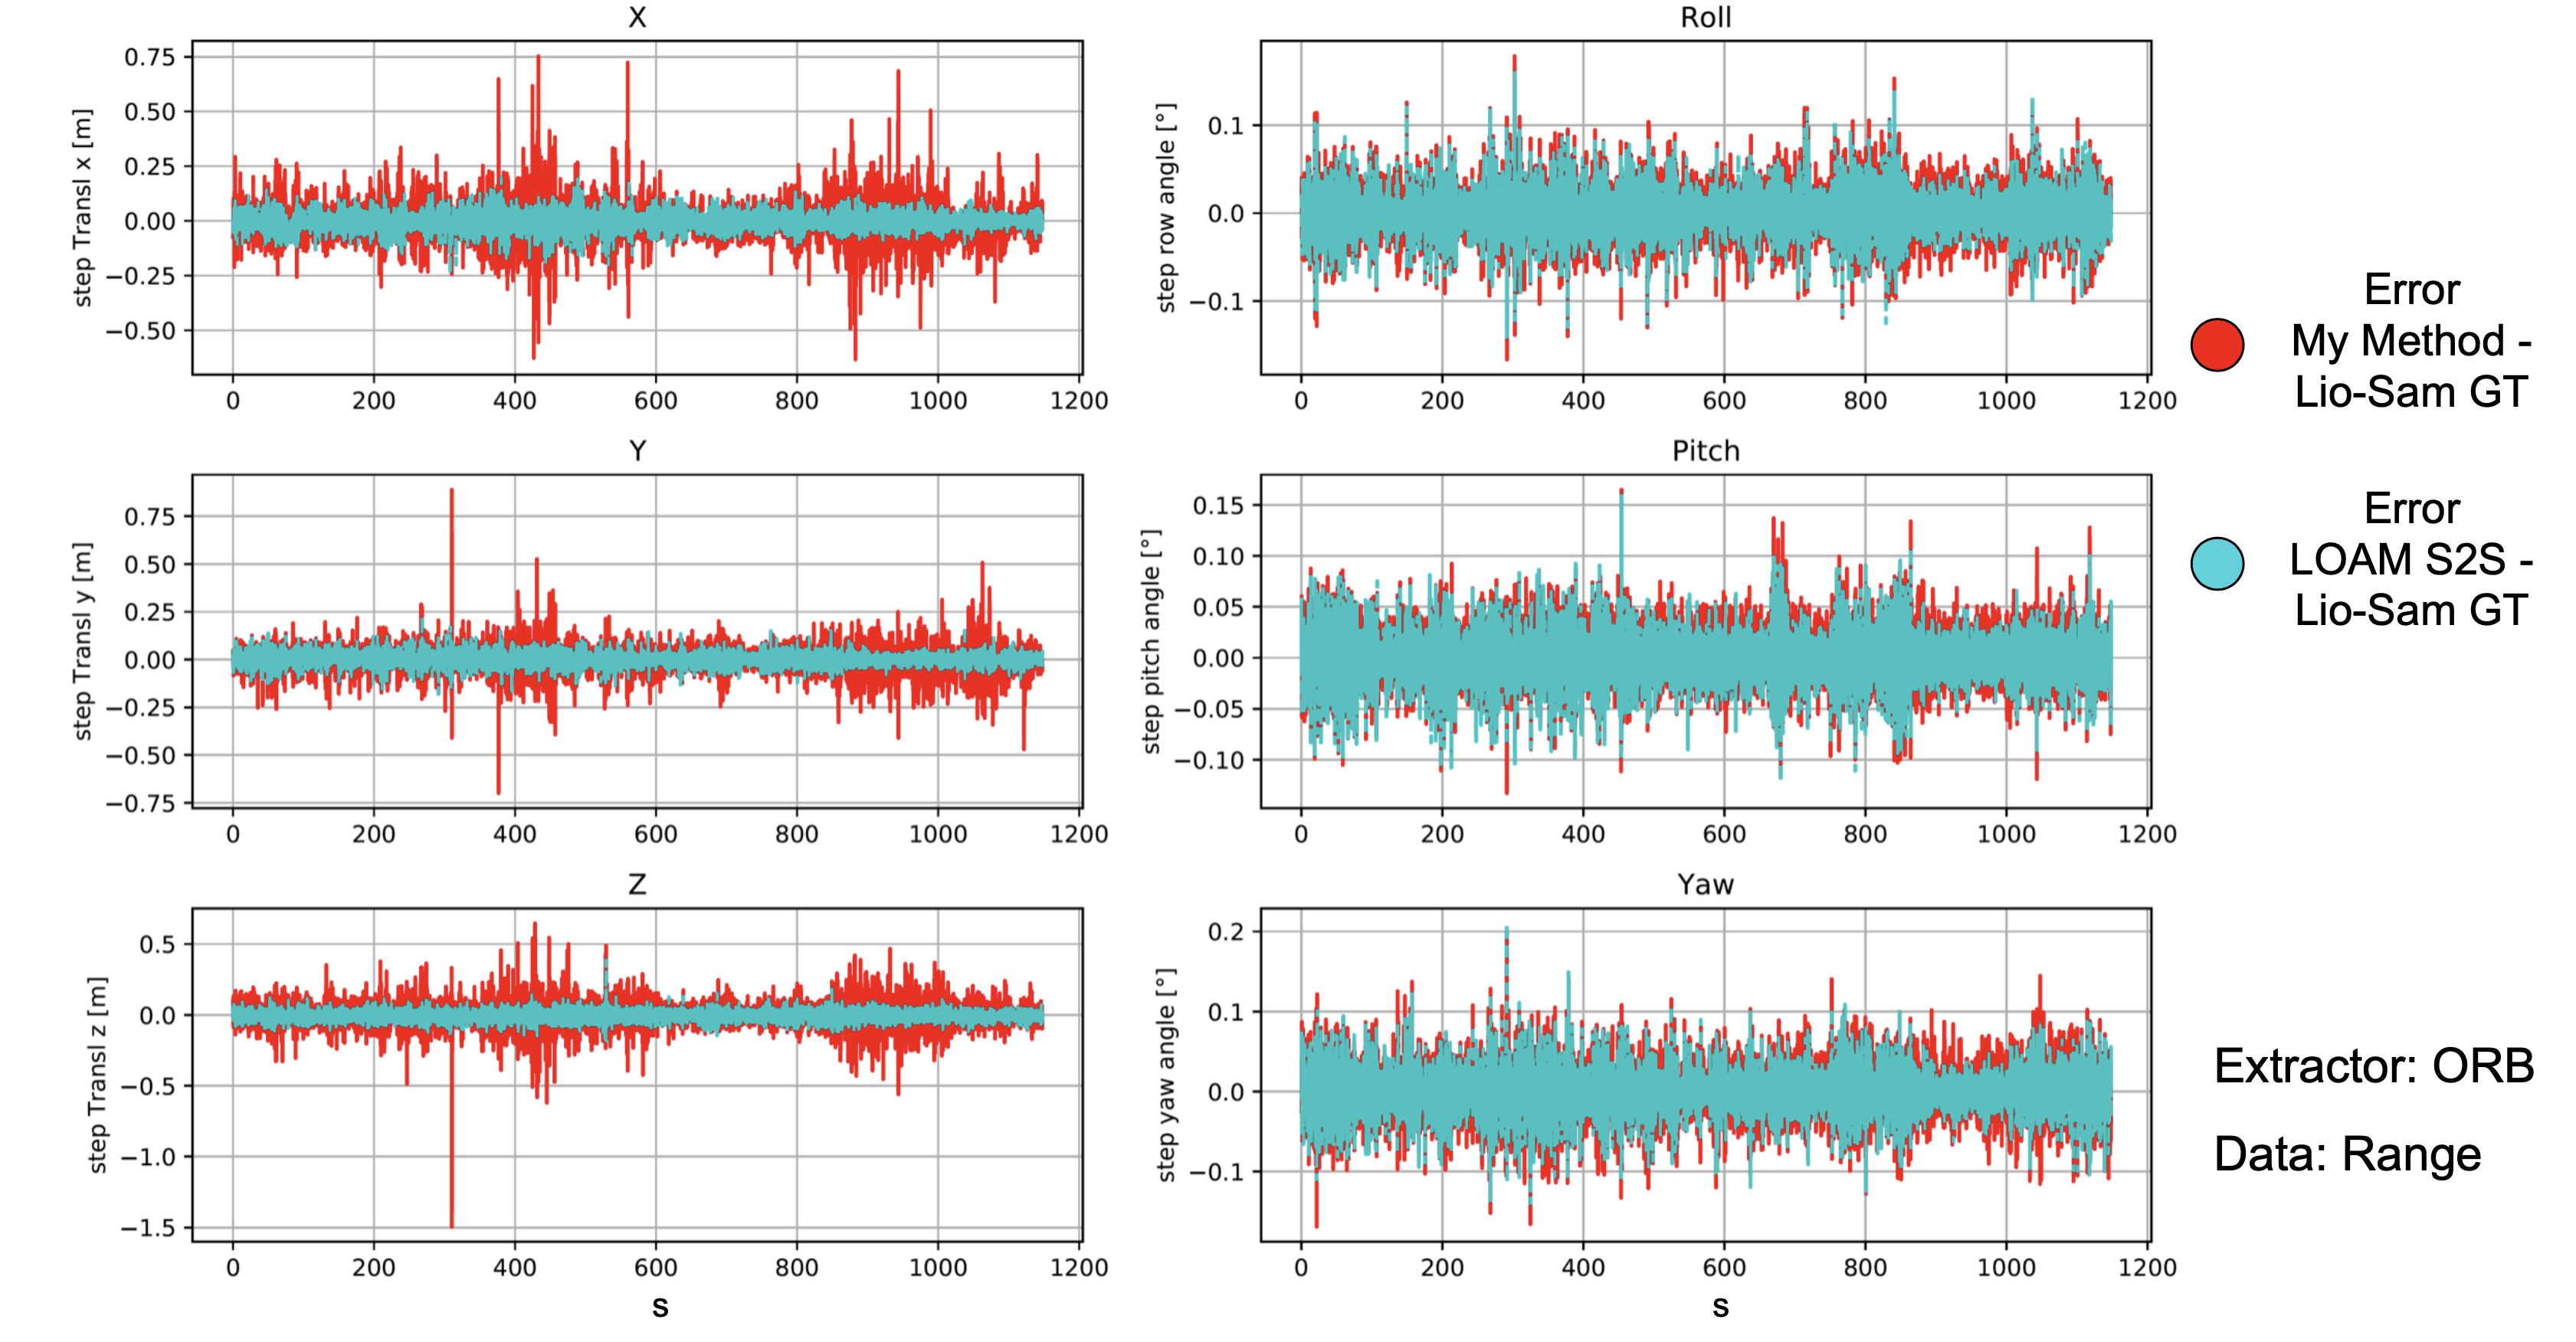
\includegraphics[scale = 0.25]{images/comparison_appendix/step_error_range.png}
        \caption{Step error comparison range}
        \label{fig:step_error_comparison_range}
    \end{figure}
    \clearpage
}

